\documentclass[english]{scrartcl}
\usepackage[osf]{mathpazo}
\usepackage[utf8]{inputenc}
\usepackage[T1]{fontenc}
\usepackage{babel}
\usepackage[usenames,dvipsnames]{color}
\usepackage{tikz}
\usepackage{gnuplot-lua-tikz}
\usepackage{amsmath,amssymb}
\usepackage{capt-of}
\usepackage{listings}
\usepackage{booktabs}
\lstset{language=xml,numbers=left,stepnumber=5,numberstyle=\ttfamily\color{Purple},basicstyle=\small\ttfamily,keywordstyle=\itshape,stringstyle=\color{Bittersweet},morekeywords={Expression,Function,Parameter,VectorField,StateVariable}}

\setcapindent{0em}
\addtokomafont{captionlabel}{\bfseries}
\addtokomafont{title}{\rmfamily}

\author{Andrei Kramer}
\title{Analysis of a large Sample}
\subject{MCMC\_CLIB}

\begin{document}
\maketitle
\begin{abstract}
  This Supplement provides some illustration for the chosen model. It
  shows, how a parameter sample is related to a model fit. This model
  has been chosen as an example for a hard problem: the model is large
  and cannot fit all of the observations simultaneously; the
  measurements are sparse, uncertain, and are provided in arbitrary
  units. Note: The reason for the missmatch will not be discussed. The
  data might have been obtained under erroneous assumptions which are
  consequently not reflected in the modeling setup or alternatively,
  the model is incorrect.
\end{abstract}
\section{Two different ways to sample the provided model}

\begin{figure}
  \hspace*{-1cm}
  % GNUPLOT: LaTeX picture with Postscript
\begingroup
  \makeatletter
  \providecommand\color[2][]{%
    \GenericError{(gnuplot) \space\space\space\@spaces}{%
      Package color not loaded in conjunction with
      terminal option `colourtext'%
    }{See the gnuplot documentation for explanation.%
    }{Either use 'blacktext' in gnuplot or load the package
      color.sty in LaTeX.}%
    \renewcommand\color[2][]{}%
  }%
  \providecommand\includegraphics[2][]{%
    \GenericError{(gnuplot) \space\space\space\@spaces}{%
      Package graphicx or graphics not loaded%
    }{See the gnuplot documentation for explanation.%
    }{The gnuplot epslatex terminal needs graphicx.sty or graphics.sty.}%
    \renewcommand\includegraphics[2][]{}%
  }%
  \providecommand\rotatebox[2]{#2}%
  \@ifundefined{ifGPcolor}{%
    \newif\ifGPcolor
    \GPcolorfalse
  }{}%
  \@ifundefined{ifGPblacktext}{%
    \newif\ifGPblacktext
    \GPblacktexttrue
  }{}%
  % define a \g@addto@macro without @ in the name:
  \let\gplgaddtomacro\g@addto@macro
  % define empty templates for all commands taking text:
  \gdef\gplbacktext{}%
  \gdef\gplfronttext{}%
  \makeatother
  \ifGPblacktext
    % no textcolor at all
    \def\colorrgb#1{}%
    \def\colorgray#1{}%
  \else
    % gray or color?
    \ifGPcolor
      \def\colorrgb#1{\color[rgb]{#1}}%
      \def\colorgray#1{\color[gray]{#1}}%
      \expandafter\def\csname LTw\endcsname{\color{white}}%
      \expandafter\def\csname LTb\endcsname{\color{black}}%
      \expandafter\def\csname LTa\endcsname{\color{black}}%
      \expandafter\def\csname LT0\endcsname{\color[rgb]{1,0,0}}%
      \expandafter\def\csname LT1\endcsname{\color[rgb]{0,1,0}}%
      \expandafter\def\csname LT2\endcsname{\color[rgb]{0,0,1}}%
      \expandafter\def\csname LT3\endcsname{\color[rgb]{1,0,1}}%
      \expandafter\def\csname LT4\endcsname{\color[rgb]{0,1,1}}%
      \expandafter\def\csname LT5\endcsname{\color[rgb]{1,1,0}}%
      \expandafter\def\csname LT6\endcsname{\color[rgb]{0,0,0}}%
      \expandafter\def\csname LT7\endcsname{\color[rgb]{1,0.3,0}}%
      \expandafter\def\csname LT8\endcsname{\color[rgb]{0.5,0.5,0.5}}%
    \else
      % gray
      \def\colorrgb#1{\color{black}}%
      \def\colorgray#1{\color[gray]{#1}}%
      \expandafter\def\csname LTw\endcsname{\color{white}}%
      \expandafter\def\csname LTb\endcsname{\color{black}}%
      \expandafter\def\csname LTa\endcsname{\color{black}}%
      \expandafter\def\csname LT0\endcsname{\color{black}}%
      \expandafter\def\csname LT1\endcsname{\color{black}}%
      \expandafter\def\csname LT2\endcsname{\color{black}}%
      \expandafter\def\csname LT3\endcsname{\color{black}}%
      \expandafter\def\csname LT4\endcsname{\color{black}}%
      \expandafter\def\csname LT5\endcsname{\color{black}}%
      \expandafter\def\csname LT6\endcsname{\color{black}}%
      \expandafter\def\csname LT7\endcsname{\color{black}}%
      \expandafter\def\csname LT8\endcsname{\color{black}}%
    \fi
  \fi
  \setlength{\unitlength}{0.0500bp}%
  \begin{picture}(9070.00,5668.00)%
    \gplgaddtomacro\gplbacktext{%
      \colorrgb{0.00,0.00,0.00}%
      \put(740,760){\makebox(0,0)[r]{\strut{}-10}}%
      \colorrgb{0.00,0.00,0.00}%
      \put(740,1644){\makebox(0,0)[r]{\strut{}-5}}%
      \colorrgb{0.00,0.00,0.00}%
      \put(740,2529){\makebox(0,0)[r]{\strut{}0}}%
      \colorrgb{0.00,0.00,0.00}%
      \put(740,3413){\makebox(0,0)[r]{\strut{}5}}%
      \colorrgb{0.00,0.00,0.00}%
      \put(740,4297){\makebox(0,0)[r]{\strut{}10}}%
      \colorrgb{0.00,0.00,0.00}%
      \put(740,5181){\makebox(0,0)[r]{\strut{}15}}%
      \colorrgb{0.00,0.00,0.00}%
      \put(2158,440){\makebox(0,0){\strut{}5}}%
      \colorrgb{0.00,0.00,0.00}%
      \put(3703,440){\makebox(0,0){\strut{}10}}%
      \colorrgb{0.00,0.00,0.00}%
      \put(5248,440){\makebox(0,0){\strut{}15}}%
      \colorrgb{0.00,0.00,0.00}%
      \put(6793,440){\makebox(0,0){\strut{}20}}%
      \colorrgb{0.00,0.00,0.00}%
      \put(8338,440){\makebox(0,0){\strut{}25}}%
      \colorrgb{0.00,0.00,0.00}%
      \put(160,3033){\rotatebox{90}{\makebox(0,0){\strut{}$\theta_i$}}}%
      \colorrgb{0.00,0.00,0.00}%
      \put(4784,140){\makebox(0,0){\strut{}$i$}}%
    }%
    \gplgaddtomacro\gplfronttext{%
      \csname LTb\endcsname%
      \put(7806,5264){\makebox(0,0)[r]{\strut{}mean}}%
    }%
    \gplbacktext
    \put(0,0){\includegraphics{sample}}%
    \gplfronttext
  \end{picture}%
\endgroup

  \caption{The Posterior Sample of size $N=1\times10^6$, as obtained
    from the \texttt{MCMC\_CLIB}; thinned out using the integrated
    autocorrelation length $\tau_{\text{int.},l}=1520(250)$ (estimated
    using the log-posterior $l$ as observable). The red line indicates
    the maximum posterior estimate, while the green errorbars indicate
    the used prior distribution (Gaussian). The colorpalette reflects
    the value of the log-posterior for each sampled point.  Here, we
    have incorporated our prior knowledge about the parameter values
    in the prior parameter density. Yet, we have chosen to let the
    prior span several orders of magnitude.\label{fig:pc-sample}}
\end{figure}

The sample was obtained in $t_{\text{s}}=267385$\,s (about
$74$\,h). Considering the auto-correlation
$\tau_{\text{int.},l}=1520(250)$, the effective sampling speed is:
\begin{equation}
  \label{eq:speed}
  v=\frac{N}{2\tau_{\text{int.},l} t_{\text{s}}}=12(2)\times 10^{-4}\,\text{s}^{-1}\,.
\end{equation}
The properties recorded during sampling are summarised in
Table~\ref{tab:sp}. The sample is plotted in
Figure~\ref{fig:pc-sample} using parallel coordinates (each sampled
parameter vector is shown component wise, as a
line). Figure~\ref{fig:osmpl} shows the output trajectories obtained
from forward simulations using the sampled parameters. There is
partial agreement between model and data (black errorbars).
\begin{figure}
  \sffamily\tiny
  \hspace*{-3cm}
  \begin{tikzpicture}
    \node (plot) {% GNUPLOT: LaTeX picture with Postscript
\begingroup
  \makeatletter
  \providecommand\color[2][]{%
    \GenericError{(gnuplot) \space\space\space\@spaces}{%
      Package color not loaded in conjunction with
      terminal option `colourtext'%
    }{See the gnuplot documentation for explanation.%
    }{Either use 'blacktext' in gnuplot or load the package
      color.sty in LaTeX.}%
    \renewcommand\color[2][]{}%
  }%
  \providecommand\includegraphics[2][]{%
    \GenericError{(gnuplot) \space\space\space\@spaces}{%
      Package graphicx or graphics not loaded%
    }{See the gnuplot documentation for explanation.%
    }{The gnuplot epslatex terminal needs graphicx.sty or graphics.sty.}%
    \renewcommand\includegraphics[2][]{}%
  }%
  \providecommand\rotatebox[2]{#2}%
  \@ifundefined{ifGPcolor}{%
    \newif\ifGPcolor
    \GPcolorfalse
  }{}%
  \@ifundefined{ifGPblacktext}{%
    \newif\ifGPblacktext
    \GPblacktexttrue
  }{}%
  % define a \g@addto@macro without @ in the name:
  \let\gplgaddtomacro\g@addto@macro
  % define empty templates for all commands taking text:
  \gdef\gplbacktext{}%
  \gdef\gplfronttext{}%
  \makeatother
  \ifGPblacktext
    % no textcolor at all
    \def\colorrgb#1{}%
    \def\colorgray#1{}%
  \else
    % gray or color?
    \ifGPcolor
      \def\colorrgb#1{\color[rgb]{#1}}%
      \def\colorgray#1{\color[gray]{#1}}%
      \expandafter\def\csname LTw\endcsname{\color{white}}%
      \expandafter\def\csname LTb\endcsname{\color{black}}%
      \expandafter\def\csname LTa\endcsname{\color{black}}%
      \expandafter\def\csname LT0\endcsname{\color[rgb]{1,0,0}}%
      \expandafter\def\csname LT1\endcsname{\color[rgb]{0,1,0}}%
      \expandafter\def\csname LT2\endcsname{\color[rgb]{0,0,1}}%
      \expandafter\def\csname LT3\endcsname{\color[rgb]{1,0,1}}%
      \expandafter\def\csname LT4\endcsname{\color[rgb]{0,1,1}}%
      \expandafter\def\csname LT5\endcsname{\color[rgb]{1,1,0}}%
      \expandafter\def\csname LT6\endcsname{\color[rgb]{0,0,0}}%
      \expandafter\def\csname LT7\endcsname{\color[rgb]{1,0.3,0}}%
      \expandafter\def\csname LT8\endcsname{\color[rgb]{0.5,0.5,0.5}}%
    \else
      % gray
      \def\colorrgb#1{\color{black}}%
      \def\colorgray#1{\color[gray]{#1}}%
      \expandafter\def\csname LTw\endcsname{\color{white}}%
      \expandafter\def\csname LTb\endcsname{\color{black}}%
      \expandafter\def\csname LTa\endcsname{\color{black}}%
      \expandafter\def\csname LT0\endcsname{\color{black}}%
      \expandafter\def\csname LT1\endcsname{\color{black}}%
      \expandafter\def\csname LT2\endcsname{\color{black}}%
      \expandafter\def\csname LT3\endcsname{\color{black}}%
      \expandafter\def\csname LT4\endcsname{\color{black}}%
      \expandafter\def\csname LT5\endcsname{\color{black}}%
      \expandafter\def\csname LT6\endcsname{\color{black}}%
      \expandafter\def\csname LT7\endcsname{\color{black}}%
      \expandafter\def\csname LT8\endcsname{\color{black}}%
    \fi
  \fi
  \setlength{\unitlength}{0.0500bp}%
  \begin{picture}(11520.00,8640.00)%
    \gplgaddtomacro\gplbacktext{%
      \colorrgb{0.00,0.00,0.00}%
      \put(1377,6629){\makebox(0,0)[r]{\strut{}0}}%
      \colorrgb{0.00,0.00,0.00}%
      \put(1377,6856){\makebox(0,0)[r]{\strut{}1}}%
      \colorrgb{0.00,0.00,0.00}%
      \put(1377,7084){\makebox(0,0)[r]{\strut{}2}}%
      \colorrgb{0.00,0.00,0.00}%
      \put(1377,7311){\makebox(0,0)[r]{\strut{}3}}%
      \colorrgb{0.00,0.00,0.00}%
      \put(1377,7538){\makebox(0,0)[r]{\strut{}4}}%
      \colorrgb{0.00,0.00,0.00}%
      \put(1377,7766){\makebox(0,0)[r]{\strut{}5}}%
      \colorrgb{0.00,0.00,0.00}%
      \put(1377,7993){\makebox(0,0)[r]{\strut{}6}}%
      \colorrgb{0.00,0.00,0.00}%
      \put(2087,6429){\makebox(0,0){\strut{}.1}}%
      \colorrgb{0.00,0.00,0.00}%
      \put(2145,6429){\makebox(0,0){\strut{}8}}%
      \colorrgb{0.00,0.00,0.00}%
      \put(2264,6429){\makebox(0,0){\strut{}24}}%
      \colorrgb{0.00,0.00,0.00}%
      \put(2443,6429){\makebox(0,0){\strut{}48}}%
      \colorrgb{0.00,0.00,0.00}%
      \put(2621,6429){\makebox(0,0){\strut{}72}}%
    }%
    \gplgaddtomacro\gplfronttext{%
    }%
    \gplgaddtomacro\gplbacktext{%
      \colorrgb{0.00,0.00,0.00}%
      \put(2927,6629){\makebox(0,0)[r]{\strut{}0}}%
      \colorrgb{0.00,0.00,0.00}%
      \put(2927,6804){\makebox(0,0)[r]{\strut{}0.2}}%
      \colorrgb{0.00,0.00,0.00}%
      \put(2927,6979){\makebox(0,0)[r]{\strut{}0.4}}%
      \colorrgb{0.00,0.00,0.00}%
      \put(2927,7154){\makebox(0,0)[r]{\strut{}0.6}}%
      \colorrgb{0.00,0.00,0.00}%
      \put(2927,7328){\makebox(0,0)[r]{\strut{}0.8}}%
      \colorrgb{0.00,0.00,0.00}%
      \put(2927,7503){\makebox(0,0)[r]{\strut{}1}}%
      \colorrgb{0.00,0.00,0.00}%
      \put(2927,7678){\makebox(0,0)[r]{\strut{}1.2}}%
      \colorrgb{0.00,0.00,0.00}%
      \put(2927,7853){\makebox(0,0)[r]{\strut{}1.4}}%
      \colorrgb{0.00,0.00,0.00}%
      \put(3637,6429){\makebox(0,0){\strut{}.1}}%
      \colorrgb{0.00,0.00,0.00}%
      \put(3695,6429){\makebox(0,0){\strut{}8}}%
      \colorrgb{0.00,0.00,0.00}%
      \put(3814,6429){\makebox(0,0){\strut{}24}}%
      \colorrgb{0.00,0.00,0.00}%
      \put(3993,6429){\makebox(0,0){\strut{}48}}%
      \colorrgb{0.00,0.00,0.00}%
      \put(4171,6429){\makebox(0,0){\strut{}72}}%
    }%
    \gplgaddtomacro\gplfronttext{%
    }%
    \gplgaddtomacro\gplbacktext{%
      \colorrgb{0.00,0.00,0.00}%
      \put(4477,6629){\makebox(0,0)[r]{\strut{}0}}%
      \colorrgb{0.00,0.00,0.00}%
      \put(4477,6868){\makebox(0,0)[r]{\strut{}0.2}}%
      \colorrgb{0.00,0.00,0.00}%
      \put(4477,7107){\makebox(0,0)[r]{\strut{}0.4}}%
      \colorrgb{0.00,0.00,0.00}%
      \put(4477,7346){\makebox(0,0)[r]{\strut{}0.6}}%
      \colorrgb{0.00,0.00,0.00}%
      \put(4477,7585){\makebox(0,0)[r]{\strut{}0.8}}%
      \colorrgb{0.00,0.00,0.00}%
      \put(4477,7824){\makebox(0,0)[r]{\strut{}1}}%
      \colorrgb{0.00,0.00,0.00}%
      \put(5187,6429){\makebox(0,0){\strut{}.1}}%
      \colorrgb{0.00,0.00,0.00}%
      \put(5245,6429){\makebox(0,0){\strut{}8}}%
      \colorrgb{0.00,0.00,0.00}%
      \put(5364,6429){\makebox(0,0){\strut{}24}}%
      \colorrgb{0.00,0.00,0.00}%
      \put(5543,6429){\makebox(0,0){\strut{}48}}%
      \colorrgb{0.00,0.00,0.00}%
      \put(5721,6429){\makebox(0,0){\strut{}72}}%
    }%
    \gplgaddtomacro\gplfronttext{%
    }%
    \gplgaddtomacro\gplbacktext{%
      \colorrgb{0.00,0.00,0.00}%
      \put(6027,6629){\makebox(0,0)[r]{\strut{}0}}%
      \colorrgb{0.00,0.00,0.00}%
      \put(6027,6872){\makebox(0,0)[r]{\strut{}0.2}}%
      \colorrgb{0.00,0.00,0.00}%
      \put(6027,7114){\makebox(0,0)[r]{\strut{}0.4}}%
      \colorrgb{0.00,0.00,0.00}%
      \put(6027,7357){\makebox(0,0)[r]{\strut{}0.6}}%
      \colorrgb{0.00,0.00,0.00}%
      \put(6027,7599){\makebox(0,0)[r]{\strut{}0.8}}%
      \colorrgb{0.00,0.00,0.00}%
      \put(6027,7842){\makebox(0,0)[r]{\strut{}1}}%
      \colorrgb{0.00,0.00,0.00}%
      \put(6736,6429){\makebox(0,0){\strut{}.1}}%
      \colorrgb{0.00,0.00,0.00}%
      \put(6795,6429){\makebox(0,0){\strut{}8}}%
      \colorrgb{0.00,0.00,0.00}%
      \put(6914,6429){\makebox(0,0){\strut{}24}}%
      \colorrgb{0.00,0.00,0.00}%
      \put(7092,6429){\makebox(0,0){\strut{}48}}%
      \colorrgb{0.00,0.00,0.00}%
      \put(7271,6429){\makebox(0,0){\strut{}72}}%
    }%
    \gplgaddtomacro\gplfronttext{%
    }%
    \gplgaddtomacro\gplbacktext{%
      \colorrgb{0.00,0.00,0.00}%
      \put(7577,6629){\makebox(0,0)[r]{\strut{}0}}%
      \colorrgb{0.00,0.00,0.00}%
      \put(7577,6805){\makebox(0,0)[r]{\strut{}0.2}}%
      \colorrgb{0.00,0.00,0.00}%
      \put(7577,6982){\makebox(0,0)[r]{\strut{}0.4}}%
      \colorrgb{0.00,0.00,0.00}%
      \put(7577,7158){\makebox(0,0)[r]{\strut{}0.6}}%
      \colorrgb{0.00,0.00,0.00}%
      \put(7577,7335){\makebox(0,0)[r]{\strut{}0.8}}%
      \colorrgb{0.00,0.00,0.00}%
      \put(7577,7511){\makebox(0,0)[r]{\strut{}1}}%
      \colorrgb{0.00,0.00,0.00}%
      \put(7577,7688){\makebox(0,0)[r]{\strut{}1.2}}%
      \colorrgb{0.00,0.00,0.00}%
      \put(7577,7864){\makebox(0,0)[r]{\strut{}1.4}}%
      \colorrgb{0.00,0.00,0.00}%
      \put(8286,6429){\makebox(0,0){\strut{}.1}}%
      \colorrgb{0.00,0.00,0.00}%
      \put(8345,6429){\makebox(0,0){\strut{}8}}%
      \colorrgb{0.00,0.00,0.00}%
      \put(8464,6429){\makebox(0,0){\strut{}24}}%
      \colorrgb{0.00,0.00,0.00}%
      \put(8642,6429){\makebox(0,0){\strut{}48}}%
      \colorrgb{0.00,0.00,0.00}%
      \put(8821,6429){\makebox(0,0){\strut{}72}}%
    }%
    \gplgaddtomacro\gplfronttext{%
    }%
    \gplgaddtomacro\gplbacktext{%
      \colorrgb{0.00,0.00,0.00}%
      \put(9127,6629){\makebox(0,0)[r]{\strut{}0}}%
      \colorrgb{0.00,0.00,0.00}%
      \put(9127,6877){\makebox(0,0)[r]{\strut{}0.2}}%
      \colorrgb{0.00,0.00,0.00}%
      \put(9127,7124){\makebox(0,0)[r]{\strut{}0.4}}%
      \colorrgb{0.00,0.00,0.00}%
      \put(9127,7372){\makebox(0,0)[r]{\strut{}0.6}}%
      \colorrgb{0.00,0.00,0.00}%
      \put(9127,7620){\makebox(0,0)[r]{\strut{}0.8}}%
      \colorrgb{0.00,0.00,0.00}%
      \put(9127,7867){\makebox(0,0)[r]{\strut{}1}}%
      \colorrgb{0.00,0.00,0.00}%
      \put(9836,6429){\makebox(0,0){\strut{}.1}}%
      \colorrgb{0.00,0.00,0.00}%
      \put(9895,6429){\makebox(0,0){\strut{}8}}%
      \colorrgb{0.00,0.00,0.00}%
      \put(10014,6429){\makebox(0,0){\strut{}24}}%
      \colorrgb{0.00,0.00,0.00}%
      \put(10192,6429){\makebox(0,0){\strut{}48}}%
      \colorrgb{0.00,0.00,0.00}%
      \put(10371,6429){\makebox(0,0){\strut{}72}}%
    }%
    \gplgaddtomacro\gplfronttext{%
    }%
    \gplgaddtomacro\gplbacktext{%
      \colorrgb{0.00,0.00,0.00}%
      \put(1377,4736){\makebox(0,0)[r]{\strut{}0}}%
      \colorrgb{0.00,0.00,0.00}%
      \put(1377,5051){\makebox(0,0)[r]{\strut{}0.5}}%
      \colorrgb{0.00,0.00,0.00}%
      \put(1377,5366){\makebox(0,0)[r]{\strut{}1}}%
      \colorrgb{0.00,0.00,0.00}%
      \put(1377,5681){\makebox(0,0)[r]{\strut{}1.5}}%
      \colorrgb{0.00,0.00,0.00}%
      \put(1377,5996){\makebox(0,0)[r]{\strut{}2}}%
      \colorrgb{0.00,0.00,0.00}%
      \put(2087,4536){\makebox(0,0){\strut{}.1}}%
      \colorrgb{0.00,0.00,0.00}%
      \put(2145,4536){\makebox(0,0){\strut{}8}}%
      \colorrgb{0.00,0.00,0.00}%
      \put(2264,4536){\makebox(0,0){\strut{}24}}%
      \colorrgb{0.00,0.00,0.00}%
      \put(2443,4536){\makebox(0,0){\strut{}48}}%
      \colorrgb{0.00,0.00,0.00}%
      \put(2621,4536){\makebox(0,0){\strut{}72}}%
    }%
    \gplgaddtomacro\gplfronttext{%
    }%
    \gplgaddtomacro\gplbacktext{%
      \colorrgb{0.00,0.00,0.00}%
      \put(2927,4736){\makebox(0,0)[r]{\strut{}0}}%
      \colorrgb{0.00,0.00,0.00}%
      \put(2927,5031){\makebox(0,0)[r]{\strut{}0.5}}%
      \colorrgb{0.00,0.00,0.00}%
      \put(2927,5325){\makebox(0,0)[r]{\strut{}1}}%
      \colorrgb{0.00,0.00,0.00}%
      \put(2927,5620){\makebox(0,0)[r]{\strut{}1.5}}%
      \colorrgb{0.00,0.00,0.00}%
      \put(2927,5914){\makebox(0,0)[r]{\strut{}2}}%
      \colorrgb{0.00,0.00,0.00}%
      \put(3637,4536){\makebox(0,0){\strut{}.1}}%
      \colorrgb{0.00,0.00,0.00}%
      \put(3695,4536){\makebox(0,0){\strut{}8}}%
      \colorrgb{0.00,0.00,0.00}%
      \put(3814,4536){\makebox(0,0){\strut{}24}}%
      \colorrgb{0.00,0.00,0.00}%
      \put(3993,4536){\makebox(0,0){\strut{}48}}%
      \colorrgb{0.00,0.00,0.00}%
      \put(4171,4536){\makebox(0,0){\strut{}72}}%
    }%
    \gplgaddtomacro\gplfronttext{%
    }%
    \gplgaddtomacro\gplbacktext{%
      \colorrgb{0.00,0.00,0.00}%
      \put(4477,4736){\makebox(0,0)[r]{\strut{}0}}%
      \colorrgb{0.00,0.00,0.00}%
      \put(4477,4974){\makebox(0,0)[r]{\strut{}0.2}}%
      \colorrgb{0.00,0.00,0.00}%
      \put(4477,5212){\makebox(0,0)[r]{\strut{}0.4}}%
      \colorrgb{0.00,0.00,0.00}%
      \put(4477,5450){\makebox(0,0)[r]{\strut{}0.6}}%
      \colorrgb{0.00,0.00,0.00}%
      \put(4477,5688){\makebox(0,0)[r]{\strut{}0.8}}%
      \colorrgb{0.00,0.00,0.00}%
      \put(4477,5927){\makebox(0,0)[r]{\strut{}1}}%
      \colorrgb{0.00,0.00,0.00}%
      \put(5187,4536){\makebox(0,0){\strut{}.1}}%
      \colorrgb{0.00,0.00,0.00}%
      \put(5245,4536){\makebox(0,0){\strut{}8}}%
      \colorrgb{0.00,0.00,0.00}%
      \put(5364,4536){\makebox(0,0){\strut{}24}}%
      \colorrgb{0.00,0.00,0.00}%
      \put(5543,4536){\makebox(0,0){\strut{}48}}%
      \colorrgb{0.00,0.00,0.00}%
      \put(5721,4536){\makebox(0,0){\strut{}72}}%
    }%
    \gplgaddtomacro\gplfronttext{%
    }%
    \gplgaddtomacro\gplbacktext{%
      \colorrgb{0.00,0.00,0.00}%
      \put(6027,4736){\makebox(0,0)[r]{\strut{}0}}%
      \colorrgb{0.00,0.00,0.00}%
      \put(6027,4977){\makebox(0,0)[r]{\strut{}0.2}}%
      \colorrgb{0.00,0.00,0.00}%
      \put(6027,5217){\makebox(0,0)[r]{\strut{}0.4}}%
      \colorrgb{0.00,0.00,0.00}%
      \put(6027,5458){\makebox(0,0)[r]{\strut{}0.6}}%
      \colorrgb{0.00,0.00,0.00}%
      \put(6027,5699){\makebox(0,0)[r]{\strut{}0.8}}%
      \colorrgb{0.00,0.00,0.00}%
      \put(6027,5939){\makebox(0,0)[r]{\strut{}1}}%
      \colorrgb{0.00,0.00,0.00}%
      \put(6736,4536){\makebox(0,0){\strut{}.1}}%
      \colorrgb{0.00,0.00,0.00}%
      \put(6795,4536){\makebox(0,0){\strut{}8}}%
      \colorrgb{0.00,0.00,0.00}%
      \put(6914,4536){\makebox(0,0){\strut{}24}}%
      \colorrgb{0.00,0.00,0.00}%
      \put(7092,4536){\makebox(0,0){\strut{}48}}%
      \colorrgb{0.00,0.00,0.00}%
      \put(7271,4536){\makebox(0,0){\strut{}72}}%
    }%
    \gplgaddtomacro\gplfronttext{%
    }%
    \gplgaddtomacro\gplbacktext{%
      \colorrgb{0.00,0.00,0.00}%
      \put(7577,4736){\makebox(0,0)[r]{\strut{}0}}%
      \colorrgb{0.00,0.00,0.00}%
      \put(7577,4898){\makebox(0,0)[r]{\strut{}0.2}}%
      \colorrgb{0.00,0.00,0.00}%
      \put(7577,5061){\makebox(0,0)[r]{\strut{}0.4}}%
      \colorrgb{0.00,0.00,0.00}%
      \put(7577,5223){\makebox(0,0)[r]{\strut{}0.6}}%
      \colorrgb{0.00,0.00,0.00}%
      \put(7577,5385){\makebox(0,0)[r]{\strut{}0.8}}%
      \colorrgb{0.00,0.00,0.00}%
      \put(7577,5548){\makebox(0,0)[r]{\strut{}1}}%
      \colorrgb{0.00,0.00,0.00}%
      \put(7577,5710){\makebox(0,0)[r]{\strut{}1.2}}%
      \colorrgb{0.00,0.00,0.00}%
      \put(7577,5872){\makebox(0,0)[r]{\strut{}1.4}}%
      \colorrgb{0.00,0.00,0.00}%
      \put(7577,6034){\makebox(0,0)[r]{\strut{}1.6}}%
      \colorrgb{0.00,0.00,0.00}%
      \put(8286,4536){\makebox(0,0){\strut{}.1}}%
      \colorrgb{0.00,0.00,0.00}%
      \put(8345,4536){\makebox(0,0){\strut{}8}}%
      \colorrgb{0.00,0.00,0.00}%
      \put(8464,4536){\makebox(0,0){\strut{}24}}%
      \colorrgb{0.00,0.00,0.00}%
      \put(8642,4536){\makebox(0,0){\strut{}48}}%
      \colorrgb{0.00,0.00,0.00}%
      \put(8821,4536){\makebox(0,0){\strut{}72}}%
    }%
    \gplgaddtomacro\gplfronttext{%
    }%
    \gplgaddtomacro\gplbacktext{%
      \colorrgb{0.00,0.00,0.00}%
      \put(9127,4736){\makebox(0,0)[r]{\strut{}0}}%
      \colorrgb{0.00,0.00,0.00}%
      \put(9127,4955){\makebox(0,0)[r]{\strut{}0.2}}%
      \colorrgb{0.00,0.00,0.00}%
      \put(9127,5173){\makebox(0,0)[r]{\strut{}0.4}}%
      \colorrgb{0.00,0.00,0.00}%
      \put(9127,5392){\makebox(0,0)[r]{\strut{}0.6}}%
      \colorrgb{0.00,0.00,0.00}%
      \put(9127,5610){\makebox(0,0)[r]{\strut{}0.8}}%
      \colorrgb{0.00,0.00,0.00}%
      \put(9127,5829){\makebox(0,0)[r]{\strut{}1}}%
      \colorrgb{0.00,0.00,0.00}%
      \put(9127,6047){\makebox(0,0)[r]{\strut{}1.2}}%
      \colorrgb{0.00,0.00,0.00}%
      \put(9836,4536){\makebox(0,0){\strut{}.1}}%
      \colorrgb{0.00,0.00,0.00}%
      \put(9895,4536){\makebox(0,0){\strut{}8}}%
      \colorrgb{0.00,0.00,0.00}%
      \put(10014,4536){\makebox(0,0){\strut{}24}}%
      \colorrgb{0.00,0.00,0.00}%
      \put(10192,4536){\makebox(0,0){\strut{}48}}%
      \colorrgb{0.00,0.00,0.00}%
      \put(10371,4536){\makebox(0,0){\strut{}72}}%
    }%
    \gplgaddtomacro\gplfronttext{%
    }%
    \gplgaddtomacro\gplbacktext{%
      \colorrgb{0.00,0.00,0.00}%
      \put(1377,2843){\makebox(0,0)[r]{\strut{}0}}%
      \colorrgb{0.00,0.00,0.00}%
      \put(1377,3091){\makebox(0,0)[r]{\strut{}0.2}}%
      \colorrgb{0.00,0.00,0.00}%
      \put(1377,3338){\makebox(0,0)[r]{\strut{}0.4}}%
      \colorrgb{0.00,0.00,0.00}%
      \put(1377,3586){\makebox(0,0)[r]{\strut{}0.6}}%
      \colorrgb{0.00,0.00,0.00}%
      \put(1377,3834){\makebox(0,0)[r]{\strut{}0.8}}%
      \colorrgb{0.00,0.00,0.00}%
      \put(1377,4081){\makebox(0,0)[r]{\strut{}1}}%
      \colorrgb{0.00,0.00,0.00}%
      \put(2087,2643){\makebox(0,0){\strut{}.1}}%
      \colorrgb{0.00,0.00,0.00}%
      \put(2145,2643){\makebox(0,0){\strut{}8}}%
      \colorrgb{0.00,0.00,0.00}%
      \put(2264,2643){\makebox(0,0){\strut{}24}}%
      \colorrgb{0.00,0.00,0.00}%
      \put(2443,2643){\makebox(0,0){\strut{}48}}%
      \colorrgb{0.00,0.00,0.00}%
      \put(2621,2643){\makebox(0,0){\strut{}72}}%
    }%
    \gplgaddtomacro\gplfronttext{%
    }%
    \gplgaddtomacro\gplbacktext{%
      \colorrgb{0.00,0.00,0.00}%
      \put(2927,2843){\makebox(0,0)[r]{\strut{}0}}%
      \colorrgb{0.00,0.00,0.00}%
      \put(2927,3091){\makebox(0,0)[r]{\strut{}0.2}}%
      \colorrgb{0.00,0.00,0.00}%
      \put(2927,3338){\makebox(0,0)[r]{\strut{}0.4}}%
      \colorrgb{0.00,0.00,0.00}%
      \put(2927,3586){\makebox(0,0)[r]{\strut{}0.6}}%
      \colorrgb{0.00,0.00,0.00}%
      \put(2927,3834){\makebox(0,0)[r]{\strut{}0.8}}%
      \colorrgb{0.00,0.00,0.00}%
      \put(2927,4081){\makebox(0,0)[r]{\strut{}1}}%
      \colorrgb{0.00,0.00,0.00}%
      \put(3637,2643){\makebox(0,0){\strut{}.1}}%
      \colorrgb{0.00,0.00,0.00}%
      \put(3695,2643){\makebox(0,0){\strut{}8}}%
      \colorrgb{0.00,0.00,0.00}%
      \put(3814,2643){\makebox(0,0){\strut{}24}}%
      \colorrgb{0.00,0.00,0.00}%
      \put(3993,2643){\makebox(0,0){\strut{}48}}%
      \colorrgb{0.00,0.00,0.00}%
      \put(4171,2643){\makebox(0,0){\strut{}72}}%
    }%
    \gplgaddtomacro\gplfronttext{%
    }%
    \gplgaddtomacro\gplbacktext{%
      \colorrgb{0.00,0.00,0.00}%
      \put(4477,2843){\makebox(0,0)[r]{\strut{}0}}%
      \colorrgb{0.00,0.00,0.00}%
      \put(4477,3019){\makebox(0,0)[r]{\strut{}20}}%
      \colorrgb{0.00,0.00,0.00}%
      \put(4477,3194){\makebox(0,0)[r]{\strut{}40}}%
      \colorrgb{0.00,0.00,0.00}%
      \put(4477,3370){\makebox(0,0)[r]{\strut{}60}}%
      \colorrgb{0.00,0.00,0.00}%
      \put(4477,3546){\makebox(0,0)[r]{\strut{}80}}%
      \colorrgb{0.00,0.00,0.00}%
      \put(4477,3721){\makebox(0,0)[r]{\strut{}100}}%
      \colorrgb{0.00,0.00,0.00}%
      \put(4477,3897){\makebox(0,0)[r]{\strut{}120}}%
      \colorrgb{0.00,0.00,0.00}%
      \put(4477,4073){\makebox(0,0)[r]{\strut{}140}}%
      \colorrgb{0.00,0.00,0.00}%
      \put(5187,2643){\makebox(0,0){\strut{}.1}}%
      \colorrgb{0.00,0.00,0.00}%
      \put(5245,2643){\makebox(0,0){\strut{}8}}%
      \colorrgb{0.00,0.00,0.00}%
      \put(5364,2643){\makebox(0,0){\strut{}24}}%
      \colorrgb{0.00,0.00,0.00}%
      \put(5543,2643){\makebox(0,0){\strut{}48}}%
      \colorrgb{0.00,0.00,0.00}%
      \put(5721,2643){\makebox(0,0){\strut{}72}}%
    }%
    \gplgaddtomacro\gplfronttext{%
    }%
    \gplgaddtomacro\gplbacktext{%
      \colorrgb{0.00,0.00,0.00}%
      \put(6027,2843){\makebox(0,0)[r]{\strut{}0}}%
      \colorrgb{0.00,0.00,0.00}%
      \put(6027,2993){\makebox(0,0)[r]{\strut{}20}}%
      \colorrgb{0.00,0.00,0.00}%
      \put(6027,3142){\makebox(0,0)[r]{\strut{}40}}%
      \colorrgb{0.00,0.00,0.00}%
      \put(6027,3292){\makebox(0,0)[r]{\strut{}60}}%
      \colorrgb{0.00,0.00,0.00}%
      \put(6027,3441){\makebox(0,0)[r]{\strut{}80}}%
      \colorrgb{0.00,0.00,0.00}%
      \put(6027,3591){\makebox(0,0)[r]{\strut{}100}}%
      \colorrgb{0.00,0.00,0.00}%
      \put(6027,3740){\makebox(0,0)[r]{\strut{}120}}%
      \colorrgb{0.00,0.00,0.00}%
      \put(6027,3890){\makebox(0,0)[r]{\strut{}140}}%
      \colorrgb{0.00,0.00,0.00}%
      \put(6027,4039){\makebox(0,0)[r]{\strut{}160}}%
      \colorrgb{0.00,0.00,0.00}%
      \put(6027,4189){\makebox(0,0)[r]{\strut{}180}}%
      \colorrgb{0.00,0.00,0.00}%
      \put(6736,2643){\makebox(0,0){\strut{}.1}}%
      \colorrgb{0.00,0.00,0.00}%
      \put(6795,2643){\makebox(0,0){\strut{}8}}%
      \colorrgb{0.00,0.00,0.00}%
      \put(6914,2643){\makebox(0,0){\strut{}24}}%
      \colorrgb{0.00,0.00,0.00}%
      \put(7092,2643){\makebox(0,0){\strut{}48}}%
      \colorrgb{0.00,0.00,0.00}%
      \put(7271,2643){\makebox(0,0){\strut{}72}}%
    }%
    \gplgaddtomacro\gplfronttext{%
    }%
    \gplgaddtomacro\gplbacktext{%
      \colorrgb{0.00,0.00,0.00}%
      \put(7577,2843){\makebox(0,0)[r]{\strut{}0}}%
      \colorrgb{0.00,0.00,0.00}%
      \put(7577,2993){\makebox(0,0)[r]{\strut{}0.2}}%
      \colorrgb{0.00,0.00,0.00}%
      \put(7577,3143){\makebox(0,0)[r]{\strut{}0.4}}%
      \colorrgb{0.00,0.00,0.00}%
      \put(7577,3293){\makebox(0,0)[r]{\strut{}0.6}}%
      \colorrgb{0.00,0.00,0.00}%
      \put(7577,3443){\makebox(0,0)[r]{\strut{}0.8}}%
      \colorrgb{0.00,0.00,0.00}%
      \put(7577,3594){\makebox(0,0)[r]{\strut{}1}}%
      \colorrgb{0.00,0.00,0.00}%
      \put(7577,3744){\makebox(0,0)[r]{\strut{}1.2}}%
      \colorrgb{0.00,0.00,0.00}%
      \put(7577,3894){\makebox(0,0)[r]{\strut{}1.4}}%
      \colorrgb{0.00,0.00,0.00}%
      \put(7577,4044){\makebox(0,0)[r]{\strut{}1.6}}%
      \colorrgb{0.00,0.00,0.00}%
      \put(7577,4194){\makebox(0,0)[r]{\strut{}1.8}}%
      \colorrgb{0.00,0.00,0.00}%
      \put(8286,2643){\makebox(0,0){\strut{}.1}}%
      \colorrgb{0.00,0.00,0.00}%
      \put(8345,2643){\makebox(0,0){\strut{}8}}%
      \colorrgb{0.00,0.00,0.00}%
      \put(8464,2643){\makebox(0,0){\strut{}24}}%
      \colorrgb{0.00,0.00,0.00}%
      \put(8642,2643){\makebox(0,0){\strut{}48}}%
      \colorrgb{0.00,0.00,0.00}%
      \put(8821,2643){\makebox(0,0){\strut{}72}}%
    }%
    \gplgaddtomacro\gplfronttext{%
    }%
    \gplgaddtomacro\gplbacktext{%
      \colorrgb{0.00,0.00,0.00}%
      \put(9127,2843){\makebox(0,0)[r]{\strut{}0}}%
      \colorrgb{0.00,0.00,0.00}%
      \put(9127,3013){\makebox(0,0)[r]{\strut{}0.2}}%
      \colorrgb{0.00,0.00,0.00}%
      \put(9127,3183){\makebox(0,0)[r]{\strut{}0.4}}%
      \colorrgb{0.00,0.00,0.00}%
      \put(9127,3353){\makebox(0,0)[r]{\strut{}0.6}}%
      \colorrgb{0.00,0.00,0.00}%
      \put(9127,3523){\makebox(0,0)[r]{\strut{}0.8}}%
      \colorrgb{0.00,0.00,0.00}%
      \put(9127,3693){\makebox(0,0)[r]{\strut{}1}}%
      \colorrgb{0.00,0.00,0.00}%
      \put(9127,3863){\makebox(0,0)[r]{\strut{}1.2}}%
      \colorrgb{0.00,0.00,0.00}%
      \put(9127,4033){\makebox(0,0)[r]{\strut{}1.4}}%
      \colorrgb{0.00,0.00,0.00}%
      \put(9127,4203){\makebox(0,0)[r]{\strut{}1.6}}%
      \colorrgb{0.00,0.00,0.00}%
      \put(9836,2643){\makebox(0,0){\strut{}.1}}%
      \colorrgb{0.00,0.00,0.00}%
      \put(9895,2643){\makebox(0,0){\strut{}8}}%
      \colorrgb{0.00,0.00,0.00}%
      \put(10014,2643){\makebox(0,0){\strut{}24}}%
      \colorrgb{0.00,0.00,0.00}%
      \put(10192,2643){\makebox(0,0){\strut{}48}}%
      \colorrgb{0.00,0.00,0.00}%
      \put(10371,2643){\makebox(0,0){\strut{}72}}%
    }%
    \gplgaddtomacro\gplfronttext{%
    }%
    \gplgaddtomacro\gplbacktext{%
      \colorrgb{0.00,0.00,0.00}%
      \put(1377,950){\makebox(0,0)[r]{\strut{}0}}%
      \colorrgb{0.00,0.00,0.00}%
      \put(1377,1198){\makebox(0,0)[r]{\strut{}0.2}}%
      \colorrgb{0.00,0.00,0.00}%
      \put(1377,1446){\makebox(0,0)[r]{\strut{}0.4}}%
      \colorrgb{0.00,0.00,0.00}%
      \put(1377,1693){\makebox(0,0)[r]{\strut{}0.6}}%
      \colorrgb{0.00,0.00,0.00}%
      \put(1377,1941){\makebox(0,0)[r]{\strut{}0.8}}%
      \colorrgb{0.00,0.00,0.00}%
      \put(1377,2189){\makebox(0,0)[r]{\strut{}1}}%
      \colorrgb{0.00,0.00,0.00}%
      \put(2087,750){\makebox(0,0){\strut{}.1}}%
      \colorrgb{0.00,0.00,0.00}%
      \put(2145,750){\makebox(0,0){\strut{}8}}%
      \colorrgb{0.00,0.00,0.00}%
      \put(2264,750){\makebox(0,0){\strut{}24}}%
      \colorrgb{0.00,0.00,0.00}%
      \put(2443,750){\makebox(0,0){\strut{}48}}%
      \colorrgb{0.00,0.00,0.00}%
      \put(2621,750){\makebox(0,0){\strut{}72}}%
    }%
    \gplgaddtomacro\gplfronttext{%
    }%
    \gplgaddtomacro\gplbacktext{%
      \colorrgb{0.00,0.00,0.00}%
      \put(2927,950){\makebox(0,0)[r]{\strut{}0}}%
      \colorrgb{0.00,0.00,0.00}%
      \put(2927,1198){\makebox(0,0)[r]{\strut{}0.2}}%
      \colorrgb{0.00,0.00,0.00}%
      \put(2927,1446){\makebox(0,0)[r]{\strut{}0.4}}%
      \colorrgb{0.00,0.00,0.00}%
      \put(2927,1693){\makebox(0,0)[r]{\strut{}0.6}}%
      \colorrgb{0.00,0.00,0.00}%
      \put(2927,1941){\makebox(0,0)[r]{\strut{}0.8}}%
      \colorrgb{0.00,0.00,0.00}%
      \put(2927,2189){\makebox(0,0)[r]{\strut{}1}}%
      \colorrgb{0.00,0.00,0.00}%
      \put(3637,750){\makebox(0,0){\strut{}.1}}%
      \colorrgb{0.00,0.00,0.00}%
      \put(3695,750){\makebox(0,0){\strut{}8}}%
      \colorrgb{0.00,0.00,0.00}%
      \put(3814,750){\makebox(0,0){\strut{}24}}%
      \colorrgb{0.00,0.00,0.00}%
      \put(3993,750){\makebox(0,0){\strut{}48}}%
      \colorrgb{0.00,0.00,0.00}%
      \put(4171,750){\makebox(0,0){\strut{}72}}%
    }%
    \gplgaddtomacro\gplfronttext{%
    }%
    \gplgaddtomacro\gplbacktext{%
      \colorrgb{0.00,0.00,0.00}%
      \put(4477,950){\makebox(0,0)[r]{\strut{}0}}%
      \colorrgb{0.00,0.00,0.00}%
      \put(4477,1198){\makebox(0,0)[r]{\strut{}0.2}}%
      \colorrgb{0.00,0.00,0.00}%
      \put(4477,1446){\makebox(0,0)[r]{\strut{}0.4}}%
      \colorrgb{0.00,0.00,0.00}%
      \put(4477,1693){\makebox(0,0)[r]{\strut{}0.6}}%
      \colorrgb{0.00,0.00,0.00}%
      \put(4477,1941){\makebox(0,0)[r]{\strut{}0.8}}%
      \colorrgb{0.00,0.00,0.00}%
      \put(4477,2189){\makebox(0,0)[r]{\strut{}1}}%
      \colorrgb{0.00,0.00,0.00}%
      \put(5187,750){\makebox(0,0){\strut{}.1}}%
      \colorrgb{0.00,0.00,0.00}%
      \put(5245,750){\makebox(0,0){\strut{}8}}%
      \colorrgb{0.00,0.00,0.00}%
      \put(5364,750){\makebox(0,0){\strut{}24}}%
      \colorrgb{0.00,0.00,0.00}%
      \put(5543,750){\makebox(0,0){\strut{}48}}%
      \colorrgb{0.00,0.00,0.00}%
      \put(5721,750){\makebox(0,0){\strut{}72}}%
    }%
    \gplgaddtomacro\gplfronttext{%
    }%
    \gplgaddtomacro\gplbacktext{%
      \colorrgb{0.00,0.00,0.00}%
      \put(6027,950){\makebox(0,0)[r]{\strut{}0}}%
      \colorrgb{0.00,0.00,0.00}%
      \put(6027,1198){\makebox(0,0)[r]{\strut{}0.2}}%
      \colorrgb{0.00,0.00,0.00}%
      \put(6027,1446){\makebox(0,0)[r]{\strut{}0.4}}%
      \colorrgb{0.00,0.00,0.00}%
      \put(6027,1693){\makebox(0,0)[r]{\strut{}0.6}}%
      \colorrgb{0.00,0.00,0.00}%
      \put(6027,1941){\makebox(0,0)[r]{\strut{}0.8}}%
      \colorrgb{0.00,0.00,0.00}%
      \put(6027,2189){\makebox(0,0)[r]{\strut{}1}}%
      \colorrgb{0.00,0.00,0.00}%
      \put(6736,750){\makebox(0,0){\strut{}.1}}%
      \colorrgb{0.00,0.00,0.00}%
      \put(6795,750){\makebox(0,0){\strut{}8}}%
      \colorrgb{0.00,0.00,0.00}%
      \put(6914,750){\makebox(0,0){\strut{}24}}%
      \colorrgb{0.00,0.00,0.00}%
      \put(7092,750){\makebox(0,0){\strut{}48}}%
      \colorrgb{0.00,0.00,0.00}%
      \put(7271,750){\makebox(0,0){\strut{}72}}%
    }%
    \gplgaddtomacro\gplfronttext{%
    }%
    \gplgaddtomacro\gplbacktext{%
      \colorrgb{0.00,0.00,0.00}%
      \put(7577,950){\makebox(0,0)[r]{\strut{}0}}%
      \colorrgb{0.00,0.00,0.00}%
      \put(7577,1116){\makebox(0,0)[r]{\strut{}10}}%
      \colorrgb{0.00,0.00,0.00}%
      \put(7577,1282){\makebox(0,0)[r]{\strut{}20}}%
      \colorrgb{0.00,0.00,0.00}%
      \put(7577,1448){\makebox(0,0)[r]{\strut{}30}}%
      \colorrgb{0.00,0.00,0.00}%
      \put(7577,1614){\makebox(0,0)[r]{\strut{}40}}%
      \colorrgb{0.00,0.00,0.00}%
      \put(7577,1781){\makebox(0,0)[r]{\strut{}50}}%
      \colorrgb{0.00,0.00,0.00}%
      \put(7577,1947){\makebox(0,0)[r]{\strut{}60}}%
      \colorrgb{0.00,0.00,0.00}%
      \put(7577,2113){\makebox(0,0)[r]{\strut{}70}}%
      \colorrgb{0.00,0.00,0.00}%
      \put(7577,2279){\makebox(0,0)[r]{\strut{}80}}%
      \colorrgb{0.00,0.00,0.00}%
      \put(8286,750){\makebox(0,0){\strut{}.1}}%
      \colorrgb{0.00,0.00,0.00}%
      \put(8345,750){\makebox(0,0){\strut{}8}}%
      \colorrgb{0.00,0.00,0.00}%
      \put(8464,750){\makebox(0,0){\strut{}24}}%
      \colorrgb{0.00,0.00,0.00}%
      \put(8642,750){\makebox(0,0){\strut{}48}}%
      \colorrgb{0.00,0.00,0.00}%
      \put(8821,750){\makebox(0,0){\strut{}72}}%
    }%
    \gplgaddtomacro\gplfronttext{%
    }%
    \gplgaddtomacro\gplbacktext{%
      \colorrgb{0.00,0.00,0.00}%
      \put(9127,950){\makebox(0,0)[r]{\strut{}0}}%
      \colorrgb{0.00,0.00,0.00}%
      \put(9127,1183){\makebox(0,0)[r]{\strut{}1}}%
      \colorrgb{0.00,0.00,0.00}%
      \put(9127,1417){\makebox(0,0)[r]{\strut{}2}}%
      \colorrgb{0.00,0.00,0.00}%
      \put(9127,1650){\makebox(0,0)[r]{\strut{}3}}%
      \colorrgb{0.00,0.00,0.00}%
      \put(9127,1884){\makebox(0,0)[r]{\strut{}4}}%
      \colorrgb{0.00,0.00,0.00}%
      \put(9127,2117){\makebox(0,0)[r]{\strut{}5}}%
      \colorrgb{0.00,0.00,0.00}%
      \put(9836,750){\makebox(0,0){\strut{}.1}}%
      \colorrgb{0.00,0.00,0.00}%
      \put(9895,750){\makebox(0,0){\strut{}8}}%
      \colorrgb{0.00,0.00,0.00}%
      \put(10014,750){\makebox(0,0){\strut{}24}}%
      \colorrgb{0.00,0.00,0.00}%
      \put(10192,750){\makebox(0,0){\strut{}48}}%
      \colorrgb{0.00,0.00,0.00}%
      \put(10371,750){\makebox(0,0){\strut{}72}}%
    }%
    \gplgaddtomacro\gplfronttext{%
    }%
    \gplbacktext
    \put(0,0){\includegraphics{SampleOutputsTauUpper}}%
    \gplfronttext
  \end{picture}%
\endgroup
};
    \node (Ytitle) at (plot.north) {model outputs};
    \foreach \i in {1,...,6} \node (Ylabel\i) at (-9.25+2.75*\i,7) {$y_\i$};
    \node (Tlabel) at (plot.south) {time $t$ in h};
    \node (Tdescription) [above of=Tlabel] {measurements were taken at $\{0.1,\,8,\,24,\,48,\,72\}$ h};
    \node (Utitle) at (-9,0) [rotate=90]{experiment conditions (inputs)};
    \foreach \i in {1,...,4} \node (Ulabel\i) at (-8.5,8.4-3.3*\i) {$u_\i$};
  \end{tikzpicture}
  \caption{output trajectories per parameter sample member;
    to reduce the number of lines these trajectory lines are once
    again plotted for every 3534th
    ($2(\tau_{\text{int.},l}+\delta_\tau)$) parameter in the parameter
    sample. The green, vertical errorbars represent the data and its
    measurement error estimation. The data is sparse (not all outputs
    were observed at all measurement instances. The model does not fit
    all data points.)\label{fig:osmpl}}
\end{figure}

\begin{table}
  \centering
  \begin{tabular}{rl}
    \toprule
    tuning duration& $1000$ points\\
    target acceptance $a_0$&$0.50$\\
    observed acceptance $a$&$0.27$\\
    auto-correlation length $\tau_{\text{int.},l}$&$1520(250)$\\
    failed Likelihood evaluations \texttt{[CVODES]}&$16$\\
    \bottomrule
  \end{tabular}
  %\captionof{table}{Sample Properties.\label{tab:sp}}
  \caption{Sample Properties.\label{tab:sp}}
\end{table}

\begin{figure}
  \centering
  \hspace*{-3cm}
  \sffamily\tiny
  \begin{tikzpicture}
    \node (plot) {% GNUPLOT: LaTeX picture with Postscript
\begingroup
  \makeatletter
  \providecommand\color[2][]{%
    \GenericError{(gnuplot) \space\space\space\@spaces}{%
      Package color not loaded in conjunction with
      terminal option `colourtext'%
    }{See the gnuplot documentation for explanation.%
    }{Either use 'blacktext' in gnuplot or load the package
      color.sty in LaTeX.}%
    \renewcommand\color[2][]{}%
  }%
  \providecommand\includegraphics[2][]{%
    \GenericError{(gnuplot) \space\space\space\@spaces}{%
      Package graphicx or graphics not loaded%
    }{See the gnuplot documentation for explanation.%
    }{The gnuplot epslatex terminal needs graphicx.sty or graphics.sty.}%
    \renewcommand\includegraphics[2][]{}%
  }%
  \providecommand\rotatebox[2]{#2}%
  \@ifundefined{ifGPcolor}{%
    \newif\ifGPcolor
    \GPcolorfalse
  }{}%
  \@ifundefined{ifGPblacktext}{%
    \newif\ifGPblacktext
    \GPblacktexttrue
  }{}%
  % define a \g@addto@macro without @ in the name:
  \let\gplgaddtomacro\g@addto@macro
  % define empty templates for all commands taking text:
  \gdef\gplbacktext{}%
  \gdef\gplfronttext{}%
  \makeatother
  \ifGPblacktext
    % no textcolor at all
    \def\colorrgb#1{}%
    \def\colorgray#1{}%
  \else
    % gray or color?
    \ifGPcolor
      \def\colorrgb#1{\color[rgb]{#1}}%
      \def\colorgray#1{\color[gray]{#1}}%
      \expandafter\def\csname LTw\endcsname{\color{white}}%
      \expandafter\def\csname LTb\endcsname{\color{black}}%
      \expandafter\def\csname LTa\endcsname{\color{black}}%
      \expandafter\def\csname LT0\endcsname{\color[rgb]{1,0,0}}%
      \expandafter\def\csname LT1\endcsname{\color[rgb]{0,1,0}}%
      \expandafter\def\csname LT2\endcsname{\color[rgb]{0,0,1}}%
      \expandafter\def\csname LT3\endcsname{\color[rgb]{1,0,1}}%
      \expandafter\def\csname LT4\endcsname{\color[rgb]{0,1,1}}%
      \expandafter\def\csname LT5\endcsname{\color[rgb]{1,1,0}}%
      \expandafter\def\csname LT6\endcsname{\color[rgb]{0,0,0}}%
      \expandafter\def\csname LT7\endcsname{\color[rgb]{1,0.3,0}}%
      \expandafter\def\csname LT8\endcsname{\color[rgb]{0.5,0.5,0.5}}%
    \else
      % gray
      \def\colorrgb#1{\color{black}}%
      \def\colorgray#1{\color[gray]{#1}}%
      \expandafter\def\csname LTw\endcsname{\color{white}}%
      \expandafter\def\csname LTb\endcsname{\color{black}}%
      \expandafter\def\csname LTa\endcsname{\color{black}}%
      \expandafter\def\csname LT0\endcsname{\color{black}}%
      \expandafter\def\csname LT1\endcsname{\color{black}}%
      \expandafter\def\csname LT2\endcsname{\color{black}}%
      \expandafter\def\csname LT3\endcsname{\color{black}}%
      \expandafter\def\csname LT4\endcsname{\color{black}}%
      \expandafter\def\csname LT5\endcsname{\color{black}}%
      \expandafter\def\csname LT6\endcsname{\color{black}}%
      \expandafter\def\csname LT7\endcsname{\color{black}}%
      \expandafter\def\csname LT8\endcsname{\color{black}}%
    \fi
  \fi
  \setlength{\unitlength}{0.0500bp}%
  \begin{picture}(11520.00,8640.00)%
    \gplgaddtomacro\gplbacktext{%
      \colorrgb{0.00,0.00,0.00}%
      \put(1377,6917){\makebox(0,0)[r]{\strut{}0}}%
      \colorrgb{0.00,0.00,0.00}%
      \put(1377,7048){\makebox(0,0)[r]{\strut{}0.5}}%
      \colorrgb{0.00,0.00,0.00}%
      \put(1377,7180){\makebox(0,0)[r]{\strut{}1}}%
      \colorrgb{0.00,0.00,0.00}%
      \put(1377,7311){\makebox(0,0)[r]{\strut{}1.5}}%
      \colorrgb{0.00,0.00,0.00}%
      \put(1377,7442){\makebox(0,0)[r]{\strut{}2}}%
      \colorrgb{0.00,0.00,0.00}%
      \put(1377,7574){\makebox(0,0)[r]{\strut{}2.5}}%
      \colorrgb{0.00,0.00,0.00}%
      \put(1377,7705){\makebox(0,0)[r]{\strut{}3}}%
      \colorrgb{0.00,0.00,0.00}%
      \put(1377,7836){\makebox(0,0)[r]{\strut{}3.5}}%
      \colorrgb{0.00,0.00,0.00}%
      \put(1377,7967){\makebox(0,0)[r]{\strut{}4}}%
      \colorrgb{0.00,0.00,0.00}%
      \put(1498,6717){\makebox(0,0){\strut{}.1}}%
      \colorrgb{0.00,0.00,0.00}%
      \put(1616,6717){\makebox(0,0){\strut{}8}}%
      \colorrgb{0.00,0.00,0.00}%
      \put(1854,6717){\makebox(0,0){\strut{}24}}%
      \colorrgb{0.00,0.00,0.00}%
      \put(2211,6717){\makebox(0,0){\strut{}48}}%
      \colorrgb{0.00,0.00,0.00}%
      \put(2568,6717){\makebox(0,0){\strut{}72}}%
    }%
    \gplgaddtomacro\gplfronttext{%
    }%
    \gplgaddtomacro\gplbacktext{%
      \colorrgb{0.00,0.00,0.00}%
      \put(2927,6917){\makebox(0,0)[r]{\strut{}0}}%
      \colorrgb{0.00,0.00,0.00}%
      \put(2927,7064){\makebox(0,0)[r]{\strut{}1}}%
      \colorrgb{0.00,0.00,0.00}%
      \put(2927,7210){\makebox(0,0)[r]{\strut{}2}}%
      \colorrgb{0.00,0.00,0.00}%
      \put(2927,7357){\makebox(0,0)[r]{\strut{}3}}%
      \colorrgb{0.00,0.00,0.00}%
      \put(2927,7504){\makebox(0,0)[r]{\strut{}4}}%
      \colorrgb{0.00,0.00,0.00}%
      \put(2927,7651){\makebox(0,0)[r]{\strut{}5}}%
      \colorrgb{0.00,0.00,0.00}%
      \put(2927,7797){\makebox(0,0)[r]{\strut{}6}}%
      \colorrgb{0.00,0.00,0.00}%
      \put(2927,7944){\makebox(0,0)[r]{\strut{}7}}%
      \colorrgb{0.00,0.00,0.00}%
      \put(3048,6717){\makebox(0,0){\strut{}.1}}%
      \colorrgb{0.00,0.00,0.00}%
      \put(3166,6717){\makebox(0,0){\strut{}8}}%
      \colorrgb{0.00,0.00,0.00}%
      \put(3404,6717){\makebox(0,0){\strut{}24}}%
      \colorrgb{0.00,0.00,0.00}%
      \put(3761,6717){\makebox(0,0){\strut{}48}}%
      \colorrgb{0.00,0.00,0.00}%
      \put(4118,6717){\makebox(0,0){\strut{}72}}%
    }%
    \gplgaddtomacro\gplfronttext{%
    }%
    \gplgaddtomacro\gplbacktext{%
      \colorrgb{0.00,0.00,0.00}%
      \put(4477,6917){\makebox(0,0)[r]{\strut{}0}}%
      \colorrgb{0.00,0.00,0.00}%
      \put(4477,7106){\makebox(0,0)[r]{\strut{}5}}%
      \colorrgb{0.00,0.00,0.00}%
      \put(4477,7294){\makebox(0,0)[r]{\strut{}10}}%
      \colorrgb{0.00,0.00,0.00}%
      \put(4477,7483){\makebox(0,0)[r]{\strut{}15}}%
      \colorrgb{0.00,0.00,0.00}%
      \put(4477,7672){\makebox(0,0)[r]{\strut{}20}}%
      \colorrgb{0.00,0.00,0.00}%
      \put(4477,7860){\makebox(0,0)[r]{\strut{}25}}%
      \colorrgb{0.00,0.00,0.00}%
      \put(4598,6717){\makebox(0,0){\strut{}.1}}%
      \colorrgb{0.00,0.00,0.00}%
      \put(4716,6717){\makebox(0,0){\strut{}8}}%
      \colorrgb{0.00,0.00,0.00}%
      \put(4954,6717){\makebox(0,0){\strut{}24}}%
      \colorrgb{0.00,0.00,0.00}%
      \put(5311,6717){\makebox(0,0){\strut{}48}}%
      \colorrgb{0.00,0.00,0.00}%
      \put(5668,6717){\makebox(0,0){\strut{}72}}%
    }%
    \gplgaddtomacro\gplfronttext{%
    }%
    \gplgaddtomacro\gplbacktext{%
      \colorrgb{0.00,0.00,0.00}%
      \put(6027,6917){\makebox(0,0)[r]{\strut{}0}}%
      \colorrgb{0.00,0.00,0.00}%
      \put(6027,7113){\makebox(0,0)[r]{\strut{}5}}%
      \colorrgb{0.00,0.00,0.00}%
      \put(6027,7310){\makebox(0,0)[r]{\strut{}10}}%
      \colorrgb{0.00,0.00,0.00}%
      \put(6027,7506){\makebox(0,0)[r]{\strut{}15}}%
      \colorrgb{0.00,0.00,0.00}%
      \put(6027,7702){\makebox(0,0)[r]{\strut{}20}}%
      \colorrgb{0.00,0.00,0.00}%
      \put(6027,7898){\makebox(0,0)[r]{\strut{}25}}%
      \colorrgb{0.00,0.00,0.00}%
      \put(6148,6717){\makebox(0,0){\strut{}.1}}%
      \colorrgb{0.00,0.00,0.00}%
      \put(6266,6717){\makebox(0,0){\strut{}8}}%
      \colorrgb{0.00,0.00,0.00}%
      \put(6504,6717){\makebox(0,0){\strut{}24}}%
      \colorrgb{0.00,0.00,0.00}%
      \put(6860,6717){\makebox(0,0){\strut{}48}}%
      \colorrgb{0.00,0.00,0.00}%
      \put(7217,6717){\makebox(0,0){\strut{}72}}%
    }%
    \gplgaddtomacro\gplfronttext{%
    }%
    \gplgaddtomacro\gplbacktext{%
      \colorrgb{0.00,0.00,0.00}%
      \put(7577,6917){\makebox(0,0)[r]{\strut{}0}}%
      \colorrgb{0.00,0.00,0.00}%
      \put(7577,7129){\makebox(0,0)[r]{\strut{}5}}%
      \colorrgb{0.00,0.00,0.00}%
      \put(7577,7340){\makebox(0,0)[r]{\strut{}10}}%
      \colorrgb{0.00,0.00,0.00}%
      \put(7577,7552){\makebox(0,0)[r]{\strut{}15}}%
      \colorrgb{0.00,0.00,0.00}%
      \put(7577,7763){\makebox(0,0)[r]{\strut{}20}}%
      \colorrgb{0.00,0.00,0.00}%
      \put(7577,7975){\makebox(0,0)[r]{\strut{}25}}%
      \colorrgb{0.00,0.00,0.00}%
      \put(7698,6717){\makebox(0,0){\strut{}.1}}%
      \colorrgb{0.00,0.00,0.00}%
      \put(7816,6717){\makebox(0,0){\strut{}8}}%
      \colorrgb{0.00,0.00,0.00}%
      \put(8054,6717){\makebox(0,0){\strut{}24}}%
      \colorrgb{0.00,0.00,0.00}%
      \put(8410,6717){\makebox(0,0){\strut{}48}}%
      \colorrgb{0.00,0.00,0.00}%
      \put(8767,6717){\makebox(0,0){\strut{}72}}%
    }%
    \gplgaddtomacro\gplfronttext{%
    }%
    \gplgaddtomacro\gplbacktext{%
      \colorrgb{0.00,0.00,0.00}%
      \put(9127,6917){\makebox(0,0)[r]{\strut{}0}}%
      \colorrgb{0.00,0.00,0.00}%
      \put(9127,7098){\makebox(0,0)[r]{\strut{}2}}%
      \colorrgb{0.00,0.00,0.00}%
      \put(9127,7279){\makebox(0,0)[r]{\strut{}4}}%
      \colorrgb{0.00,0.00,0.00}%
      \put(9127,7459){\makebox(0,0)[r]{\strut{}6}}%
      \colorrgb{0.00,0.00,0.00}%
      \put(9127,7640){\makebox(0,0)[r]{\strut{}8}}%
      \colorrgb{0.00,0.00,0.00}%
      \put(9127,7821){\makebox(0,0)[r]{\strut{}10}}%
      \colorrgb{0.00,0.00,0.00}%
      \put(9248,6717){\makebox(0,0){\strut{}.1}}%
      \colorrgb{0.00,0.00,0.00}%
      \put(9366,6717){\makebox(0,0){\strut{}8}}%
      \colorrgb{0.00,0.00,0.00}%
      \put(9604,6717){\makebox(0,0){\strut{}24}}%
      \colorrgb{0.00,0.00,0.00}%
      \put(9960,6717){\makebox(0,0){\strut{}48}}%
      \colorrgb{0.00,0.00,0.00}%
      \put(10317,6717){\makebox(0,0){\strut{}72}}%
    }%
    \gplgaddtomacro\gplfronttext{%
    }%
    \gplgaddtomacro\gplbacktext{%
      \colorrgb{0.00,0.00,0.00}%
      \put(1377,5425){\makebox(0,0)[r]{\strut{}0}}%
      \colorrgb{0.00,0.00,0.00}%
      \put(1377,5575){\makebox(0,0)[r]{\strut{}1}}%
      \colorrgb{0.00,0.00,0.00}%
      \put(1377,5725){\makebox(0,0)[r]{\strut{}2}}%
      \colorrgb{0.00,0.00,0.00}%
      \put(1377,5875){\makebox(0,0)[r]{\strut{}3}}%
      \colorrgb{0.00,0.00,0.00}%
      \put(1377,6025){\makebox(0,0)[r]{\strut{}4}}%
      \colorrgb{0.00,0.00,0.00}%
      \put(1377,6175){\makebox(0,0)[r]{\strut{}5}}%
      \colorrgb{0.00,0.00,0.00}%
      \put(1377,6325){\makebox(0,0)[r]{\strut{}6}}%
      \colorrgb{0.00,0.00,0.00}%
      \put(1377,6475){\makebox(0,0)[r]{\strut{}7}}%
      \colorrgb{0.00,0.00,0.00}%
      \put(1498,5225){\makebox(0,0){\strut{}.1}}%
      \colorrgb{0.00,0.00,0.00}%
      \put(1616,5225){\makebox(0,0){\strut{}8}}%
      \colorrgb{0.00,0.00,0.00}%
      \put(1854,5225){\makebox(0,0){\strut{}24}}%
      \colorrgb{0.00,0.00,0.00}%
      \put(2211,5225){\makebox(0,0){\strut{}48}}%
      \colorrgb{0.00,0.00,0.00}%
      \put(2568,5225){\makebox(0,0){\strut{}72}}%
    }%
    \gplgaddtomacro\gplfronttext{%
    }%
    \gplgaddtomacro\gplbacktext{%
      \colorrgb{0.00,0.00,0.00}%
      \put(2927,5425){\makebox(0,0)[r]{\strut{}0}}%
      \colorrgb{0.00,0.00,0.00}%
      \put(2927,5557){\makebox(0,0)[r]{\strut{}1}}%
      \colorrgb{0.00,0.00,0.00}%
      \put(2927,5689){\makebox(0,0)[r]{\strut{}2}}%
      \colorrgb{0.00,0.00,0.00}%
      \put(2927,5821){\makebox(0,0)[r]{\strut{}3}}%
      \colorrgb{0.00,0.00,0.00}%
      \put(2927,5952){\makebox(0,0)[r]{\strut{}4}}%
      \colorrgb{0.00,0.00,0.00}%
      \put(2927,6084){\makebox(0,0)[r]{\strut{}5}}%
      \colorrgb{0.00,0.00,0.00}%
      \put(2927,6216){\makebox(0,0)[r]{\strut{}6}}%
      \colorrgb{0.00,0.00,0.00}%
      \put(2927,6348){\makebox(0,0)[r]{\strut{}7}}%
      \colorrgb{0.00,0.00,0.00}%
      \put(2927,6480){\makebox(0,0)[r]{\strut{}8}}%
      \colorrgb{0.00,0.00,0.00}%
      \put(3048,5225){\makebox(0,0){\strut{}.1}}%
      \colorrgb{0.00,0.00,0.00}%
      \put(3166,5225){\makebox(0,0){\strut{}8}}%
      \colorrgb{0.00,0.00,0.00}%
      \put(3404,5225){\makebox(0,0){\strut{}24}}%
      \colorrgb{0.00,0.00,0.00}%
      \put(3761,5225){\makebox(0,0){\strut{}48}}%
      \colorrgb{0.00,0.00,0.00}%
      \put(4118,5225){\makebox(0,0){\strut{}72}}%
    }%
    \gplgaddtomacro\gplfronttext{%
    }%
    \gplgaddtomacro\gplbacktext{%
      \colorrgb{0.00,0.00,0.00}%
      \put(4477,5425){\makebox(0,0)[r]{\strut{}0}}%
      \colorrgb{0.00,0.00,0.00}%
      \put(4477,5593){\makebox(0,0)[r]{\strut{}2}}%
      \colorrgb{0.00,0.00,0.00}%
      \put(4477,5762){\makebox(0,0)[r]{\strut{}4}}%
      \colorrgb{0.00,0.00,0.00}%
      \put(4477,5930){\makebox(0,0)[r]{\strut{}6}}%
      \colorrgb{0.00,0.00,0.00}%
      \put(4477,6099){\makebox(0,0)[r]{\strut{}8}}%
      \colorrgb{0.00,0.00,0.00}%
      \put(4477,6267){\makebox(0,0)[r]{\strut{}10}}%
      \colorrgb{0.00,0.00,0.00}%
      \put(4477,6435){\makebox(0,0)[r]{\strut{}12}}%
      \colorrgb{0.00,0.00,0.00}%
      \put(4598,5225){\makebox(0,0){\strut{}.1}}%
      \colorrgb{0.00,0.00,0.00}%
      \put(4716,5225){\makebox(0,0){\strut{}8}}%
      \colorrgb{0.00,0.00,0.00}%
      \put(4954,5225){\makebox(0,0){\strut{}24}}%
      \colorrgb{0.00,0.00,0.00}%
      \put(5311,5225){\makebox(0,0){\strut{}48}}%
      \colorrgb{0.00,0.00,0.00}%
      \put(5668,5225){\makebox(0,0){\strut{}72}}%
    }%
    \gplgaddtomacro\gplfronttext{%
    }%
    \gplgaddtomacro\gplbacktext{%
      \colorrgb{0.00,0.00,0.00}%
      \put(6027,5425){\makebox(0,0)[r]{\strut{}0}}%
      \colorrgb{0.00,0.00,0.00}%
      \put(6027,5613){\makebox(0,0)[r]{\strut{}2}}%
      \colorrgb{0.00,0.00,0.00}%
      \put(6027,5802){\makebox(0,0)[r]{\strut{}4}}%
      \colorrgb{0.00,0.00,0.00}%
      \put(6027,5990){\makebox(0,0)[r]{\strut{}6}}%
      \colorrgb{0.00,0.00,0.00}%
      \put(6027,6178){\makebox(0,0)[r]{\strut{}8}}%
      \colorrgb{0.00,0.00,0.00}%
      \put(6027,6367){\makebox(0,0)[r]{\strut{}10}}%
      \colorrgb{0.00,0.00,0.00}%
      \put(6148,5225){\makebox(0,0){\strut{}.1}}%
      \colorrgb{0.00,0.00,0.00}%
      \put(6266,5225){\makebox(0,0){\strut{}8}}%
      \colorrgb{0.00,0.00,0.00}%
      \put(6504,5225){\makebox(0,0){\strut{}24}}%
      \colorrgb{0.00,0.00,0.00}%
      \put(6860,5225){\makebox(0,0){\strut{}48}}%
      \colorrgb{0.00,0.00,0.00}%
      \put(7217,5225){\makebox(0,0){\strut{}72}}%
    }%
    \gplgaddtomacro\gplfronttext{%
    }%
    \gplgaddtomacro\gplbacktext{%
      \colorrgb{0.00,0.00,0.00}%
      \put(7577,5425){\makebox(0,0)[r]{\strut{}0}}%
      \colorrgb{0.00,0.00,0.00}%
      \put(7577,5636){\makebox(0,0)[r]{\strut{}5}}%
      \colorrgb{0.00,0.00,0.00}%
      \put(7577,5847){\makebox(0,0)[r]{\strut{}10}}%
      \colorrgb{0.00,0.00,0.00}%
      \put(7577,6058){\makebox(0,0)[r]{\strut{}15}}%
      \colorrgb{0.00,0.00,0.00}%
      \put(7577,6269){\makebox(0,0)[r]{\strut{}20}}%
      \colorrgb{0.00,0.00,0.00}%
      \put(7577,6480){\makebox(0,0)[r]{\strut{}25}}%
      \colorrgb{0.00,0.00,0.00}%
      \put(7698,5225){\makebox(0,0){\strut{}.1}}%
      \colorrgb{0.00,0.00,0.00}%
      \put(7816,5225){\makebox(0,0){\strut{}8}}%
      \colorrgb{0.00,0.00,0.00}%
      \put(8054,5225){\makebox(0,0){\strut{}24}}%
      \colorrgb{0.00,0.00,0.00}%
      \put(8410,5225){\makebox(0,0){\strut{}48}}%
      \colorrgb{0.00,0.00,0.00}%
      \put(8767,5225){\makebox(0,0){\strut{}72}}%
    }%
    \gplgaddtomacro\gplfronttext{%
    }%
    \gplgaddtomacro\gplbacktext{%
      \colorrgb{0.00,0.00,0.00}%
      \put(9127,5425){\makebox(0,0)[r]{\strut{}0}}%
      \colorrgb{0.00,0.00,0.00}%
      \put(9127,5605){\makebox(0,0)[r]{\strut{}2}}%
      \colorrgb{0.00,0.00,0.00}%
      \put(9127,5785){\makebox(0,0)[r]{\strut{}4}}%
      \colorrgb{0.00,0.00,0.00}%
      \put(9127,5965){\makebox(0,0)[r]{\strut{}6}}%
      \colorrgb{0.00,0.00,0.00}%
      \put(9127,6145){\makebox(0,0)[r]{\strut{}8}}%
      \colorrgb{0.00,0.00,0.00}%
      \put(9127,6325){\makebox(0,0)[r]{\strut{}10}}%
      \colorrgb{0.00,0.00,0.00}%
      \put(9248,5225){\makebox(0,0){\strut{}.1}}%
      \colorrgb{0.00,0.00,0.00}%
      \put(9366,5225){\makebox(0,0){\strut{}8}}%
      \colorrgb{0.00,0.00,0.00}%
      \put(9604,5225){\makebox(0,0){\strut{}24}}%
      \colorrgb{0.00,0.00,0.00}%
      \put(9960,5225){\makebox(0,0){\strut{}48}}%
      \colorrgb{0.00,0.00,0.00}%
      \put(10317,5225){\makebox(0,0){\strut{}72}}%
    }%
    \gplgaddtomacro\gplfronttext{%
    }%
    \gplgaddtomacro\gplbacktext{%
      \colorrgb{0.00,0.00,0.00}%
      \put(1377,3934){\makebox(0,0)[r]{\strut{}0}}%
      \colorrgb{0.00,0.00,0.00}%
      \put(1377,4135){\makebox(0,0)[r]{\strut{}2}}%
      \colorrgb{0.00,0.00,0.00}%
      \put(1377,4336){\makebox(0,0)[r]{\strut{}4}}%
      \colorrgb{0.00,0.00,0.00}%
      \put(1377,4537){\makebox(0,0)[r]{\strut{}6}}%
      \colorrgb{0.00,0.00,0.00}%
      \put(1377,4738){\makebox(0,0)[r]{\strut{}8}}%
      \colorrgb{0.00,0.00,0.00}%
      \put(1377,4939){\makebox(0,0)[r]{\strut{}10}}%
      \colorrgb{0.00,0.00,0.00}%
      \put(1498,3734){\makebox(0,0){\strut{}.1}}%
      \colorrgb{0.00,0.00,0.00}%
      \put(1616,3734){\makebox(0,0){\strut{}8}}%
      \colorrgb{0.00,0.00,0.00}%
      \put(1854,3734){\makebox(0,0){\strut{}24}}%
      \colorrgb{0.00,0.00,0.00}%
      \put(2211,3734){\makebox(0,0){\strut{}48}}%
      \colorrgb{0.00,0.00,0.00}%
      \put(2568,3734){\makebox(0,0){\strut{}72}}%
    }%
    \gplgaddtomacro\gplfronttext{%
    }%
    \gplgaddtomacro\gplbacktext{%
      \colorrgb{0.00,0.00,0.00}%
      \put(2927,3934){\makebox(0,0)[r]{\strut{}0}}%
      \colorrgb{0.00,0.00,0.00}%
      \put(2927,4060){\makebox(0,0)[r]{\strut{}2}}%
      \colorrgb{0.00,0.00,0.00}%
      \put(2927,4185){\makebox(0,0)[r]{\strut{}4}}%
      \colorrgb{0.00,0.00,0.00}%
      \put(2927,4311){\makebox(0,0)[r]{\strut{}6}}%
      \colorrgb{0.00,0.00,0.00}%
      \put(2927,4437){\makebox(0,0)[r]{\strut{}8}}%
      \colorrgb{0.00,0.00,0.00}%
      \put(2927,4562){\makebox(0,0)[r]{\strut{}10}}%
      \colorrgb{0.00,0.00,0.00}%
      \put(2927,4688){\makebox(0,0)[r]{\strut{}12}}%
      \colorrgb{0.00,0.00,0.00}%
      \put(2927,4814){\makebox(0,0)[r]{\strut{}14}}%
      \colorrgb{0.00,0.00,0.00}%
      \put(2927,4940){\makebox(0,0)[r]{\strut{}16}}%
      \colorrgb{0.00,0.00,0.00}%
      \put(3048,3734){\makebox(0,0){\strut{}.1}}%
      \colorrgb{0.00,0.00,0.00}%
      \put(3166,3734){\makebox(0,0){\strut{}8}}%
      \colorrgb{0.00,0.00,0.00}%
      \put(3404,3734){\makebox(0,0){\strut{}24}}%
      \colorrgb{0.00,0.00,0.00}%
      \put(3761,3734){\makebox(0,0){\strut{}48}}%
      \colorrgb{0.00,0.00,0.00}%
      \put(4118,3734){\makebox(0,0){\strut{}72}}%
    }%
    \gplgaddtomacro\gplfronttext{%
    }%
    \gplgaddtomacro\gplbacktext{%
      \colorrgb{0.00,0.00,0.00}%
      \put(4477,3934){\makebox(0,0)[r]{\strut{}0}}%
      \colorrgb{0.00,0.00,0.00}%
      \put(4477,4123){\makebox(0,0)[r]{\strut{}5}}%
      \colorrgb{0.00,0.00,0.00}%
      \put(4477,4312){\makebox(0,0)[r]{\strut{}10}}%
      \colorrgb{0.00,0.00,0.00}%
      \put(4477,4501){\makebox(0,0)[r]{\strut{}15}}%
      \colorrgb{0.00,0.00,0.00}%
      \put(4477,4690){\makebox(0,0)[r]{\strut{}20}}%
      \colorrgb{0.00,0.00,0.00}%
      \put(4477,4879){\makebox(0,0)[r]{\strut{}25}}%
      \colorrgb{0.00,0.00,0.00}%
      \put(4598,3734){\makebox(0,0){\strut{}.1}}%
      \colorrgb{0.00,0.00,0.00}%
      \put(4716,3734){\makebox(0,0){\strut{}8}}%
      \colorrgb{0.00,0.00,0.00}%
      \put(4954,3734){\makebox(0,0){\strut{}24}}%
      \colorrgb{0.00,0.00,0.00}%
      \put(5311,3734){\makebox(0,0){\strut{}48}}%
      \colorrgb{0.00,0.00,0.00}%
      \put(5668,3734){\makebox(0,0){\strut{}72}}%
    }%
    \gplgaddtomacro\gplfronttext{%
    }%
    \gplgaddtomacro\gplbacktext{%
      \colorrgb{0.00,0.00,0.00}%
      \put(6027,3934){\makebox(0,0)[r]{\strut{}0}}%
      \colorrgb{0.00,0.00,0.00}%
      \put(6027,4131){\makebox(0,0)[r]{\strut{}5}}%
      \colorrgb{0.00,0.00,0.00}%
      \put(6027,4328){\makebox(0,0)[r]{\strut{}10}}%
      \colorrgb{0.00,0.00,0.00}%
      \put(6027,4524){\makebox(0,0)[r]{\strut{}15}}%
      \colorrgb{0.00,0.00,0.00}%
      \put(6027,4721){\makebox(0,0)[r]{\strut{}20}}%
      \colorrgb{0.00,0.00,0.00}%
      \put(6027,4918){\makebox(0,0)[r]{\strut{}25}}%
      \colorrgb{0.00,0.00,0.00}%
      \put(6148,3734){\makebox(0,0){\strut{}.1}}%
      \colorrgb{0.00,0.00,0.00}%
      \put(6266,3734){\makebox(0,0){\strut{}8}}%
      \colorrgb{0.00,0.00,0.00}%
      \put(6504,3734){\makebox(0,0){\strut{}24}}%
      \colorrgb{0.00,0.00,0.00}%
      \put(6860,3734){\makebox(0,0){\strut{}48}}%
      \colorrgb{0.00,0.00,0.00}%
      \put(7217,3734){\makebox(0,0){\strut{}72}}%
    }%
    \gplgaddtomacro\gplfronttext{%
    }%
    \gplgaddtomacro\gplbacktext{%
      \colorrgb{0.00,0.00,0.00}%
      \put(7577,3934){\makebox(0,0)[r]{\strut{}0}}%
      \colorrgb{0.00,0.00,0.00}%
      \put(7577,4145){\makebox(0,0)[r]{\strut{}5}}%
      \colorrgb{0.00,0.00,0.00}%
      \put(7577,4357){\makebox(0,0)[r]{\strut{}10}}%
      \colorrgb{0.00,0.00,0.00}%
      \put(7577,4568){\makebox(0,0)[r]{\strut{}15}}%
      \colorrgb{0.00,0.00,0.00}%
      \put(7577,4780){\makebox(0,0)[r]{\strut{}20}}%
      \colorrgb{0.00,0.00,0.00}%
      \put(7577,4991){\makebox(0,0)[r]{\strut{}25}}%
      \colorrgb{0.00,0.00,0.00}%
      \put(7698,3734){\makebox(0,0){\strut{}.1}}%
      \colorrgb{0.00,0.00,0.00}%
      \put(7816,3734){\makebox(0,0){\strut{}8}}%
      \colorrgb{0.00,0.00,0.00}%
      \put(8054,3734){\makebox(0,0){\strut{}24}}%
      \colorrgb{0.00,0.00,0.00}%
      \put(8410,3734){\makebox(0,0){\strut{}48}}%
      \colorrgb{0.00,0.00,0.00}%
      \put(8767,3734){\makebox(0,0){\strut{}72}}%
    }%
    \gplgaddtomacro\gplfronttext{%
    }%
    \gplgaddtomacro\gplbacktext{%
      \colorrgb{0.00,0.00,0.00}%
      \put(9127,3934){\makebox(0,0)[r]{\strut{}0}}%
      \colorrgb{0.00,0.00,0.00}%
      \put(9127,4115){\makebox(0,0)[r]{\strut{}2}}%
      \colorrgb{0.00,0.00,0.00}%
      \put(9127,4295){\makebox(0,0)[r]{\strut{}4}}%
      \colorrgb{0.00,0.00,0.00}%
      \put(9127,4476){\makebox(0,0)[r]{\strut{}6}}%
      \colorrgb{0.00,0.00,0.00}%
      \put(9127,4656){\makebox(0,0)[r]{\strut{}8}}%
      \colorrgb{0.00,0.00,0.00}%
      \put(9127,4837){\makebox(0,0)[r]{\strut{}10}}%
      \colorrgb{0.00,0.00,0.00}%
      \put(9248,3734){\makebox(0,0){\strut{}.1}}%
      \colorrgb{0.00,0.00,0.00}%
      \put(9366,3734){\makebox(0,0){\strut{}8}}%
      \colorrgb{0.00,0.00,0.00}%
      \put(9604,3734){\makebox(0,0){\strut{}24}}%
      \colorrgb{0.00,0.00,0.00}%
      \put(9960,3734){\makebox(0,0){\strut{}48}}%
      \colorrgb{0.00,0.00,0.00}%
      \put(10317,3734){\makebox(0,0){\strut{}72}}%
    }%
    \gplgaddtomacro\gplfronttext{%
    }%
    \gplgaddtomacro\gplbacktext{%
      \colorrgb{0.00,0.00,0.00}%
      \put(1377,2442){\makebox(0,0)[r]{\strut{}0}}%
      \colorrgb{0.00,0.00,0.00}%
      \put(1377,2573){\makebox(0,0)[r]{\strut{}0.5}}%
      \colorrgb{0.00,0.00,0.00}%
      \put(1377,2704){\makebox(0,0)[r]{\strut{}1}}%
      \colorrgb{0.00,0.00,0.00}%
      \put(1377,2836){\makebox(0,0)[r]{\strut{}1.5}}%
      \colorrgb{0.00,0.00,0.00}%
      \put(1377,2967){\makebox(0,0)[r]{\strut{}2}}%
      \colorrgb{0.00,0.00,0.00}%
      \put(1377,3098){\makebox(0,0)[r]{\strut{}2.5}}%
      \colorrgb{0.00,0.00,0.00}%
      \put(1377,3229){\makebox(0,0)[r]{\strut{}3}}%
      \colorrgb{0.00,0.00,0.00}%
      \put(1377,3360){\makebox(0,0)[r]{\strut{}3.5}}%
      \colorrgb{0.00,0.00,0.00}%
      \put(1377,3491){\makebox(0,0)[r]{\strut{}4}}%
      \colorrgb{0.00,0.00,0.00}%
      \put(1498,2242){\makebox(0,0){\strut{}.1}}%
      \colorrgb{0.00,0.00,0.00}%
      \put(1616,2242){\makebox(0,0){\strut{}8}}%
      \colorrgb{0.00,0.00,0.00}%
      \put(1854,2242){\makebox(0,0){\strut{}24}}%
      \colorrgb{0.00,0.00,0.00}%
      \put(2211,2242){\makebox(0,0){\strut{}48}}%
      \colorrgb{0.00,0.00,0.00}%
      \put(2568,2242){\makebox(0,0){\strut{}72}}%
    }%
    \gplgaddtomacro\gplfronttext{%
    }%
    \gplgaddtomacro\gplbacktext{%
      \colorrgb{0.00,0.00,0.00}%
      \put(2927,2442){\makebox(0,0)[r]{\strut{}0}}%
      \colorrgb{0.00,0.00,0.00}%
      \put(2927,2589){\makebox(0,0)[r]{\strut{}1}}%
      \colorrgb{0.00,0.00,0.00}%
      \put(2927,2735){\makebox(0,0)[r]{\strut{}2}}%
      \colorrgb{0.00,0.00,0.00}%
      \put(2927,2882){\makebox(0,0)[r]{\strut{}3}}%
      \colorrgb{0.00,0.00,0.00}%
      \put(2927,3028){\makebox(0,0)[r]{\strut{}4}}%
      \colorrgb{0.00,0.00,0.00}%
      \put(2927,3175){\makebox(0,0)[r]{\strut{}5}}%
      \colorrgb{0.00,0.00,0.00}%
      \put(2927,3321){\makebox(0,0)[r]{\strut{}6}}%
      \colorrgb{0.00,0.00,0.00}%
      \put(2927,3468){\makebox(0,0)[r]{\strut{}7}}%
      \colorrgb{0.00,0.00,0.00}%
      \put(3048,2242){\makebox(0,0){\strut{}.1}}%
      \colorrgb{0.00,0.00,0.00}%
      \put(3166,2242){\makebox(0,0){\strut{}8}}%
      \colorrgb{0.00,0.00,0.00}%
      \put(3404,2242){\makebox(0,0){\strut{}24}}%
      \colorrgb{0.00,0.00,0.00}%
      \put(3761,2242){\makebox(0,0){\strut{}48}}%
      \colorrgb{0.00,0.00,0.00}%
      \put(4118,2242){\makebox(0,0){\strut{}72}}%
    }%
    \gplgaddtomacro\gplfronttext{%
    }%
    \gplgaddtomacro\gplbacktext{%
      \colorrgb{0.00,0.00,0.00}%
      \put(4477,2442){\makebox(0,0)[r]{\strut{}0}}%
      \colorrgb{0.00,0.00,0.00}%
      \put(4477,2609){\makebox(0,0)[r]{\strut{}10}}%
      \colorrgb{0.00,0.00,0.00}%
      \put(4477,2777){\makebox(0,0)[r]{\strut{}20}}%
      \colorrgb{0.00,0.00,0.00}%
      \put(4477,2944){\makebox(0,0)[r]{\strut{}30}}%
      \colorrgb{0.00,0.00,0.00}%
      \put(4477,3112){\makebox(0,0)[r]{\strut{}40}}%
      \colorrgb{0.00,0.00,0.00}%
      \put(4477,3279){\makebox(0,0)[r]{\strut{}50}}%
      \colorrgb{0.00,0.00,0.00}%
      \put(4477,3446){\makebox(0,0)[r]{\strut{}60}}%
      \colorrgb{0.00,0.00,0.00}%
      \put(4598,2242){\makebox(0,0){\strut{}.1}}%
      \colorrgb{0.00,0.00,0.00}%
      \put(4716,2242){\makebox(0,0){\strut{}8}}%
      \colorrgb{0.00,0.00,0.00}%
      \put(4954,2242){\makebox(0,0){\strut{}24}}%
      \colorrgb{0.00,0.00,0.00}%
      \put(5311,2242){\makebox(0,0){\strut{}48}}%
      \colorrgb{0.00,0.00,0.00}%
      \put(5668,2242){\makebox(0,0){\strut{}72}}%
    }%
    \gplgaddtomacro\gplfronttext{%
    }%
    \gplgaddtomacro\gplbacktext{%
      \colorrgb{0.00,0.00,0.00}%
      \put(6027,2442){\makebox(0,0)[r]{\strut{}0}}%
      \colorrgb{0.00,0.00,0.00}%
      \put(6027,2638){\makebox(0,0)[r]{\strut{}5}}%
      \colorrgb{0.00,0.00,0.00}%
      \put(6027,2834){\makebox(0,0)[r]{\strut{}10}}%
      \colorrgb{0.00,0.00,0.00}%
      \put(6027,3030){\makebox(0,0)[r]{\strut{}15}}%
      \colorrgb{0.00,0.00,0.00}%
      \put(6027,3226){\makebox(0,0)[r]{\strut{}20}}%
      \colorrgb{0.00,0.00,0.00}%
      \put(6027,3423){\makebox(0,0)[r]{\strut{}25}}%
      \colorrgb{0.00,0.00,0.00}%
      \put(6148,2242){\makebox(0,0){\strut{}.1}}%
      \colorrgb{0.00,0.00,0.00}%
      \put(6266,2242){\makebox(0,0){\strut{}8}}%
      \colorrgb{0.00,0.00,0.00}%
      \put(6504,2242){\makebox(0,0){\strut{}24}}%
      \colorrgb{0.00,0.00,0.00}%
      \put(6860,2242){\makebox(0,0){\strut{}48}}%
      \colorrgb{0.00,0.00,0.00}%
      \put(7217,2242){\makebox(0,0){\strut{}72}}%
    }%
    \gplgaddtomacro\gplfronttext{%
    }%
    \gplgaddtomacro\gplbacktext{%
      \colorrgb{0.00,0.00,0.00}%
      \put(7577,2442){\makebox(0,0)[r]{\strut{}0}}%
      \colorrgb{0.00,0.00,0.00}%
      \put(7577,2653){\makebox(0,0)[r]{\strut{}5}}%
      \colorrgb{0.00,0.00,0.00}%
      \put(7577,2865){\makebox(0,0)[r]{\strut{}10}}%
      \colorrgb{0.00,0.00,0.00}%
      \put(7577,3076){\makebox(0,0)[r]{\strut{}15}}%
      \colorrgb{0.00,0.00,0.00}%
      \put(7577,3288){\makebox(0,0)[r]{\strut{}20}}%
      \colorrgb{0.00,0.00,0.00}%
      \put(7577,3499){\makebox(0,0)[r]{\strut{}25}}%
      \colorrgb{0.00,0.00,0.00}%
      \put(7698,2242){\makebox(0,0){\strut{}.1}}%
      \colorrgb{0.00,0.00,0.00}%
      \put(7816,2242){\makebox(0,0){\strut{}8}}%
      \colorrgb{0.00,0.00,0.00}%
      \put(8054,2242){\makebox(0,0){\strut{}24}}%
      \colorrgb{0.00,0.00,0.00}%
      \put(8410,2242){\makebox(0,0){\strut{}48}}%
      \colorrgb{0.00,0.00,0.00}%
      \put(8767,2242){\makebox(0,0){\strut{}72}}%
    }%
    \gplgaddtomacro\gplfronttext{%
    }%
    \gplgaddtomacro\gplbacktext{%
      \colorrgb{0.00,0.00,0.00}%
      \put(9127,2442){\makebox(0,0)[r]{\strut{}0}}%
      \colorrgb{0.00,0.00,0.00}%
      \put(9127,2623){\makebox(0,0)[r]{\strut{}2}}%
      \colorrgb{0.00,0.00,0.00}%
      \put(9127,2803){\makebox(0,0)[r]{\strut{}4}}%
      \colorrgb{0.00,0.00,0.00}%
      \put(9127,2984){\makebox(0,0)[r]{\strut{}6}}%
      \colorrgb{0.00,0.00,0.00}%
      \put(9127,3165){\makebox(0,0)[r]{\strut{}8}}%
      \colorrgb{0.00,0.00,0.00}%
      \put(9127,3345){\makebox(0,0)[r]{\strut{}10}}%
      \colorrgb{0.00,0.00,0.00}%
      \put(9248,2242){\makebox(0,0){\strut{}.1}}%
      \colorrgb{0.00,0.00,0.00}%
      \put(9366,2242){\makebox(0,0){\strut{}8}}%
      \colorrgb{0.00,0.00,0.00}%
      \put(9604,2242){\makebox(0,0){\strut{}24}}%
      \colorrgb{0.00,0.00,0.00}%
      \put(9960,2242){\makebox(0,0){\strut{}48}}%
      \colorrgb{0.00,0.00,0.00}%
      \put(10317,2242){\makebox(0,0){\strut{}72}}%
    }%
    \gplgaddtomacro\gplfronttext{%
    }%
    \gplgaddtomacro\gplbacktext{%
      \colorrgb{0.00,0.00,0.00}%
      \put(1377,950){\makebox(0,0)[r]{\strut{}0}}%
      \colorrgb{0.00,0.00,0.00}%
      \put(1377,1081){\makebox(0,0)[r]{\strut{}0.5}}%
      \colorrgb{0.00,0.00,0.00}%
      \put(1377,1212){\makebox(0,0)[r]{\strut{}1}}%
      \colorrgb{0.00,0.00,0.00}%
      \put(1377,1344){\makebox(0,0)[r]{\strut{}1.5}}%
      \colorrgb{0.00,0.00,0.00}%
      \put(1377,1475){\makebox(0,0)[r]{\strut{}2}}%
      \colorrgb{0.00,0.00,0.00}%
      \put(1377,1606){\makebox(0,0)[r]{\strut{}2.5}}%
      \colorrgb{0.00,0.00,0.00}%
      \put(1377,1737){\makebox(0,0)[r]{\strut{}3}}%
      \colorrgb{0.00,0.00,0.00}%
      \put(1377,1868){\makebox(0,0)[r]{\strut{}3.5}}%
      \colorrgb{0.00,0.00,0.00}%
      \put(1377,2000){\makebox(0,0)[r]{\strut{}4}}%
      \colorrgb{0.00,0.00,0.00}%
      \put(1498,750){\makebox(0,0){\strut{}.1}}%
      \colorrgb{0.00,0.00,0.00}%
      \put(1616,750){\makebox(0,0){\strut{}8}}%
      \colorrgb{0.00,0.00,0.00}%
      \put(1854,750){\makebox(0,0){\strut{}24}}%
      \colorrgb{0.00,0.00,0.00}%
      \put(2211,750){\makebox(0,0){\strut{}48}}%
      \colorrgb{0.00,0.00,0.00}%
      \put(2568,750){\makebox(0,0){\strut{}72}}%
    }%
    \gplgaddtomacro\gplfronttext{%
    }%
    \gplgaddtomacro\gplbacktext{%
      \colorrgb{0.00,0.00,0.00}%
      \put(2927,950){\makebox(0,0)[r]{\strut{}0}}%
      \colorrgb{0.00,0.00,0.00}%
      \put(2927,1097){\makebox(0,0)[r]{\strut{}1}}%
      \colorrgb{0.00,0.00,0.00}%
      \put(2927,1243){\makebox(0,0)[r]{\strut{}2}}%
      \colorrgb{0.00,0.00,0.00}%
      \put(2927,1390){\makebox(0,0)[r]{\strut{}3}}%
      \colorrgb{0.00,0.00,0.00}%
      \put(2927,1537){\makebox(0,0)[r]{\strut{}4}}%
      \colorrgb{0.00,0.00,0.00}%
      \put(2927,1684){\makebox(0,0)[r]{\strut{}5}}%
      \colorrgb{0.00,0.00,0.00}%
      \put(2927,1830){\makebox(0,0)[r]{\strut{}6}}%
      \colorrgb{0.00,0.00,0.00}%
      \put(2927,1977){\makebox(0,0)[r]{\strut{}7}}%
      \colorrgb{0.00,0.00,0.00}%
      \put(3048,750){\makebox(0,0){\strut{}.1}}%
      \colorrgb{0.00,0.00,0.00}%
      \put(3166,750){\makebox(0,0){\strut{}8}}%
      \colorrgb{0.00,0.00,0.00}%
      \put(3404,750){\makebox(0,0){\strut{}24}}%
      \colorrgb{0.00,0.00,0.00}%
      \put(3761,750){\makebox(0,0){\strut{}48}}%
      \colorrgb{0.00,0.00,0.00}%
      \put(4118,750){\makebox(0,0){\strut{}72}}%
    }%
    \gplgaddtomacro\gplfronttext{%
    }%
    \gplgaddtomacro\gplbacktext{%
      \colorrgb{0.00,0.00,0.00}%
      \put(4477,950){\makebox(0,0)[r]{\strut{}0}}%
      \colorrgb{0.00,0.00,0.00}%
      \put(4477,1139){\makebox(0,0)[r]{\strut{}5}}%
      \colorrgb{0.00,0.00,0.00}%
      \put(4477,1327){\makebox(0,0)[r]{\strut{}10}}%
      \colorrgb{0.00,0.00,0.00}%
      \put(4477,1516){\makebox(0,0)[r]{\strut{}15}}%
      \colorrgb{0.00,0.00,0.00}%
      \put(4477,1705){\makebox(0,0)[r]{\strut{}20}}%
      \colorrgb{0.00,0.00,0.00}%
      \put(4477,1893){\makebox(0,0)[r]{\strut{}25}}%
      \colorrgb{0.00,0.00,0.00}%
      \put(4598,750){\makebox(0,0){\strut{}.1}}%
      \colorrgb{0.00,0.00,0.00}%
      \put(4716,750){\makebox(0,0){\strut{}8}}%
      \colorrgb{0.00,0.00,0.00}%
      \put(4954,750){\makebox(0,0){\strut{}24}}%
      \colorrgb{0.00,0.00,0.00}%
      \put(5311,750){\makebox(0,0){\strut{}48}}%
      \colorrgb{0.00,0.00,0.00}%
      \put(5668,750){\makebox(0,0){\strut{}72}}%
    }%
    \gplgaddtomacro\gplfronttext{%
    }%
    \gplgaddtomacro\gplbacktext{%
      \colorrgb{0.00,0.00,0.00}%
      \put(6027,950){\makebox(0,0)[r]{\strut{}0}}%
      \colorrgb{0.00,0.00,0.00}%
      \put(6027,1146){\makebox(0,0)[r]{\strut{}5}}%
      \colorrgb{0.00,0.00,0.00}%
      \put(6027,1343){\makebox(0,0)[r]{\strut{}10}}%
      \colorrgb{0.00,0.00,0.00}%
      \put(6027,1539){\makebox(0,0)[r]{\strut{}15}}%
      \colorrgb{0.00,0.00,0.00}%
      \put(6027,1735){\makebox(0,0)[r]{\strut{}20}}%
      \colorrgb{0.00,0.00,0.00}%
      \put(6027,1932){\makebox(0,0)[r]{\strut{}25}}%
      \colorrgb{0.00,0.00,0.00}%
      \put(6148,750){\makebox(0,0){\strut{}.1}}%
      \colorrgb{0.00,0.00,0.00}%
      \put(6266,750){\makebox(0,0){\strut{}8}}%
      \colorrgb{0.00,0.00,0.00}%
      \put(6504,750){\makebox(0,0){\strut{}24}}%
      \colorrgb{0.00,0.00,0.00}%
      \put(6860,750){\makebox(0,0){\strut{}48}}%
      \colorrgb{0.00,0.00,0.00}%
      \put(7217,750){\makebox(0,0){\strut{}72}}%
    }%
    \gplgaddtomacro\gplfronttext{%
    }%
    \gplgaddtomacro\gplbacktext{%
      \colorrgb{0.00,0.00,0.00}%
      \put(7577,950){\makebox(0,0)[r]{\strut{}0}}%
      \colorrgb{0.00,0.00,0.00}%
      \put(7577,1114){\makebox(0,0)[r]{\strut{}20}}%
      \colorrgb{0.00,0.00,0.00}%
      \put(7577,1277){\makebox(0,0)[r]{\strut{}40}}%
      \colorrgb{0.00,0.00,0.00}%
      \put(7577,1441){\makebox(0,0)[r]{\strut{}60}}%
      \colorrgb{0.00,0.00,0.00}%
      \put(7577,1604){\makebox(0,0)[r]{\strut{}80}}%
      \colorrgb{0.00,0.00,0.00}%
      \put(7577,1768){\makebox(0,0)[r]{\strut{}100}}%
      \colorrgb{0.00,0.00,0.00}%
      \put(7577,1931){\makebox(0,0)[r]{\strut{}120}}%
      \colorrgb{0.00,0.00,0.00}%
      \put(7698,750){\makebox(0,0){\strut{}.1}}%
      \colorrgb{0.00,0.00,0.00}%
      \put(7816,750){\makebox(0,0){\strut{}8}}%
      \colorrgb{0.00,0.00,0.00}%
      \put(8054,750){\makebox(0,0){\strut{}24}}%
      \colorrgb{0.00,0.00,0.00}%
      \put(8410,750){\makebox(0,0){\strut{}48}}%
      \colorrgb{0.00,0.00,0.00}%
      \put(8767,750){\makebox(0,0){\strut{}72}}%
    }%
    \gplgaddtomacro\gplfronttext{%
    }%
    \gplgaddtomacro\gplbacktext{%
      \colorrgb{0.00,0.00,0.00}%
      \put(9127,950){\makebox(0,0)[r]{\strut{}0}}%
      \colorrgb{0.00,0.00,0.00}%
      \put(9127,1130){\makebox(0,0)[r]{\strut{}2}}%
      \colorrgb{0.00,0.00,0.00}%
      \put(9127,1311){\makebox(0,0)[r]{\strut{}4}}%
      \colorrgb{0.00,0.00,0.00}%
      \put(9127,1491){\makebox(0,0)[r]{\strut{}6}}%
      \colorrgb{0.00,0.00,0.00}%
      \put(9127,1671){\makebox(0,0)[r]{\strut{}8}}%
      \colorrgb{0.00,0.00,0.00}%
      \put(9127,1852){\makebox(0,0)[r]{\strut{}10}}%
      \colorrgb{0.00,0.00,0.00}%
      \put(9248,750){\makebox(0,0){\strut{}.1}}%
      \colorrgb{0.00,0.00,0.00}%
      \put(9366,750){\makebox(0,0){\strut{}8}}%
      \colorrgb{0.00,0.00,0.00}%
      \put(9604,750){\makebox(0,0){\strut{}24}}%
      \colorrgb{0.00,0.00,0.00}%
      \put(9960,750){\makebox(0,0){\strut{}48}}%
      \colorrgb{0.00,0.00,0.00}%
      \put(10317,750){\makebox(0,0){\strut{}72}}%
    }%
    \gplgaddtomacro\gplfronttext{%
    }%
    \gplbacktext
    \put(0,0){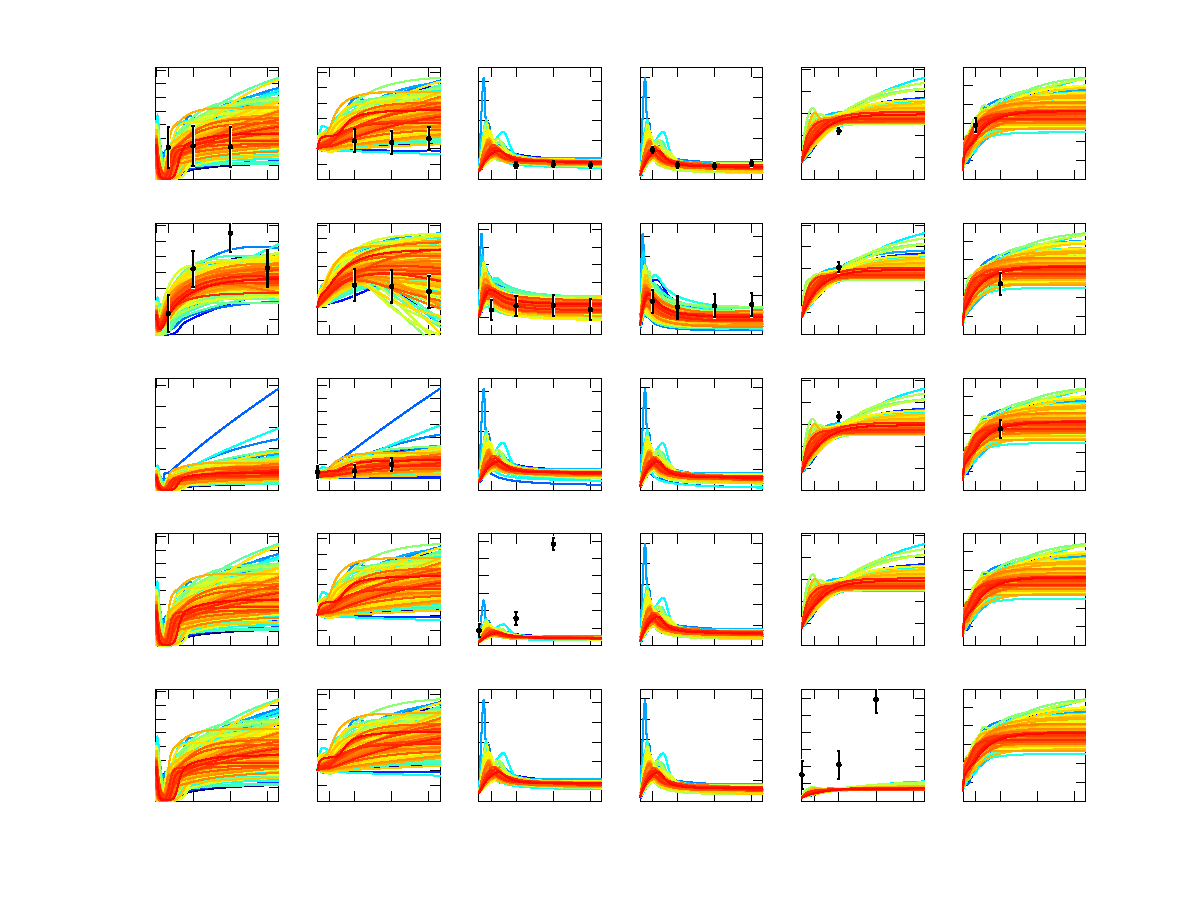
\includegraphics{SampleOutputs}}%
    \gplfronttext
  \end{picture}%
\endgroup
};
    \node (Ytitle) at (plot.north) {model outputs};
    \foreach \i in {1,...,6} \node (Ylabel\i) at (-9.25+2.75*\i,7) {$y_\i$};
    \node (Tlabel) at (plot.south) {time $t$ in h};
    \node (Tdescription) [above of=Tlabel] {measurements were taken at $\{0.1,\,8,\,24,\,48,\,72\}$ h};
    \node (Utitle) at (-9,0) [rotate=90]{experiment conditions (inputs)};
    \foreach \i in {0,...,4} \node (Ulabel\i) at (-8.5,5.6-2.66*\i) {$u_\i$};
  \end{tikzpicture}
  \caption{Treating the data as absolute, the fit changes ($u_0$ is
    the setup for the reference experiment). Some data points get an
    improved fit, some system behaviour cannot be reproduced. Note
    that this treatment of the data is incorrect and is done for
    illustration purposes; we show the difference between fitting
    absolute and relative data. To obtain these Trajectories, we have
    used a different, uninformative, iid, Gaussian prior during
    sampling. The resulting parameter sample is shown in
    Figure~\ref{fig:AbsoluteSample}}
  \label{fig:AbsoluteFit}
\end{figure}

\begin{figure}
  \centering 
  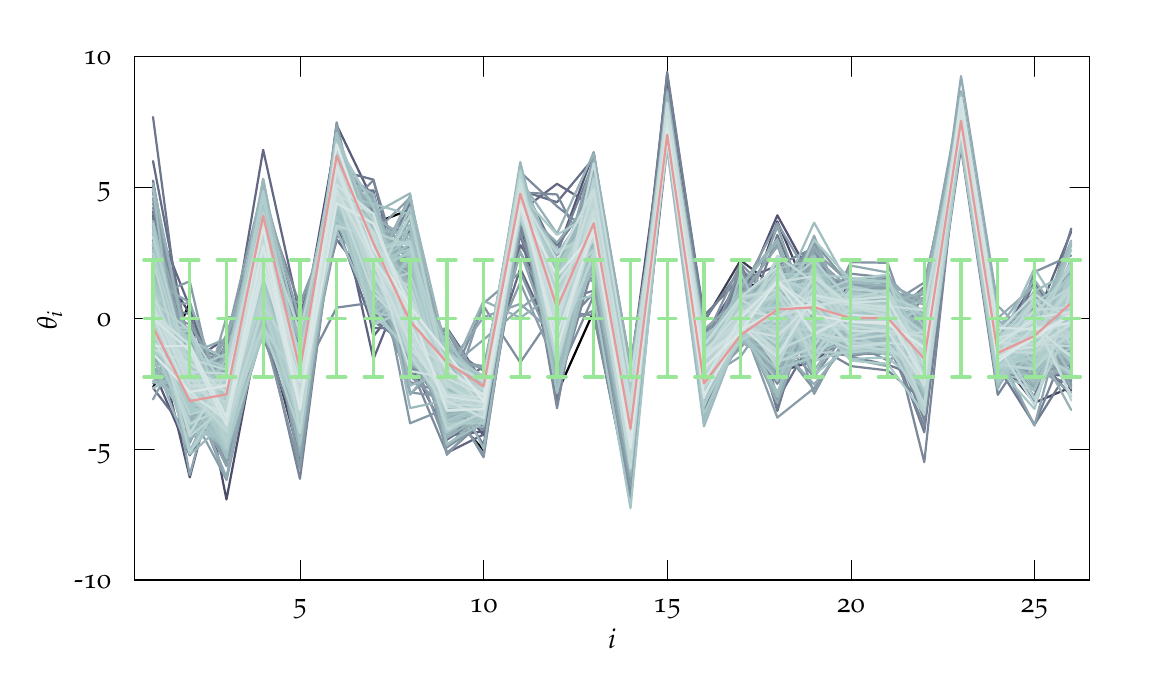
\begin{tikzpicture}[gnuplot]
%% generated with GNUPLOT 4.6p1 (Gentoo revision r0) (Lua 5.1; terminal rev. 99, script rev. 100)
%% Mi 31 Jul 2013 18:59:20 CEST
\path (0.000,0.000) rectangle (14.000,8.000);
\gpfill{rgb color={1.000,1.000,1.000}} (1.320,0.985)--(13.446,0.985)--(13.446,7.630)--(1.320,7.630)--cycle;
\gpcolor{color=gp lt color border}
\gpsetlinetype{gp lt border}
\gpsetlinewidth{1.00}
\draw[gp path] (1.320,0.985)--(1.320,7.630)--(13.446,7.630)--(13.446,0.985)--cycle;
\gpsetlinewidth{0.50}
\draw[gp path] (1.320,0.985)--(1.571,0.985);
\draw[gp path] (13.447,0.985)--(13.196,0.985);
\gpcolor{rgb color={0.000,0.000,0.000}}
\node[gp node right,font={\fontsize{10pt}{12pt}\selectfont}] at (1.136,0.985) {-10};
\gpcolor{color=gp lt color border}
\draw[gp path] (1.320,2.647)--(1.571,2.647);
\draw[gp path] (13.447,2.647)--(13.196,2.647);
\gpcolor{rgb color={0.000,0.000,0.000}}
\node[gp node right,font={\fontsize{10pt}{12pt}\selectfont}] at (1.136,2.647) {-5};
\gpcolor{color=gp lt color border}
\draw[gp path] (1.320,4.308)--(1.571,4.308);
\draw[gp path] (13.447,4.308)--(13.196,4.308);
\gpcolor{rgb color={0.000,0.000,0.000}}
\node[gp node right,font={\fontsize{10pt}{12pt}\selectfont}] at (1.136,4.308) {0};
\gpcolor{color=gp lt color border}
\draw[gp path] (1.320,5.970)--(1.571,5.970);
\draw[gp path] (13.447,5.970)--(13.196,5.970);
\gpcolor{rgb color={0.000,0.000,0.000}}
\node[gp node right,font={\fontsize{10pt}{12pt}\selectfont}] at (1.136,5.970) {5};
\gpcolor{color=gp lt color border}
\draw[gp path] (1.320,7.631)--(1.571,7.631);
\draw[gp path] (13.447,7.631)--(13.196,7.631);
\gpcolor{rgb color={0.000,0.000,0.000}}
\node[gp node right,font={\fontsize{10pt}{12pt}\selectfont}] at (1.136,7.631) {10};
\gpcolor{color=gp lt color border}
\draw[gp path] (3.419,0.985)--(3.419,1.236);
\draw[gp path] (3.419,7.631)--(3.419,7.380);
\gpcolor{rgb color={0.000,0.000,0.000}}
\node[gp node center,font={\fontsize{10pt}{12pt}\selectfont}] at (3.419,0.677) {5};
\gpcolor{color=gp lt color border}
\draw[gp path] (5.751,0.985)--(5.751,1.236);
\draw[gp path] (5.751,7.631)--(5.751,7.380);
\gpcolor{rgb color={0.000,0.000,0.000}}
\node[gp node center,font={\fontsize{10pt}{12pt}\selectfont}] at (5.751,0.677) {10};
\gpcolor{color=gp lt color border}
\draw[gp path] (8.083,0.985)--(8.083,1.236);
\draw[gp path] (8.083,7.631)--(8.083,7.380);
\gpcolor{rgb color={0.000,0.000,0.000}}
\node[gp node center,font={\fontsize{10pt}{12pt}\selectfont}] at (8.083,0.677) {15};
\gpcolor{color=gp lt color border}
\draw[gp path] (10.415,0.985)--(10.415,1.236);
\draw[gp path] (10.415,7.631)--(10.415,7.380);
\gpcolor{rgb color={0.000,0.000,0.000}}
\node[gp node center,font={\fontsize{10pt}{12pt}\selectfont}] at (10.415,0.677) {20};
\gpcolor{color=gp lt color border}
\draw[gp path] (12.747,0.985)--(12.747,1.236);
\draw[gp path] (12.747,7.631)--(12.747,7.380);
\gpcolor{rgb color={0.000,0.000,0.000}}
\node[gp node center,font={\fontsize{10pt}{12pt}\selectfont}] at (12.747,0.677) {25};
\gpcolor{color=gp lt color border}
\draw[gp path] (1.320,7.631)--(1.320,0.985)--(13.447,0.985)--(13.447,7.631)--cycle;
\gpcolor{rgb color={0.000,0.000,0.000}}
\node[gp node center,rotate=90,font={\fontsize{10pt}{12pt}\selectfont}] at (0.246,4.308) {$\theta_i$};
\node[gp node center,font={\fontsize{10pt}{12pt}\selectfont}] at (7.383,0.215) {$i$};
\gpsetlinetype{gp lt plot 0}
\gpsetlinewidth{2.00}
\draw[gp path] (1.553,3.426)--(2.020,4.508)--(2.486,2.859)--(2.952,5.427)--(3.419,4.009)%
  --(3.885,5.767)--(4.352,5.509)--(4.818,5.692)--(5.285,3.156)--(5.751,2.635)--(6.217,5.547)%
  --(6.684,3.354)--(7.150,4.398)--(7.617,2.055)--(8.083,7.162)--(8.550,3.545)--(9.016,4.713)%
  --(9.482,4.764)--(9.949,4.088)--(10.415,4.037)--(10.882,3.973)--(11.348,4.283)--(11.815,6.974)%
  --(12.281,4.079)--(12.747,3.605)--(13.214,4.583);
\gpcolor{rgb color={0.239,0.239,0.329}}
\draw[gp path] (1.553,5.925)--(2.020,3.274)--(2.486,3.225)--(2.952,4.702)--(3.419,4.099)%
  --(3.885,5.402)--(4.352,5.444)--(4.818,4.850)--(5.285,2.828)--(5.751,3.084)--(6.217,5.982)%
  --(6.684,4.004)--(7.150,5.691)--(7.617,3.029)--(8.083,7.352)--(8.550,4.261)--(9.016,5.046)%
  --(9.482,4.686)--(9.949,5.139)--(10.415,4.302)--(10.882,4.410)--(11.348,4.361)--(11.815,6.749)%
  --(12.281,3.736)--(12.747,4.082)--(13.214,4.741);
\gpcolor{rgb color={0.275,0.275,0.376}}
\draw[gp path] (1.553,3.981)--(2.020,4.097)--(2.486,2.750)--(2.952,4.282)--(3.419,2.537)%
  --(3.885,6.070)--(4.352,4.951)--(4.818,4.538)--(5.285,3.527)--(5.751,2.908)--(6.217,5.703)%
  --(6.684,4.126)--(7.150,5.931)--(7.617,3.426)--(8.083,6.762)--(8.550,3.577)--(9.016,4.212)%
  --(9.482,5.539)--(9.949,4.443)--(10.415,4.801)--(10.882,4.808)--(11.348,3.159)--(11.815,6.743)%
  --(12.281,3.811)--(12.747,3.237)--(13.214,3.434);
\gpcolor{rgb color={0.302,0.302,0.416}}
\draw[gp path] (1.553,5.114)--(2.020,4.367)--(2.486,2.008)--(2.952,4.465)--(3.419,3.548)%
  --(3.885,6.364)--(4.352,5.111)--(4.818,4.802)--(5.285,3.739)--(5.751,3.120)--(6.217,5.832)%
  --(6.684,3.634)--(7.150,5.280)--(7.617,2.782)--(8.083,7.009)--(8.550,3.101)--(9.016,4.511)%
  --(9.482,3.623)--(9.949,3.768)--(10.415,4.106)--(10.882,4.043)--(11.348,3.423)--(11.815,6.900)%
  --(12.281,3.989)--(12.747,3.683)--(13.214,4.466);
\gpcolor{rgb color={0.318,0.318,0.439}}
\draw[gp path] (1.553,4.240)--(2.020,2.289)--(2.486,4.048)--(2.952,4.581)--(3.419,3.733)%
  --(3.885,6.004)--(4.352,5.010)--(4.818,4.319)--(5.285,3.417)--(5.751,2.823)--(6.217,5.482)%
  --(6.684,5.138)--(7.150,6.417)--(7.617,3.457)--(8.083,6.679)--(8.550,3.278)--(9.016,4.340)%
  --(9.482,3.616)--(9.949,4.296)--(10.415,3.954)--(10.882,4.013)--(11.348,3.177)--(11.815,6.690)%
  --(12.281,3.689)--(12.747,3.795)--(13.214,4.511);
\gpcolor{rgb color={0.325,0.325,0.451}}
\draw[gp path] (1.553,5.385)--(2.020,3.354)--(2.486,3.363)--(2.952,5.907)--(3.419,4.004)%
  --(3.885,6.639)--(4.352,4.294)--(4.818,4.367)--(5.285,4.080)--(5.751,3.088)--(6.217,5.795)%
  --(6.684,4.366)--(7.150,6.354)--(7.617,3.667)--(8.083,7.103)--(8.550,3.852)--(9.016,4.530)%
  --(9.482,5.617)--(9.949,4.768)--(10.415,4.346)--(10.882,4.417)--(11.348,3.805)--(11.815,6.816)%
  --(12.281,3.854)--(12.747,3.556)--(13.214,4.368);
\gpcolor{rgb color={0.337,0.337,0.463}}
\draw[gp path] (1.553,3.659)--(2.020,2.570)--(2.486,3.312)--(2.952,5.132)--(3.419,3.536)%
  --(3.885,5.919)--(4.352,5.052)--(4.818,4.087)--(5.285,3.330)--(5.751,3.076)--(6.217,5.865)%
  --(6.684,4.238)--(7.150,5.979)--(7.617,2.735)--(8.083,6.837)--(8.550,3.990)--(9.016,4.207)%
  --(9.482,3.510)--(9.949,4.151)--(10.415,4.129)--(10.882,4.051)--(11.348,4.256)--(11.815,7.066)%
  --(12.281,4.167)--(12.747,4.233)--(13.214,4.921);
\gpcolor{rgb color={0.353,0.365,0.478}}
\draw[gp path] (1.553,5.664)--(2.020,3.626)--(2.486,3.347)--(2.952,4.643)--(3.419,3.309)%
  --(3.885,6.765)--(4.352,5.795)--(4.818,3.937)--(5.285,4.189)--(5.751,3.488)--(6.217,5.874)%
  --(6.684,4.007)--(7.150,5.998)--(7.617,3.273)--(8.083,6.877)--(8.550,3.788)--(9.016,4.415)%
  --(9.482,4.345)--(9.949,3.865)--(10.415,4.813)--(10.882,4.622)--(11.348,4.551)--(11.815,7.025)%
  --(12.281,4.192)--(12.747,4.535)--(13.214,3.392);
\draw[gp path] (1.553,4.540)--(2.020,3.436)--(2.486,3.915)--(2.952,4.734)--(3.419,3.158)%
  --(3.885,5.400)--(4.352,5.291)--(4.818,3.745)--(5.285,2.820)--(5.751,2.871)--(6.217,5.614)%
  --(6.684,4.819)--(7.150,6.014)--(7.617,3.068)--(8.083,7.128)--(8.550,4.077)--(9.016,4.800)%
  --(9.482,4.440)--(9.949,4.107)--(10.415,4.378)--(10.882,4.374)--(11.348,3.298)--(11.815,6.660)%
  --(12.281,3.672)--(12.747,3.871)--(13.214,3.322);
\gpcolor{rgb color={0.361,0.376,0.486}}
\draw[gp path] (1.553,5.989)--(2.020,3.752)--(2.486,4.055)--(2.952,5.608)--(3.419,3.014)%
  --(3.885,6.330)--(4.352,4.080)--(4.818,4.674)--(5.285,3.844)--(5.751,3.364)--(6.217,6.036)%
  --(6.684,3.794)--(7.150,6.027)--(7.617,3.256)--(8.083,6.844)--(8.550,3.745)--(9.016,4.276)%
  --(9.482,3.998)--(9.949,4.499)--(10.415,4.803)--(10.882,4.789)--(11.348,3.840)--(11.815,7.113)%
  --(12.281,4.215)--(12.747,3.751)--(13.214,4.843);
\gpcolor{rgb color={0.373,0.388,0.498}}
\draw[gp path] (1.553,4.076)--(2.020,4.111)--(2.486,3.449)--(2.952,5.848)--(3.419,3.010)%
  --(3.885,5.906)--(4.352,3.791)--(4.818,4.950)--(5.285,3.382)--(5.751,3.298)--(6.217,5.835)%
  --(6.684,4.213)--(7.150,6.012)--(7.617,3.192)--(8.083,7.130)--(8.550,3.972)--(9.016,4.786)%
  --(9.482,4.977)--(9.949,4.235)--(10.415,4.170)--(10.882,4.190)--(11.348,3.501)--(11.815,7.009)%
  --(12.281,4.045)--(12.747,4.761)--(13.214,3.858);
\gpcolor{rgb color={0.380,0.400,0.506}}
\draw[gp path] (1.553,5.938)--(2.020,3.118)--(2.486,3.359)--(2.952,4.283)--(3.419,3.262)%
  --(3.885,5.846)--(4.352,5.090)--(4.818,4.583)--(5.285,3.086)--(5.751,3.250)--(6.217,5.967)%
  --(6.684,3.427)--(7.150,5.602)--(7.617,2.912)--(8.083,6.823)--(8.550,3.669)--(9.016,4.547)%
  --(9.482,4.450)--(9.949,4.375)--(10.415,4.447)--(10.882,4.405)--(11.348,4.286)--(11.815,7.133)%
  --(12.281,4.234)--(12.747,4.260)--(13.214,5.409);
\draw[gp path] (1.553,5.618)--(2.020,4.451)--(2.486,3.083)--(2.952,5.719)--(3.419,3.723)%
  --(3.885,5.309)--(4.352,4.701)--(4.818,4.578)--(5.285,2.600)--(5.751,2.833)--(6.217,5.665)%
  --(6.684,6.017)--(7.150,5.728)--(7.617,2.713)--(8.083,6.935)--(8.550,3.770)--(9.016,4.739)%
  --(9.482,4.630)--(9.949,4.480)--(10.415,4.396)--(10.882,4.453)--(11.348,4.176)--(11.815,6.656)%
  --(12.281,3.674)--(12.747,3.400)--(13.214,4.152);
\gpcolor{rgb color={0.388,0.412,0.514}}
\draw[gp path] (1.553,4.419)--(2.020,2.837)--(2.486,3.702)--(2.952,6.449)--(3.419,4.343)%
  --(3.885,5.865)--(4.352,4.676)--(4.818,3.808)--(5.285,3.111)--(5.751,3.223)--(6.217,5.239)%
  --(6.684,4.546)--(7.150,6.078)--(7.617,3.318)--(8.083,6.612)--(8.550,3.622)--(9.016,4.061)%
  --(9.482,4.895)--(9.949,4.055)--(10.415,4.340)--(10.882,4.272)--(11.348,3.648)--(11.815,6.871)%
  --(12.281,3.969)--(12.747,3.310)--(13.214,4.892);
\draw[gp path] (1.553,4.635)--(2.020,3.466)--(2.486,3.590)--(2.952,4.933)--(3.419,2.411)%
  --(3.885,6.174)--(4.352,4.243)--(4.818,4.212)--(5.285,3.556)--(5.751,3.509)--(6.217,4.940)%
  --(6.684,3.940)--(7.150,5.436)--(7.617,2.793)--(8.083,6.643)--(8.550,3.627)--(9.016,4.137)%
  --(9.482,4.557)--(9.949,4.681)--(10.415,4.178)--(10.882,4.148)--(11.348,3.253)--(11.815,6.591)%
  --(12.281,3.607)--(12.747,3.902)--(13.214,3.766);
\gpcolor{rgb color={0.396,0.424,0.522}}
\draw[gp path] (1.553,6.306)--(2.020,3.863)--(2.486,3.788)--(2.952,5.594)--(3.419,3.331)%
  --(3.885,6.353)--(4.352,4.532)--(4.818,5.164)--(5.285,3.731)--(5.751,3.248)--(6.217,5.870)%
  --(6.684,3.780)--(7.150,5.509)--(7.617,3.201)--(8.083,7.074)--(8.550,3.774)--(9.016,4.422)%
  --(9.482,3.319)--(9.949,4.684)--(10.415,4.257)--(10.882,4.237)--(11.348,3.909)--(11.815,6.646)%
  --(12.281,3.667)--(12.747,4.030)--(13.214,3.909);
\draw[gp path] (1.553,5.615)--(2.020,3.276)--(2.486,3.574)--(2.952,5.389)--(3.419,3.222)%
  --(3.885,5.498)--(4.352,4.187)--(4.818,4.184)--(5.285,2.766)--(5.751,3.071)--(6.217,6.068)%
  --(6.684,5.115)--(7.150,5.468)--(7.617,3.132)--(8.083,6.812)--(8.550,3.637)--(9.016,4.232)%
  --(9.482,4.088)--(9.949,5.094)--(10.415,4.082)--(10.882,3.970)--(11.348,3.708)--(11.815,6.932)%
  --(12.281,4.048)--(12.747,3.608)--(13.214,3.574);
\gpcolor{rgb color={0.408,0.435,0.533}}
\draw[gp path] (1.553,4.369)--(2.020,3.700)--(2.486,3.858)--(2.952,5.018)--(3.419,3.210)%
  --(3.885,5.928)--(4.352,5.932)--(4.818,3.793)--(5.285,3.299)--(5.751,3.181)--(6.217,5.935)%
  --(6.684,5.783)--(7.150,6.344)--(7.617,3.218)--(8.083,6.845)--(8.550,3.875)--(9.016,4.442)%
  --(9.482,3.272)--(9.949,4.080)--(10.415,4.665)--(10.882,4.679)--(11.348,3.799)--(11.815,6.794)%
  --(12.281,3.841)--(12.747,3.548)--(13.214,4.742);
\draw[gp path] (1.553,4.815)--(2.020,2.729)--(2.486,3.801)--(2.952,5.539)--(3.419,3.073)%
  --(3.885,6.089)--(4.352,4.330)--(4.818,4.519)--(5.285,3.379)--(5.751,3.697)--(6.217,5.409)%
  --(6.684,4.875)--(7.150,5.599)--(7.617,2.757)--(8.083,6.678)--(8.550,3.797)--(9.016,4.165)%
  --(9.482,4.059)--(9.949,4.186)--(10.415,4.064)--(10.882,4.101)--(11.348,4.248)--(11.815,6.873)%
  --(12.281,3.929)--(12.747,3.628)--(13.214,5.061);
\gpcolor{rgb color={0.416,0.447,0.541}}
\draw[gp path] (1.553,4.415)--(2.020,3.975)--(2.486,3.246)--(2.952,4.835)--(3.419,4.015)%
  --(3.885,6.132)--(4.352,4.827)--(4.818,5.600)--(5.285,3.643)--(5.751,3.268)--(6.217,5.862)%
  --(6.684,3.239)--(7.150,5.608)--(7.617,2.758)--(8.083,7.104)--(8.550,3.680)--(9.016,4.742)%
  --(9.482,4.479)--(9.949,3.799)--(10.415,4.168)--(10.882,4.317)--(11.348,3.234)--(11.815,6.804)%
  --(12.281,3.774)--(12.747,3.873)--(13.214,3.742);
\draw[gp path] (1.553,5.569)--(2.020,3.063)--(2.486,3.291)--(2.952,4.464)--(3.419,3.405)%
  --(3.885,6.630)--(4.352,4.625)--(4.818,5.433)--(5.285,3.950)--(5.751,3.644)--(6.217,5.943)%
  --(6.684,4.532)--(7.150,5.190)--(7.617,2.307)--(8.083,6.492)--(8.550,3.114)--(9.016,4.126)%
  --(9.482,4.878)--(9.949,4.258)--(10.415,4.341)--(10.882,4.385)--(11.348,3.954)--(11.815,7.079)%
  --(12.281,4.141)--(12.747,4.195)--(13.214,4.379);
\draw[gp path] (1.553,3.425)--(2.020,2.817)--(2.486,3.025)--(2.952,5.539)--(3.419,3.902)%
  --(3.885,6.093)--(4.352,5.259)--(4.818,4.125)--(5.285,3.425)--(5.751,2.702)--(6.217,5.384)%
  --(6.684,3.555)--(7.150,5.448)--(7.617,2.734)--(8.083,6.851)--(8.550,3.900)--(9.016,4.221)%
  --(9.482,3.821)--(9.949,3.905)--(10.415,4.118)--(10.882,3.980)--(11.348,4.019)--(11.815,6.791)%
  --(12.281,3.899)--(12.747,4.773)--(13.214,4.172);
\gpcolor{rgb color={0.424,0.463,0.549}}
\draw[gp path] (1.553,6.865)--(2.020,3.342)--(2.486,3.917)--(2.952,4.287)--(3.419,3.552)%
  --(3.885,5.879)--(4.352,4.849)--(4.818,4.096)--(5.285,3.111)--(5.751,3.308)--(6.217,5.934)%
  --(6.684,4.109)--(7.150,6.262)--(7.617,3.404)--(8.083,6.787)--(8.550,3.825)--(9.016,4.401)%
  --(9.482,4.193)--(9.949,4.322)--(10.415,4.163)--(10.882,4.110)--(11.348,4.121)--(11.815,6.616)%
  --(12.281,3.658)--(12.747,4.145)--(13.214,3.586);
\draw[gp path] (1.553,5.012)--(2.020,2.877)--(2.486,3.473)--(2.952,5.801)--(3.419,4.196)%
  --(3.885,5.998)--(4.352,4.632)--(4.818,4.453)--(5.285,3.328)--(5.751,3.333)--(6.217,5.828)%
  --(6.684,4.750)--(7.150,5.702)--(7.617,3.196)--(8.083,7.407)--(8.550,3.562)--(9.016,4.983)%
  --(9.482,4.094)--(9.949,4.055)--(10.415,4.153)--(10.882,4.153)--(11.348,3.601)--(11.815,6.685)%
  --(12.281,3.696)--(12.747,4.784)--(13.214,3.924);
\draw[gp path] (1.553,4.331)--(2.020,3.774)--(2.486,3.764)--(2.952,5.138)--(3.419,3.754)%
  --(3.885,6.193)--(4.352,6.070)--(4.818,4.166)--(5.285,3.566)--(5.751,3.338)--(6.217,5.806)%
  --(6.684,4.796)--(7.150,5.886)--(7.617,3.208)--(8.083,7.382)--(8.550,4.342)--(9.016,4.825)%
  --(9.482,3.313)--(9.949,4.522)--(10.415,4.431)--(10.882,4.473)--(11.348,3.180)--(11.815,6.667)%
  --(12.281,3.443)--(12.747,4.502)--(13.214,4.002);
\gpcolor{rgb color={0.431,0.475,0.557}}
\draw[gp path] (1.553,4.067)--(2.020,3.351)--(2.486,3.250)--(2.952,4.729)--(3.419,2.733)%
  --(3.885,6.194)--(4.352,4.917)--(4.818,4.618)--(5.285,3.504)--(5.751,3.197)--(6.217,5.812)%
  --(6.684,5.233)--(7.150,5.860)--(7.617,3.096)--(8.083,7.124)--(8.550,4.088)--(9.016,4.485)%
  --(9.482,4.237)--(9.949,5.282)--(10.415,4.014)--(10.882,4.038)--(11.348,3.855)--(11.815,6.803)%
  --(12.281,3.856)--(12.747,3.956)--(13.214,3.523);
\draw[gp path] (1.553,4.459)--(2.020,4.364)--(2.486,2.963)--(2.952,5.303)--(3.419,3.582)%
  --(3.885,6.195)--(4.352,5.890)--(4.818,4.104)--(5.285,3.774)--(5.751,3.053)--(6.217,5.745)%
  --(6.684,4.084)--(7.150,5.578)--(7.617,2.611)--(8.083,7.069)--(8.550,3.938)--(9.016,4.730)%
  --(9.482,3.132)--(9.949,4.691)--(10.415,4.707)--(10.882,4.705)--(11.348,4.051)--(11.815,6.823)%
  --(12.281,3.874)--(12.747,4.121)--(13.214,4.047);
\draw[gp path] (1.553,4.177)--(2.020,2.612)--(2.486,3.619)--(2.952,4.391)--(3.419,3.619)%
  --(3.885,5.483)--(4.352,5.658)--(4.818,4.525)--(5.285,2.828)--(5.751,3.035)--(6.217,5.913)%
  --(6.684,4.804)--(7.150,6.174)--(7.617,3.592)--(8.083,6.712)--(8.550,3.770)--(9.016,4.074)%
  --(9.482,5.367)--(9.949,4.247)--(10.415,3.819)--(10.882,3.721)--(11.348,3.541)--(11.815,6.829)%
  --(12.281,3.915)--(12.747,3.941)--(13.214,4.036);
\draw[gp path] (1.553,4.982)--(2.020,3.640)--(2.486,2.714)--(2.952,4.813)--(3.419,3.025)%
  --(3.885,5.638)--(4.352,5.119)--(4.818,4.609)--(5.285,2.846)--(5.751,3.119)--(6.217,5.993)%
  --(6.684,4.919)--(7.150,5.173)--(7.617,2.644)--(8.083,6.888)--(8.550,3.803)--(9.016,4.385)%
  --(9.482,3.681)--(9.949,4.412)--(10.415,4.153)--(10.882,4.117)--(11.348,4.365)--(11.815,6.676)%
  --(12.281,3.697)--(12.747,2.958)--(13.214,3.701);
\gpcolor{rgb color={0.443,0.486,0.569}}
\draw[gp path] (1.553,4.035)--(2.020,3.189)--(2.486,3.982)--(2.952,5.071)--(3.419,3.185)%
  --(3.885,6.430)--(4.352,5.613)--(4.818,4.489)--(5.285,3.818)--(5.751,3.553)--(6.217,6.157)%
  --(6.684,3.339)--(7.150,5.689)--(7.617,2.791)--(8.083,6.574)--(8.550,3.294)--(9.016,4.107)%
  --(9.482,4.294)--(9.949,4.767)--(10.415,4.066)--(10.882,4.143)--(11.348,3.831)--(11.815,6.906)%
  --(12.281,3.938)--(12.747,4.423)--(13.214,4.030);
\draw[gp path] (1.553,5.101)--(2.020,3.296)--(2.486,3.224)--(2.952,4.714)--(3.419,3.998)%
  --(3.885,6.067)--(4.352,5.232)--(4.818,5.200)--(5.285,3.551)--(5.751,2.993)--(6.217,5.485)%
  --(6.684,4.355)--(7.150,5.459)--(7.617,2.694)--(8.083,6.946)--(8.550,3.759)--(9.016,4.429)%
  --(9.482,4.516)--(9.949,4.734)--(10.415,4.790)--(10.882,4.811)--(11.348,3.778)--(11.815,6.913)%
  --(12.281,3.989)--(12.747,3.649)--(13.214,4.517);
\draw[gp path] (1.553,6.058)--(2.020,3.467)--(2.486,3.459)--(2.952,4.934)--(3.419,3.140)%
  --(3.885,6.272)--(4.352,4.643)--(4.818,4.292)--(5.285,3.597)--(5.751,3.252)--(6.217,5.821)%
  --(6.684,3.647)--(7.150,5.604)--(7.617,3.114)--(8.083,7.075)--(8.550,4.154)--(9.016,4.457)%
  --(9.482,4.008)--(9.949,4.476)--(10.415,4.128)--(10.882,4.220)--(11.348,4.247)--(11.815,6.889)%
  --(12.281,3.925)--(12.747,3.905)--(13.214,5.448);
\gpcolor{rgb color={0.451,0.498,0.576}}
\draw[gp path] (1.553,4.148)--(2.020,2.997)--(2.486,3.399)--(2.952,4.836)--(3.419,3.502)%
  --(3.885,5.920)--(4.352,5.496)--(4.818,3.872)--(5.285,3.246)--(5.751,3.249)--(6.217,6.101)%
  --(6.684,4.908)--(7.150,6.119)--(7.617,3.355)--(8.083,6.879)--(8.550,3.877)--(9.016,4.438)%
  --(9.482,3.944)--(9.949,4.278)--(10.415,4.560)--(10.882,4.414)--(11.348,3.441)--(11.815,6.576)%
  --(12.281,3.632)--(12.747,3.650)--(13.214,3.464);
\draw[gp path] (1.553,4.833)--(2.020,3.772)--(2.486,3.551)--(2.952,4.703)--(3.419,3.205)%
  --(3.885,5.538)--(4.352,4.598)--(4.818,5.792)--(5.285,3.084)--(5.751,3.116)--(6.217,5.791)%
  --(6.684,3.414)--(7.150,5.827)--(7.617,2.973)--(8.083,6.621)--(8.550,3.505)--(9.016,4.295)%
  --(9.482,4.150)--(9.949,4.519)--(10.415,4.509)--(10.882,4.350)--(11.348,3.654)--(11.815,6.972)%
  --(12.281,4.085)--(12.747,3.899)--(13.214,4.308);
\draw[gp path] (1.553,3.953)--(2.020,2.840)--(2.486,3.591)--(2.952,4.750)--(3.419,3.340)%
  --(3.885,6.108)--(4.352,5.054)--(4.818,5.651)--(5.285,3.418)--(5.751,3.342)--(6.217,5.972)%
  --(6.684,3.533)--(7.150,5.609)--(7.617,2.947)--(8.083,6.908)--(8.550,3.301)--(9.016,4.496)%
  --(9.482,3.205)--(9.949,4.963)--(10.415,4.344)--(10.882,4.249)--(11.348,4.380)--(11.815,6.952)%
  --(12.281,4.084)--(12.747,4.645)--(13.214,4.027);
\draw[gp path] (1.553,4.639)--(2.020,3.027)--(2.486,3.432)--(2.952,5.191)--(3.419,3.456)%
  --(3.885,5.895)--(4.352,4.268)--(4.818,3.964)--(5.285,3.247)--(5.751,3.047)--(6.217,5.780)%
  --(6.684,3.800)--(7.150,6.092)--(7.617,3.700)--(8.083,6.658)--(8.550,3.433)--(9.016,4.005)%
  --(9.482,4.684)--(9.949,4.254)--(10.415,4.135)--(10.882,4.137)--(11.348,2.862)--(11.815,6.692)%
  --(12.281,3.667)--(12.747,3.935)--(13.214,3.917);
\gpcolor{rgb color={0.459,0.510,0.584}}
\draw[gp path] (1.553,4.902)--(2.020,3.522)--(2.486,3.410)--(2.952,4.278)--(3.419,2.270)%
  --(3.885,5.846)--(4.352,5.130)--(4.818,5.691)--(5.285,3.051)--(5.751,3.149)--(6.217,5.766)%
  --(6.684,4.446)--(7.150,5.234)--(7.617,2.542)--(8.083,6.592)--(8.550,3.449)--(9.016,4.038)%
  --(9.482,4.090)--(9.949,4.120)--(10.415,4.324)--(10.882,4.284)--(11.348,4.711)--(11.815,6.909)%
  --(12.281,4.014)--(12.747,4.079)--(13.214,4.587);
\draw[gp path] (1.553,5.067)--(2.020,3.487)--(2.486,2.769)--(2.952,4.910)--(3.419,3.038)%
  --(3.885,5.883)--(4.352,4.376)--(4.818,4.811)--(5.285,3.231)--(5.751,3.022)--(6.217,5.797)%
  --(6.684,4.077)--(7.150,5.535)--(7.617,2.894)--(8.083,7.437)--(8.550,4.282)--(9.016,4.934)%
  --(9.482,4.518)--(9.949,4.216)--(10.415,4.335)--(10.882,4.265)--(11.348,3.898)--(11.815,6.871)%
  --(12.281,3.932)--(12.747,3.765)--(13.214,4.332);
\draw[gp path] (1.553,4.932)--(2.020,3.231)--(2.486,3.683)--(2.952,4.904)--(3.419,2.665)%
  --(3.885,5.696)--(4.352,4.757)--(4.818,3.802)--(5.285,3.090)--(5.751,3.136)--(6.217,5.898)%
  --(6.684,5.142)--(7.150,6.284)--(7.617,3.535)--(8.083,6.658)--(8.550,3.539)--(9.016,4.274)%
  --(9.482,4.002)--(9.949,4.364)--(10.415,4.145)--(10.882,4.384)--(11.348,4.167)--(11.815,6.656)%
  --(12.281,3.630)--(12.747,4.242)--(13.214,4.310);
\draw[gp path] (1.553,5.262)--(2.020,3.984)--(2.486,3.251)--(2.952,4.410)--(3.419,3.346)%
  --(3.885,5.548)--(4.352,5.316)--(4.818,4.481)--(5.285,3.087)--(5.751,3.132)--(6.217,5.979)%
  --(6.684,4.804)--(7.150,6.067)--(7.617,3.319)--(8.083,7.188)--(8.550,3.708)--(9.016,4.877)%
  --(9.482,4.206)--(9.949,4.020)--(10.415,4.183)--(10.882,4.164)--(11.348,3.397)--(11.815,6.665)%
  --(12.281,3.651)--(12.747,4.160)--(13.214,4.018);
\draw[gp path] (1.553,4.406)--(2.020,2.947)--(2.486,3.146)--(2.952,4.260)--(3.419,2.950)%
  --(3.885,6.263)--(4.352,4.412)--(4.818,5.008)--(5.285,3.585)--(5.751,3.533)--(6.217,6.043)%
  --(6.684,4.938)--(7.150,5.169)--(7.617,2.404)--(8.083,6.616)--(8.550,3.233)--(9.016,4.285)%
  --(9.482,4.406)--(9.949,4.813)--(10.415,4.600)--(10.882,4.696)--(11.348,3.538)--(11.815,6.898)%
  --(12.281,3.950)--(12.747,3.683)--(13.214,4.701);
\gpcolor{rgb color={0.467,0.522,0.592}}
\draw[gp path] (1.553,5.296)--(2.020,3.656)--(2.486,2.597)--(2.952,4.154)--(3.419,3.370)%
  --(3.885,6.573)--(4.352,5.369)--(4.818,4.631)--(5.285,3.977)--(5.751,3.548)--(6.217,6.220)%
  --(6.684,4.124)--(7.150,4.631)--(7.617,1.994)--(8.083,6.749)--(8.550,3.645)--(9.016,4.231)%
  --(9.482,4.625)--(9.949,4.667)--(10.415,3.856)--(10.882,3.860)--(11.348,4.054)--(11.815,6.906)%
  --(12.281,3.957)--(12.747,4.185)--(13.214,3.511);
\draw[gp path] (1.553,5.046)--(2.020,3.023)--(2.486,3.210)--(2.952,4.072)--(3.419,2.810)%
  --(3.885,6.031)--(4.352,5.686)--(4.818,4.526)--(5.285,3.401)--(5.751,3.259)--(6.217,6.092)%
  --(6.684,4.650)--(7.150,5.786)--(7.617,3.074)--(8.083,6.725)--(8.550,3.259)--(9.016,4.345)%
  --(9.482,5.034)--(9.949,4.324)--(10.415,4.086)--(10.882,4.001)--(11.348,4.584)--(11.815,6.839)%
  --(12.281,3.943)--(12.747,3.661)--(13.214,4.428);
\draw[gp path] (1.553,4.732)--(2.020,3.484)--(2.486,3.542)--(2.952,5.660)--(3.419,3.960)%
  --(3.885,5.655)--(4.352,5.675)--(4.818,4.848)--(5.285,3.143)--(5.751,2.910)--(6.217,5.817)%
  --(6.684,4.531)--(7.150,4.659)--(7.617,2.320)--(8.083,6.591)--(8.550,3.226)--(9.016,4.009)%
  --(9.482,3.765)--(9.949,3.950)--(10.415,4.021)--(10.882,4.063)--(11.348,4.099)--(11.815,6.822)%
  --(12.281,3.868)--(12.747,3.390)--(13.214,4.158);
\draw[gp path] (1.553,5.507)--(2.020,3.086)--(2.486,3.306)--(2.952,5.058)--(3.419,3.144)%
  --(3.885,6.145)--(4.352,4.378)--(4.818,5.256)--(5.285,3.586)--(5.751,3.380)--(6.217,6.006)%
  --(6.684,4.243)--(7.150,5.386)--(7.617,2.862)--(8.083,7.043)--(8.550,4.042)--(9.016,4.512)%
  --(9.482,3.993)--(9.949,4.096)--(10.415,4.209)--(10.882,4.228)--(11.348,4.260)--(11.815,6.798)%
  --(12.281,3.822)--(12.747,2.953)--(13.214,4.097);
\draw[gp path] (1.553,3.657)--(2.020,2.992)--(2.486,3.797)--(2.952,5.286)--(3.419,3.571)%
  --(3.885,5.669)--(4.352,5.223)--(4.818,4.386)--(5.285,3.155)--(5.751,3.056)--(6.217,5.970)%
  --(6.684,4.248)--(7.150,5.536)--(7.617,3.112)--(8.083,7.056)--(8.550,3.950)--(9.016,4.473)%
  --(9.482,4.605)--(9.949,3.972)--(10.415,3.702)--(10.882,3.647)--(11.348,3.254)--(11.815,6.474)%
  --(12.281,3.337)--(12.747,4.039)--(13.214,3.947);
\gpcolor{rgb color={0.478,0.533,0.604}}
\draw[gp path] (1.553,3.898)--(2.020,3.458)--(2.486,3.213)--(2.952,4.719)--(3.419,3.666)%
  --(3.885,5.479)--(4.352,4.979)--(4.818,4.594)--(5.285,2.961)--(5.751,3.175)--(6.217,6.030)%
  --(6.684,4.755)--(7.150,5.241)--(7.617,2.518)--(8.083,7.042)--(8.550,4.123)--(9.016,4.511)%
  --(9.482,4.980)--(9.949,5.203)--(10.415,4.023)--(10.882,3.998)--(11.348,2.946)--(11.815,6.903)%
  --(12.281,3.940)--(12.747,4.003)--(13.214,4.085);
\draw[gp path] (1.553,4.436)--(2.020,3.369)--(2.486,3.073)--(2.952,4.561)--(3.419,3.004)%
  --(3.885,6.144)--(4.352,4.835)--(4.818,3.566)--(5.285,3.543)--(5.751,3.487)--(6.217,6.143)%
  --(6.684,3.387)--(7.150,4.995)--(7.617,2.458)--(8.083,6.770)--(8.550,3.556)--(9.016,4.313)%
  --(9.482,3.998)--(9.949,4.059)--(10.415,4.220)--(10.882,4.171)--(11.348,3.021)--(11.815,7.005)%
  --(12.281,4.088)--(12.747,3.692)--(13.214,4.444);
\draw[gp path] (1.553,3.839)--(2.020,4.022)--(2.486,3.219)--(2.952,5.817)--(3.419,4.470)%
  --(3.885,5.591)--(4.352,6.063)--(4.818,4.525)--(5.285,2.791)--(5.751,3.042)--(6.217,5.708)%
  --(6.684,3.937)--(7.150,5.722)--(7.617,2.800)--(8.083,6.644)--(8.550,3.613)--(9.016,4.180)%
  --(9.482,4.025)--(9.949,3.841)--(10.415,4.327)--(10.882,4.262)--(11.348,3.867)--(11.815,7.011)%
  --(12.281,4.126)--(12.747,3.943)--(13.214,3.689);
\draw[gp path] (1.553,5.299)--(2.020,2.998)--(2.486,3.242)--(2.952,4.728)--(3.419,3.220)%
  --(3.885,5.858)--(4.352,4.945)--(4.818,4.189)--(5.285,3.090)--(5.751,3.031)--(6.217,5.464)%
  --(6.684,4.495)--(7.150,5.863)--(7.617,3.247)--(8.083,7.153)--(8.550,4.075)--(9.016,4.546)%
  --(9.482,4.534)--(9.949,4.735)--(10.415,4.177)--(10.882,4.014)--(11.348,4.212)--(11.815,6.702)%
  --(12.281,3.810)--(12.747,4.557)--(13.214,4.129);
\draw[gp path] (1.553,4.277)--(2.020,4.126)--(2.486,2.672)--(2.952,4.998)--(3.419,2.914)%
  --(3.885,5.895)--(4.352,4.788)--(4.818,4.615)--(5.285,3.181)--(5.751,2.891)--(6.217,5.598)%
  --(6.684,3.447)--(7.150,5.417)--(7.617,2.826)--(8.083,6.823)--(8.550,3.809)--(9.016,4.146)%
  --(9.482,3.478)--(9.949,4.171)--(10.415,4.263)--(10.882,4.339)--(11.348,3.693)--(11.815,6.678)%
  --(12.281,3.678)--(12.747,4.155)--(13.214,5.242);
\draw[gp path] (1.553,4.461)--(2.020,3.517)--(2.486,3.772)--(2.952,4.855)--(3.419,3.309)%
  --(3.885,6.528)--(4.352,4.624)--(4.818,4.055)--(5.285,3.887)--(5.751,3.150)--(6.217,5.609)%
  --(6.684,3.688)--(7.150,6.138)--(7.617,3.291)--(8.083,6.703)--(8.550,3.491)--(9.016,4.287)%
  --(9.482,4.992)--(9.949,4.837)--(10.415,4.239)--(10.882,4.347)--(11.348,2.482)--(11.815,6.851)%
  --(12.281,3.898)--(12.747,3.445)--(13.214,4.631);
\gpcolor{rgb color={0.486,0.545,0.612}}
\draw[gp path] (1.553,5.301)--(2.020,3.422)--(2.486,2.920)--(2.952,4.718)--(3.419,3.195)%
  --(3.885,6.295)--(4.352,4.327)--(4.818,4.895)--(5.285,3.708)--(5.751,3.575)--(6.217,6.083)%
  --(6.684,4.967)--(7.150,5.624)--(7.617,2.954)--(8.083,6.618)--(8.550,3.261)--(9.016,4.180)%
  --(9.482,4.229)--(9.949,4.366)--(10.415,4.105)--(10.882,4.042)--(11.348,3.631)--(11.815,6.652)%
  --(12.281,3.662)--(12.747,3.797)--(13.214,4.329);
\draw[gp path] (1.553,4.324)--(2.020,2.885)--(2.486,3.498)--(2.952,5.307)--(3.419,3.616)%
  --(3.885,5.294)--(4.352,5.240)--(4.818,4.995)--(5.285,2.669)--(5.751,2.996)--(6.217,5.829)%
  --(6.684,4.405)--(7.150,4.344)--(7.617,2.056)--(8.083,6.634)--(8.550,3.244)--(9.016,4.169)%
  --(9.482,4.415)--(9.949,3.779)--(10.415,4.517)--(10.882,4.409)--(11.348,4.212)--(11.815,6.897)%
  --(12.281,4.022)--(12.747,4.407)--(13.214,4.035);
\draw[gp path] (1.553,5.112)--(2.020,3.188)--(2.486,3.606)--(2.952,5.427)--(3.419,3.266)%
  --(3.885,6.290)--(4.352,4.319)--(4.818,4.267)--(5.285,3.741)--(5.751,3.392)--(6.217,5.879)%
  --(6.684,3.166)--(7.150,5.638)--(7.617,2.658)--(8.083,6.891)--(8.550,3.936)--(9.016,4.565)%
  --(9.482,4.008)--(9.949,4.321)--(10.415,4.403)--(10.882,4.330)--(11.348,3.996)--(11.815,6.753)%
  --(12.281,3.831)--(12.747,3.267)--(13.214,4.617);
\draw[gp path] (1.553,5.545)--(2.020,3.997)--(2.486,3.763)--(2.952,5.703)--(3.419,3.533)%
  --(3.885,4.445)--(4.352,4.509)--(4.818,3.702)--(5.285,2.595)--(5.751,3.008)--(6.217,5.909)%
  --(6.684,5.882)--(7.150,4.973)--(7.617,2.456)--(8.083,6.709)--(8.550,3.601)--(9.016,4.203)%
  --(9.482,4.742)--(9.949,5.258)--(10.415,4.063)--(10.882,4.004)--(11.348,3.369)--(11.815,6.648)%
  --(12.281,3.652)--(12.747,3.916)--(13.214,3.937);
\draw[gp path] (1.553,4.756)--(2.020,3.061)--(2.486,3.513)--(2.952,5.191)--(3.419,3.409)%
  --(3.885,6.302)--(4.352,4.422)--(4.818,4.619)--(5.285,3.817)--(5.751,3.171)--(6.217,5.661)%
  --(6.684,4.243)--(7.150,6.144)--(7.617,3.427)--(8.083,6.650)--(8.550,3.313)--(9.016,4.238)%
  --(9.482,4.999)--(9.949,3.864)--(10.415,4.216)--(10.882,4.319)--(11.348,3.637)--(11.815,6.977)%
  --(12.281,3.994)--(12.747,4.473)--(13.214,3.755);
\draw[gp path] (1.553,3.985)--(2.020,3.642)--(2.486,2.970)--(2.952,4.351)--(3.419,3.309)%
  --(3.885,6.115)--(4.352,5.650)--(4.818,4.254)--(5.285,3.483)--(5.751,3.431)--(6.217,6.166)%
  --(6.684,5.731)--(7.150,5.362)--(7.617,2.597)--(8.083,7.083)--(8.550,3.767)--(9.016,4.676)%
  --(9.482,4.522)--(9.949,4.747)--(10.415,4.019)--(10.882,4.040)--(11.348,3.322)--(11.815,6.641)%
  --(12.281,3.614)--(12.747,4.511)--(13.214,3.963);
\gpcolor{rgb color={0.494,0.557,0.620}}
\draw[gp path] (1.553,4.669)--(2.020,3.324)--(2.486,3.446)--(2.952,4.748)--(3.419,3.591)%
  --(3.885,6.329)--(4.352,5.414)--(4.818,3.828)--(5.285,3.778)--(5.751,3.425)--(6.217,5.962)%
  --(6.684,4.258)--(7.150,6.206)--(7.617,3.179)--(8.083,6.984)--(8.550,3.485)--(9.016,4.812)%
  --(9.482,4.238)--(9.949,3.898)--(10.415,3.829)--(10.882,3.904)--(11.348,3.747)--(11.815,6.616)%
  --(12.281,3.573)--(12.747,4.103)--(13.214,3.973);
\draw[gp path] (1.553,5.714)--(2.020,3.628)--(2.486,3.558)--(2.952,5.198)--(3.419,3.354)%
  --(3.885,5.700)--(4.352,4.278)--(4.818,4.656)--(5.285,3.081)--(5.751,3.190)--(6.217,5.864)%
  --(6.684,3.376)--(7.150,5.220)--(7.617,2.566)--(8.083,7.004)--(8.550,3.823)--(9.016,4.514)%
  --(9.482,4.035)--(9.949,4.278)--(10.415,4.875)--(10.882,4.827)--(11.348,3.643)--(11.815,6.718)%
  --(12.281,3.753)--(12.747,3.930)--(13.214,4.570);
\draw[gp path] (1.553,4.805)--(2.020,3.381)--(2.486,2.452)--(2.952,4.225)--(3.419,3.885)%
  --(3.885,6.050)--(4.352,5.724)--(4.818,5.071)--(5.285,3.460)--(5.751,3.366)--(6.217,5.862)%
  --(6.684,3.661)--(7.150,5.509)--(7.617,2.879)--(8.083,6.829)--(8.550,3.324)--(9.016,4.437)%
  --(9.482,4.384)--(9.949,4.450)--(10.415,4.232)--(10.882,4.208)--(11.348,4.222)--(11.815,6.788)%
  --(12.281,3.868)--(12.747,4.415)--(13.214,3.452);
\draw[gp path] (1.553,4.045)--(2.020,3.453)--(2.486,2.739)--(2.952,5.087)--(3.419,3.295)%
  --(3.885,6.061)--(4.352,5.621)--(4.818,3.818)--(5.285,3.330)--(5.751,3.090)--(6.217,5.393)%
  --(6.684,4.115)--(7.150,5.422)--(7.617,2.751)--(8.083,6.528)--(8.550,3.390)--(9.016,3.980)%
  --(9.482,4.777)--(9.949,4.301)--(10.415,4.482)--(10.882,4.340)--(11.348,4.092)--(11.815,7.039)%
  --(12.281,4.159)--(12.747,4.218)--(13.214,4.090);
\draw[gp path] (1.553,5.140)--(2.020,3.521)--(2.486,2.583)--(2.952,4.229)--(3.419,3.666)%
  --(3.885,6.026)--(4.352,5.643)--(4.818,4.999)--(5.285,3.397)--(5.751,4.464)--(6.217,3.748)%
  --(6.684,4.433)--(7.150,5.846)--(7.617,2.920)--(8.083,6.665)--(8.550,3.641)--(9.016,4.214)%
  --(9.482,4.408)--(9.949,3.988)--(10.415,4.267)--(10.882,4.161)--(11.348,4.421)--(11.815,6.881)%
  --(12.281,3.972)--(12.747,4.324)--(13.214,4.375);
\draw[gp path] (1.553,5.253)--(2.020,3.157)--(2.486,3.106)--(2.952,5.683)--(3.419,3.522)%
  --(3.885,5.844)--(4.352,4.682)--(4.818,3.499)--(5.285,3.357)--(5.751,3.111)--(6.217,5.853)%
  --(6.684,3.550)--(7.150,4.596)--(7.617,2.363)--(8.083,6.690)--(8.550,3.691)--(9.016,4.020)%
  --(9.482,4.211)--(9.949,4.431)--(10.415,4.235)--(10.882,4.242)--(11.348,4.382)--(11.815,6.748)%
  --(12.281,3.801)--(12.747,3.704)--(13.214,3.728);
\gpcolor{rgb color={0.502,0.573,0.627}}
\draw[gp path] (1.553,4.808)--(2.020,3.566)--(2.486,3.363)--(2.952,4.860)--(3.419,3.136)%
  --(3.885,6.075)--(4.352,5.633)--(4.818,4.022)--(5.285,3.361)--(5.751,3.369)--(6.217,6.053)%
  --(6.684,4.336)--(7.150,5.502)--(7.617,2.695)--(8.083,7.218)--(8.550,3.803)--(9.016,4.952)%
  --(9.482,3.897)--(9.949,4.580)--(10.415,4.183)--(10.882,4.297)--(11.348,4.180)--(11.815,6.785)%
  --(12.281,3.785)--(12.747,3.538)--(13.214,4.740);
\draw[gp path] (1.553,4.451)--(2.020,3.852)--(2.486,3.139)--(2.952,5.061)--(3.419,3.868)%
  --(3.885,5.708)--(4.352,5.557)--(4.818,4.709)--(5.285,3.075)--(5.751,3.000)--(6.217,5.739)%
  --(6.684,4.570)--(7.150,4.578)--(7.617,2.067)--(8.083,7.014)--(8.550,3.854)--(9.016,4.478)%
  --(9.482,4.092)--(9.949,3.563)--(10.415,4.219)--(10.882,4.322)--(11.348,3.577)--(11.815,6.621)%
  --(12.281,3.558)--(12.747,4.089)--(13.214,4.043);
\draw[gp path] (1.553,4.907)--(2.020,2.959)--(2.486,3.921)--(2.952,5.838)--(3.419,3.597)%
  --(3.885,6.061)--(4.352,4.553)--(4.818,3.781)--(5.285,3.575)--(5.751,3.298)--(6.217,5.964)%
  --(6.684,4.206)--(7.150,4.407)--(7.617,2.016)--(8.083,6.697)--(8.550,3.585)--(9.016,4.234)%
  --(9.482,4.743)--(9.949,4.819)--(10.415,4.370)--(10.882,4.410)--(11.348,3.623)--(11.815,6.740)%
  --(12.281,3.778)--(12.747,3.636)--(13.214,3.906);
\draw[gp path] (1.553,4.076)--(2.020,3.576)--(2.486,3.061)--(2.952,5.078)--(3.419,2.939)%
  --(3.885,6.403)--(4.352,5.153)--(4.818,4.367)--(5.285,3.784)--(5.751,2.992)--(6.217,5.666)%
  --(6.684,4.833)--(7.150,4.978)--(7.617,2.185)--(8.083,6.830)--(8.550,3.823)--(9.016,4.407)%
  --(9.482,4.553)--(9.949,4.043)--(10.415,3.996)--(10.882,3.774)--(11.348,4.005)--(11.815,6.883)%
  --(12.281,4.051)--(12.747,4.246)--(13.214,4.320);
\draw[gp path] (1.553,4.561)--(2.020,2.937)--(2.486,3.986)--(2.952,5.712)--(3.419,3.485)%
  --(3.885,6.508)--(4.352,4.684)--(4.818,4.290)--(5.285,3.974)--(5.751,3.367)--(6.217,5.883)%
  --(6.684,4.001)--(7.150,5.609)--(7.617,2.816)--(8.083,6.968)--(8.550,3.704)--(9.016,4.548)%
  --(9.482,4.336)--(9.949,5.241)--(10.415,4.308)--(10.882,4.336)--(11.348,3.685)--(11.815,6.684)%
  --(12.281,3.608)--(12.747,4.897)--(13.214,5.107);
\draw[gp path] (1.553,5.834)--(2.020,3.442)--(2.486,3.171)--(2.952,4.213)--(3.419,4.152)%
  --(3.885,5.850)--(4.352,5.274)--(4.818,3.714)--(5.285,3.325)--(5.751,2.544)--(6.217,5.666)%
  --(6.684,4.172)--(7.150,5.482)--(7.617,2.643)--(8.083,6.816)--(8.550,3.810)--(9.016,4.355)%
  --(9.482,3.695)--(9.949,4.258)--(10.415,4.192)--(10.882,4.201)--(11.348,3.585)--(11.815,6.710)%
  --(12.281,3.747)--(12.747,4.022)--(13.214,4.588);
\gpcolor{rgb color={0.514,0.584,0.639}}
\draw[gp path] (1.553,3.726)--(2.020,4.215)--(2.486,2.622)--(2.952,5.223)--(3.419,3.300)%
  --(3.885,6.082)--(4.352,5.337)--(4.818,4.017)--(5.285,3.359)--(5.751,3.453)--(6.217,6.106)%
  --(6.684,4.198)--(7.150,5.289)--(7.617,2.692)--(8.083,6.829)--(8.550,3.787)--(9.016,4.351)%
  --(9.482,4.293)--(9.949,4.947)--(10.415,3.897)--(10.882,4.056)--(11.348,3.274)--(11.815,6.690)%
  --(12.281,3.665)--(12.747,3.987)--(13.214,5.055);
\draw[gp path] (1.553,4.235)--(2.020,3.688)--(2.486,2.725)--(2.952,5.729)--(3.419,3.083)%
  --(3.885,5.360)--(4.352,5.005)--(4.818,3.918)--(5.285,2.686)--(5.751,3.006)--(6.217,5.825)%
  --(6.684,4.826)--(7.150,5.544)--(7.617,2.807)--(8.083,6.705)--(8.550,3.681)--(9.016,4.292)%
  --(9.482,4.589)--(9.949,5.276)--(10.415,4.709)--(10.882,4.669)--(11.348,4.518)--(11.815,6.685)%
  --(12.281,3.731)--(12.747,4.523)--(13.214,4.715);
\draw[gp path] (1.553,4.918)--(2.020,3.933)--(2.486,3.249)--(2.952,4.163)--(3.419,2.398)%
  --(3.885,6.370)--(4.352,5.171)--(4.818,4.474)--(5.285,3.766)--(5.751,3.372)--(6.217,5.819)%
  --(6.684,4.223)--(7.150,5.317)--(7.617,2.588)--(8.083,6.582)--(8.550,3.440)--(9.016,4.112)%
  --(9.482,3.997)--(9.949,3.405)--(10.415,4.122)--(10.882,4.192)--(11.348,3.638)--(11.815,6.834)%
  --(12.281,3.853)--(12.747,4.174)--(13.214,3.694);
\draw[gp path] (1.553,3.481)--(2.020,3.625)--(2.486,2.817)--(2.952,5.226)--(3.419,2.563)%
  --(3.885,6.511)--(4.352,4.971)--(4.818,4.383)--(5.285,3.850)--(5.751,3.268)--(6.217,5.725)%
  --(6.684,4.363)--(7.150,6.234)--(7.617,3.450)--(8.083,6.550)--(8.550,3.319)--(9.016,4.110)%
  --(9.482,4.769)--(9.949,4.555)--(10.415,4.107)--(10.882,3.952)--(11.348,4.298)--(11.815,6.991)%
  --(12.281,4.121)--(12.747,3.660)--(13.214,4.318);
\draw[gp path] (1.553,5.391)--(2.020,3.529)--(2.486,3.086)--(2.952,4.233)--(3.419,3.441)%
  --(3.885,5.988)--(4.352,4.849)--(4.818,4.316)--(5.285,3.284)--(5.751,3.418)--(6.217,5.152)%
  --(6.684,4.256)--(7.150,5.907)--(7.617,3.173)--(8.083,6.600)--(8.550,3.497)--(9.016,4.020)%
  --(9.482,4.852)--(9.949,4.920)--(10.415,4.710)--(10.882,4.796)--(11.348,3.380)--(11.815,6.906)%
  --(12.281,3.928)--(12.747,4.008)--(13.214,4.472);
\draw[gp path] (1.553,4.773)--(2.020,3.603)--(2.486,2.582)--(2.952,4.802)--(3.419,3.127)%
  --(3.885,6.798)--(4.352,4.727)--(4.818,4.155)--(5.285,4.148)--(5.751,3.327)--(6.217,5.779)%
  --(6.684,4.415)--(7.150,5.125)--(7.617,2.469)--(8.083,7.104)--(8.550,3.988)--(9.016,4.505)%
  --(9.482,3.785)--(9.949,4.374)--(10.415,4.121)--(10.882,4.116)--(11.348,3.798)--(11.815,6.666)%
  --(12.281,3.681)--(12.747,3.979)--(13.214,3.442);
\draw[gp path] (1.553,5.226)--(2.020,3.237)--(2.486,3.043)--(2.952,4.281)--(3.419,3.740)%
  --(3.885,6.353)--(4.352,4.917)--(4.818,4.873)--(5.285,3.726)--(5.751,3.334)--(6.217,5.826)%
  --(6.684,4.312)--(7.150,5.629)--(7.617,2.521)--(8.083,7.174)--(8.550,4.013)--(9.016,5.005)%
  --(9.482,4.514)--(9.949,4.030)--(10.415,5.021)--(10.882,5.014)--(11.348,3.688)--(11.815,6.976)%
  --(12.281,3.911)--(12.747,4.441)--(13.214,4.499);
\draw[gp path] (1.553,4.958)--(2.020,3.366)--(2.486,2.445)--(2.952,4.903)--(3.419,3.597)%
  --(3.885,5.604)--(4.352,5.108)--(4.818,4.415)--(5.285,3.101)--(5.751,2.998)--(6.217,5.816)%
  --(6.684,3.501)--(7.150,5.139)--(7.617,2.317)--(8.083,6.636)--(8.550,3.555)--(9.016,4.327)%
  --(9.482,4.335)--(9.949,4.227)--(10.415,4.490)--(10.882,4.469)--(11.348,4.763)--(11.815,6.763)%
  --(12.281,3.830)--(12.747,4.132)--(13.214,4.856);
\gpcolor{rgb color={0.522,0.596,0.647}}
\draw[gp path] (1.553,4.576)--(2.020,3.342)--(2.486,3.039)--(2.952,5.721)--(3.419,3.555)%
  --(3.885,5.775)--(4.352,5.533)--(4.818,3.869)--(5.285,3.276)--(5.751,2.576)--(6.217,5.553)%
  --(6.684,4.666)--(7.150,5.169)--(7.617,2.781)--(8.083,6.674)--(8.550,3.578)--(9.016,4.176)%
  --(9.482,3.814)--(9.949,4.030)--(10.415,4.364)--(10.882,4.389)--(11.348,4.570)--(11.815,6.860)%
  --(12.281,3.908)--(12.747,4.570)--(13.214,4.478);
\draw[gp path] (1.553,4.667)--(2.020,3.648)--(2.486,2.622)--(2.952,4.633)--(3.419,3.506)%
  --(3.885,5.912)--(4.352,5.291)--(4.818,4.587)--(5.285,3.334)--(5.751,3.054)--(6.217,5.790)%
  --(6.684,3.596)--(7.150,5.141)--(7.617,2.470)--(8.083,7.081)--(8.550,3.527)--(9.016,4.718)%
  --(9.482,3.593)--(9.949,4.364)--(10.415,4.146)--(10.882,4.088)--(11.348,3.871)--(11.815,6.815)%
  --(12.281,3.913)--(12.747,3.650)--(13.214,4.667);
\draw[gp path] (1.553,5.767)--(2.020,4.002)--(2.486,2.790)--(2.952,4.420)--(3.419,3.713)%
  --(3.885,5.813)--(4.352,5.302)--(4.818,3.575)--(5.285,3.154)--(5.751,3.241)--(6.217,6.164)%
  --(6.684,3.887)--(7.150,6.241)--(7.617,3.677)--(8.083,6.552)--(8.550,3.469)--(9.016,4.107)%
  --(9.482,4.670)--(9.949,4.702)--(10.415,4.245)--(10.882,4.309)--(11.348,3.721)--(11.815,6.877)%
  --(12.281,3.921)--(12.747,4.046)--(13.214,4.129);
\draw[gp path] (1.553,5.052)--(2.020,2.975)--(2.486,3.367)--(2.952,4.669)--(3.419,3.629)%
  --(3.885,6.398)--(4.352,4.717)--(4.818,4.596)--(5.285,3.796)--(5.751,3.252)--(6.217,5.807)%
  --(6.684,4.759)--(7.150,4.819)--(7.617,2.272)--(8.083,6.632)--(8.550,3.565)--(9.016,4.057)%
  --(9.482,3.624)--(9.949,4.618)--(10.415,4.114)--(10.882,4.041)--(11.348,3.299)--(11.815,6.686)%
  --(12.281,3.767)--(12.747,3.477)--(13.214,4.018);
\draw[gp path] (1.553,4.210)--(2.020,2.916)--(2.486,3.326)--(2.952,4.669)--(3.419,3.131)%
  --(3.885,6.007)--(4.352,5.445)--(4.818,5.073)--(5.285,3.479)--(5.751,3.362)--(6.217,6.038)%
  --(6.684,4.441)--(7.150,5.468)--(7.617,3.167)--(8.083,6.798)--(8.550,3.684)--(9.016,4.216)%
  --(9.482,4.794)--(9.949,4.314)--(10.415,3.867)--(10.882,3.882)--(11.348,4.312)--(11.815,6.795)%
  --(12.281,3.838)--(12.747,4.179)--(13.214,3.478);
\draw[gp path] (1.553,4.537)--(2.020,4.283)--(2.486,3.368)--(2.952,6.051)--(3.419,3.079)%
  --(3.885,5.823)--(4.352,5.295)--(4.818,2.976)--(5.285,3.167)--(5.751,3.071)--(6.217,5.870)%
  --(6.684,3.816)--(7.150,5.700)--(7.617,3.047)--(8.083,6.620)--(8.550,3.633)--(9.016,3.972)%
  --(9.482,4.460)--(9.949,4.908)--(10.415,4.043)--(10.882,4.069)--(11.348,4.033)--(11.815,6.882)%
  --(12.281,3.947)--(12.747,3.887)--(13.214,4.338);
\draw[gp path] (1.553,5.827)--(2.020,3.917)--(2.486,3.363)--(2.952,4.422)--(3.419,3.440)%
  --(3.885,5.977)--(4.352,5.782)--(4.818,3.368)--(5.285,3.305)--(5.751,3.209)--(6.217,5.847)%
  --(6.684,4.271)--(7.150,5.886)--(7.617,3.193)--(8.083,6.584)--(8.550,3.500)--(9.016,4.175)%
  --(9.482,4.362)--(9.949,4.446)--(10.415,3.999)--(10.882,4.202)--(11.348,4.215)--(11.815,6.692)%
  --(12.281,3.682)--(12.747,4.163)--(13.214,3.964);
\gpcolor{rgb color={0.529,0.608,0.655}}
\draw[gp path] (1.553,4.035)--(2.020,3.676)--(2.486,2.769)--(2.952,4.743)--(3.419,3.517)%
  --(3.885,5.580)--(4.352,5.324)--(4.818,4.315)--(5.285,2.857)--(5.751,2.974)--(6.217,5.597)%
  --(6.684,4.015)--(7.150,5.505)--(7.617,2.668)--(8.083,6.651)--(8.550,3.413)--(9.016,4.438)%
  --(9.482,4.134)--(9.949,4.290)--(10.415,3.906)--(10.882,3.913)--(11.348,3.486)--(11.815,6.663)%
  --(12.281,3.676)--(12.747,3.713)--(13.214,4.876);
\draw[gp path] (1.553,4.508)--(2.020,3.483)--(2.486,2.483)--(2.952,4.548)--(3.419,3.388)%
  --(3.885,6.434)--(4.352,4.799)--(4.818,3.754)--(5.285,3.763)--(5.751,3.406)--(6.217,5.986)%
  --(6.684,4.137)--(7.150,6.125)--(7.617,3.095)--(8.083,6.776)--(8.550,3.659)--(9.016,4.549)%
  --(9.482,5.251)--(9.949,3.774)--(10.415,4.730)--(10.882,4.694)--(11.348,3.528)--(11.815,7.148)%
  --(12.281,4.217)--(12.747,4.104)--(13.214,4.127);
\draw[gp path] (1.553,5.203)--(2.020,3.587)--(2.486,3.444)--(2.952,4.153)--(3.419,3.181)%
  --(3.885,5.919)--(4.352,5.246)--(4.818,5.029)--(5.285,3.307)--(5.751,3.232)--(6.217,5.928)%
  --(6.684,3.806)--(7.150,6.150)--(7.617,3.259)--(8.083,6.996)--(8.550,3.925)--(9.016,4.564)%
  --(9.482,4.748)--(9.949,3.349)--(10.415,4.206)--(10.882,4.263)--(11.348,3.649)--(11.815,6.696)%
  --(12.281,3.743)--(12.747,3.759)--(13.214,4.007);
\draw[gp path] (1.553,4.868)--(2.020,3.021)--(2.486,3.159)--(2.952,4.277)--(3.419,3.086)%
  --(3.885,5.780)--(4.352,4.958)--(4.818,4.400)--(5.285,3.127)--(5.751,3.285)--(6.217,6.075)%
  --(6.684,5.050)--(7.150,5.628)--(7.617,2.804)--(8.083,6.613)--(8.550,3.295)--(9.016,4.342)%
  --(9.482,4.250)--(9.949,3.747)--(10.415,4.327)--(10.882,4.303)--(11.348,3.944)--(11.815,6.870)%
  --(12.281,3.955)--(12.747,3.976)--(13.214,4.025);
\draw[gp path] (1.553,4.893)--(2.020,3.780)--(2.486,3.260)--(2.952,5.242)--(3.419,3.150)%
  --(3.885,6.644)--(4.352,4.624)--(4.818,5.019)--(5.285,3.999)--(5.751,2.985)--(6.217,5.624)%
  --(6.684,4.459)--(7.150,4.961)--(7.617,2.402)--(8.083,6.916)--(8.550,3.875)--(9.016,4.297)%
  --(9.482,3.689)--(9.949,4.962)--(10.415,4.316)--(10.882,4.252)--(11.348,3.514)--(11.815,7.134)%
  --(12.281,4.232)--(12.747,3.596)--(13.214,3.748);
\draw[gp path] (1.553,3.553)--(2.020,3.299)--(2.486,3.395)--(2.952,5.574)--(3.419,4.117)%
  --(3.885,5.546)--(4.352,5.783)--(4.818,4.544)--(5.285,2.575)--(5.751,3.080)--(6.217,5.819)%
  --(6.684,4.332)--(7.150,5.540)--(7.617,2.639)--(8.083,6.936)--(8.550,3.906)--(9.016,4.648)%
  --(9.482,4.377)--(9.949,5.284)--(10.415,4.319)--(10.882,4.238)--(11.348,4.101)--(11.815,6.764)%
  --(12.281,3.844)--(12.747,4.020)--(13.214,4.468);
\draw[gp path] (1.553,4.082)--(2.020,3.482)--(2.486,3.192)--(2.952,5.712)--(3.419,3.714)%
  --(3.885,5.898)--(4.352,5.571)--(4.818,4.069)--(5.285,3.093)--(5.751,4.499)--(6.217,4.895)%
  --(6.684,3.830)--(7.150,5.321)--(7.617,2.791)--(8.083,6.658)--(8.550,3.682)--(9.016,3.979)%
  --(9.482,4.173)--(9.949,3.969)--(10.415,3.945)--(10.882,3.951)--(11.348,3.934)--(11.815,6.926)%
  --(12.281,3.994)--(12.747,4.468)--(13.214,4.422);
\draw[gp path] (1.553,4.482)--(2.020,4.058)--(2.486,2.805)--(2.952,5.465)--(3.419,3.455)%
  --(3.885,5.851)--(4.352,5.361)--(4.818,3.964)--(5.285,3.446)--(5.751,3.147)--(6.217,5.978)%
  --(6.684,4.340)--(7.150,6.184)--(7.617,3.491)--(8.083,6.710)--(8.550,3.543)--(9.016,4.290)%
  --(9.482,4.321)--(9.949,4.790)--(10.415,4.536)--(10.882,4.466)--(11.348,4.034)--(11.815,6.902)%
  --(12.281,4.002)--(12.747,3.892)--(13.214,4.368);
\draw[gp path] (1.553,4.586)--(2.020,4.779)--(2.486,2.762)--(2.952,4.799)--(3.419,2.416)%
  --(3.885,5.756)--(4.352,5.135)--(4.818,4.275)--(5.285,3.079)--(5.751,3.291)--(6.217,6.084)%
  --(6.684,4.217)--(7.150,5.730)--(7.617,2.965)--(8.083,6.944)--(8.550,3.627)--(9.016,4.553)%
  --(9.482,4.622)--(9.949,4.465)--(10.415,4.135)--(10.882,4.205)--(11.348,3.688)--(11.815,6.686)%
  --(12.281,3.704)--(12.747,4.168)--(13.214,4.289);
\gpcolor{rgb color={0.537,0.620,0.663}}
\draw[gp path] (1.553,4.453)--(2.020,4.229)--(2.486,3.484)--(2.952,4.613)--(3.419,3.488)%
  --(3.885,5.874)--(4.352,5.384)--(4.818,5.840)--(5.285,3.247)--(5.751,3.132)--(6.217,5.984)%
  --(6.684,4.949)--(7.150,4.774)--(7.617,2.187)--(8.083,6.733)--(8.550,3.702)--(9.016,4.093)%
  --(9.482,3.998)--(9.949,4.740)--(10.415,4.345)--(10.882,4.256)--(11.348,3.392)--(11.815,7.088)%
  --(12.281,4.216)--(12.747,3.910)--(13.214,4.492);
\draw[gp path] (1.553,4.129)--(2.020,3.433)--(2.486,4.046)--(2.952,5.996)--(3.419,3.215)%
  --(3.885,5.959)--(4.352,4.800)--(4.818,4.579)--(5.285,3.316)--(5.751,3.177)--(6.217,5.765)%
  --(6.684,4.793)--(7.150,5.678)--(7.617,2.533)--(8.083,6.786)--(8.550,3.705)--(9.016,4.486)%
  --(9.482,3.884)--(9.949,4.263)--(10.415,4.443)--(10.882,4.464)--(11.348,4.125)--(11.815,6.982)%
  --(12.281,4.062)--(12.747,4.326)--(13.214,4.622);
\draw[gp path] (1.553,4.519)--(2.020,3.702)--(2.486,3.064)--(2.952,5.473)--(3.419,3.118)%
  --(3.885,5.743)--(4.352,4.433)--(4.818,4.542)--(5.285,3.092)--(5.751,3.257)--(6.217,6.067)%
  --(6.684,4.746)--(7.150,5.393)--(7.617,2.582)--(8.083,6.617)--(8.550,3.033)--(9.016,4.205)%
  --(9.482,4.282)--(9.949,4.319)--(10.415,4.589)--(10.882,4.715)--(11.348,3.997)--(11.815,6.775)%
  --(12.281,3.792)--(12.747,4.276)--(13.214,4.498);
\draw[gp path] (1.553,5.256)--(2.020,3.069)--(2.486,3.029)--(2.952,4.792)--(3.419,3.621)%
  --(3.885,5.982)--(4.352,5.256)--(4.818,4.673)--(5.285,3.316)--(5.751,3.230)--(6.217,6.040)%
  --(6.684,4.559)--(7.150,5.584)--(7.617,2.914)--(8.083,7.166)--(8.550,3.924)--(9.016,4.646)%
  --(9.482,5.516)--(9.949,4.741)--(10.415,4.599)--(10.882,4.526)--(11.348,4.381)--(11.815,6.600)%
  --(12.281,3.620)--(12.747,3.947)--(13.214,3.900);
\draw[gp path] (1.553,4.180)--(2.020,3.354)--(2.486,3.621)--(2.952,5.723)--(3.419,3.453)%
  --(3.885,6.424)--(4.352,5.532)--(4.818,4.243)--(5.285,3.818)--(5.751,3.465)--(6.217,6.000)%
  --(6.684,4.749)--(7.150,5.865)--(7.617,3.132)--(8.083,6.785)--(8.550,3.745)--(9.016,4.293)%
  --(9.482,3.048)--(9.949,3.422)--(10.415,4.129)--(10.882,4.082)--(11.348,4.152)--(11.815,6.748)%
  --(12.281,3.825)--(12.747,4.179)--(13.214,4.705);
\draw[gp path] (1.553,3.959)--(2.020,3.135)--(2.486,2.263)--(2.952,4.711)--(3.419,4.498)%
  --(3.885,5.676)--(4.352,5.515)--(4.818,4.328)--(5.285,3.018)--(5.751,3.127)--(6.217,5.950)%
  --(6.684,4.879)--(7.150,5.895)--(7.617,3.156)--(8.083,6.924)--(8.550,3.999)--(9.016,4.316)%
  --(9.482,4.565)--(9.949,4.091)--(10.415,4.241)--(10.882,4.249)--(11.348,3.690)--(11.815,6.958)%
  --(12.281,4.027)--(12.747,4.268)--(13.214,3.988);
\draw[gp path] (1.553,4.595)--(2.020,3.548)--(2.486,3.177)--(2.952,5.219)--(3.419,3.672)%
  --(3.885,6.407)--(4.352,5.440)--(4.818,3.346)--(5.285,3.787)--(5.751,3.701)--(6.217,4.761)%
  --(6.684,3.689)--(7.150,5.160)--(7.617,2.324)--(8.083,6.888)--(8.550,4.023)--(9.016,4.247)%
  --(9.482,4.022)--(9.949,4.226)--(10.415,4.330)--(10.882,4.269)--(11.348,3.798)--(11.815,6.913)%
  --(12.281,3.991)--(12.747,4.016)--(13.214,3.743);
\draw[gp path] (1.553,4.262)--(2.020,3.403)--(2.486,3.435)--(2.952,5.429)--(3.419,3.721)%
  --(3.885,5.872)--(4.352,5.862)--(4.818,4.125)--(5.285,3.098)--(5.751,3.220)--(6.217,5.966)%
  --(6.684,3.696)--(7.150,5.473)--(7.617,2.661)--(8.083,7.024)--(8.550,4.046)--(9.016,4.499)%
  --(9.482,4.593)--(9.949,5.164)--(10.415,4.748)--(10.882,4.683)--(11.348,4.032)--(11.815,6.866)%
  --(12.281,3.987)--(12.747,3.772)--(13.214,3.533);
\gpcolor{rgb color={0.549,0.631,0.675}}
\draw[gp path] (1.553,3.867)--(2.020,3.543)--(2.486,3.072)--(2.952,4.869)--(3.419,3.647)%
  --(3.885,5.840)--(4.352,5.576)--(4.818,4.287)--(5.285,3.062)--(5.751,3.202)--(6.217,5.862)%
  --(6.684,3.810)--(7.150,6.037)--(7.617,3.288)--(8.083,6.753)--(8.550,3.384)--(9.016,4.347)%
  --(9.482,4.969)--(9.949,4.667)--(10.415,4.727)--(10.882,4.605)--(11.348,3.362)--(11.815,6.763)%
  --(12.281,3.884)--(12.747,3.805)--(13.214,3.656);
\draw[gp path] (1.553,3.684)--(2.020,3.269)--(2.486,4.096)--(2.952,5.148)--(3.419,2.555)%
  --(3.885,6.375)--(4.352,4.441)--(4.818,5.646)--(5.285,3.792)--(5.751,3.674)--(6.217,5.936)%
  --(6.684,4.088)--(7.150,5.539)--(7.617,2.864)--(8.083,6.538)--(8.550,3.275)--(9.016,4.083)%
  --(9.482,4.452)--(9.949,4.628)--(10.415,4.374)--(10.882,4.353)--(11.348,4.140)--(11.815,6.909)%
  --(12.281,3.980)--(12.747,3.791)--(13.214,4.990);
\draw[gp path] (1.553,5.243)--(2.020,3.935)--(2.486,2.847)--(2.952,4.368)--(3.419,2.947)%
  --(3.885,6.582)--(4.352,5.216)--(4.818,4.515)--(5.285,3.885)--(5.751,3.334)--(6.217,5.822)%
  --(6.684,4.133)--(7.150,6.159)--(7.617,3.271)--(8.083,6.691)--(8.550,3.682)--(9.016,4.244)%
  --(9.482,3.630)--(9.949,4.290)--(10.415,3.902)--(10.882,3.966)--(11.348,4.095)--(11.815,6.776)%
  --(12.281,3.826)--(12.747,4.476)--(13.214,4.484);
\draw[gp path] (1.553,4.529)--(2.020,3.416)--(2.486,2.255)--(2.952,4.335)--(3.419,4.109)%
  --(3.885,5.880)--(4.352,5.225)--(4.818,5.003)--(5.285,3.151)--(5.751,3.214)--(6.217,5.863)%
  --(6.684,4.886)--(7.150,5.480)--(7.617,2.588)--(8.083,6.755)--(8.550,3.876)--(9.016,4.292)%
  --(9.482,4.636)--(9.949,5.001)--(10.415,4.162)--(10.882,4.127)--(11.348,3.825)--(11.815,7.045)%
  --(12.281,4.126)--(12.747,3.691)--(13.214,3.775);
\draw[gp path] (1.553,5.085)--(2.020,3.415)--(2.486,2.430)--(2.952,5.143)--(3.419,4.039)%
  --(3.885,5.804)--(4.352,4.708)--(4.818,4.650)--(5.285,3.030)--(5.751,3.145)--(6.217,5.856)%
  --(6.684,4.909)--(7.150,5.110)--(7.617,2.474)--(8.083,6.958)--(8.550,3.622)--(9.016,4.482)%
  --(9.482,3.853)--(9.949,4.976)--(10.415,4.433)--(10.882,4.439)--(11.348,3.973)--(11.815,6.938)%
  --(12.281,4.021)--(12.747,3.860)--(13.214,3.797);
\draw[gp path] (1.553,4.872)--(2.020,3.231)--(2.486,3.348)--(2.952,4.507)--(3.419,3.180)%
  --(3.885,6.758)--(4.352,4.833)--(4.818,4.185)--(5.285,4.174)--(5.751,3.446)--(6.217,5.880)%
  --(6.684,4.050)--(7.150,5.420)--(7.617,2.735)--(8.083,6.547)--(8.550,3.463)--(9.016,3.933)%
  --(9.482,4.526)--(9.949,4.434)--(10.415,4.157)--(10.882,4.241)--(11.348,3.377)--(11.815,6.762)%
  --(12.281,3.811)--(12.747,3.554)--(13.214,4.792);
\draw[gp path] (1.553,3.838)--(2.020,3.209)--(2.486,2.842)--(2.952,5.069)--(3.419,3.528)%
  --(3.885,5.654)--(4.352,5.021)--(4.818,4.816)--(5.285,2.853)--(5.751,3.135)--(6.217,5.934)%
  --(6.684,4.730)--(7.150,6.196)--(7.617,3.483)--(8.083,6.533)--(8.550,3.248)--(9.016,4.034)%
  --(9.482,4.918)--(9.949,4.316)--(10.415,4.696)--(10.882,4.750)--(11.348,4.343)--(11.815,7.015)%
  --(12.281,4.055)--(12.747,4.406)--(13.214,4.218);
\draw[gp path] (1.553,3.279)--(2.020,4.139)--(2.486,3.082)--(2.952,5.031)--(3.419,3.394)%
  --(3.885,5.513)--(4.352,4.587)--(4.818,5.588)--(5.285,2.698)--(5.751,3.001)--(6.217,5.772)%
  --(6.684,4.452)--(7.150,5.629)--(7.617,2.827)--(8.083,7.118)--(8.550,3.972)--(9.016,4.657)%
  --(9.482,4.100)--(9.949,4.588)--(10.415,4.432)--(10.882,4.380)--(11.348,3.652)--(11.815,6.846)%
  --(12.281,3.924)--(12.747,4.008)--(13.214,4.425);
\draw[gp path] (1.553,4.485)--(2.020,4.500)--(2.486,3.225)--(2.952,5.557)--(3.419,2.808)%
  --(3.885,6.593)--(4.352,4.853)--(4.818,4.682)--(5.285,4.061)--(5.751,3.367)--(6.217,5.671)%
  --(6.684,4.253)--(7.150,5.533)--(7.617,2.818)--(8.083,6.921)--(8.550,3.690)--(9.016,4.450)%
  --(9.482,4.989)--(9.949,4.291)--(10.415,4.155)--(10.882,4.162)--(11.348,3.679)--(11.815,6.849)%
  --(12.281,3.913)--(12.747,3.518)--(13.214,5.022);
\gpcolor{rgb color={0.557,0.643,0.682}}
\draw[gp path] (1.553,5.390)--(2.020,3.637)--(2.486,3.151)--(2.952,5.247)--(3.419,3.222)%
  --(3.885,5.697)--(4.352,4.577)--(4.818,3.840)--(5.285,3.132)--(5.751,3.058)--(6.217,5.768)%
  --(6.684,4.320)--(7.150,5.648)--(7.617,3.040)--(8.083,6.764)--(8.550,3.304)--(9.016,4.436)%
  --(9.482,3.975)--(9.949,5.089)--(10.415,4.672)--(10.882,4.645)--(11.348,4.005)--(11.815,6.962)%
  --(12.281,4.057)--(12.747,3.721)--(13.214,3.365);
\draw[gp path] (1.553,4.660)--(2.020,3.456)--(2.486,3.032)--(2.952,5.377)--(3.419,3.160)%
  --(3.885,6.319)--(4.352,4.503)--(4.818,3.688)--(5.285,3.685)--(5.751,4.324)--(6.217,4.492)%
  --(6.684,4.085)--(7.150,5.364)--(7.617,2.774)--(8.083,6.508)--(8.550,3.529)--(9.016,3.825)%
  --(9.482,4.480)--(9.949,4.932)--(10.415,4.276)--(10.882,4.306)--(11.348,3.756)--(11.815,6.984)%
  --(12.281,4.053)--(12.747,3.860)--(13.214,4.472);
\draw[gp path] (1.553,4.756)--(2.020,3.307)--(2.486,3.536)--(2.952,4.500)--(3.419,3.091)%
  --(3.885,6.031)--(4.352,5.078)--(4.818,4.824)--(5.285,3.475)--(5.751,3.385)--(6.217,6.173)%
  --(6.684,4.705)--(7.150,6.356)--(7.617,3.715)--(8.083,6.724)--(8.550,3.445)--(9.016,4.202)%
  --(9.482,4.680)--(9.949,4.269)--(10.415,3.890)--(10.882,3.987)--(11.348,3.520)--(11.815,6.863)%
  --(12.281,3.889)--(12.747,4.275)--(13.214,5.005);
\draw[gp path] (1.553,4.774)--(2.020,3.633)--(2.486,2.927)--(2.952,5.851)--(3.419,3.340)%
  --(3.885,6.154)--(4.352,4.851)--(4.818,3.915)--(5.285,3.582)--(5.751,3.072)--(6.217,5.677)%
  --(6.684,3.992)--(7.150,6.377)--(7.617,3.439)--(8.083,6.898)--(8.550,3.795)--(9.016,4.508)%
  --(9.482,3.814)--(9.949,4.419)--(10.415,4.445)--(10.882,4.362)--(11.348,4.627)--(11.815,7.150)%
  --(12.281,4.281)--(12.747,3.787)--(13.214,3.841);
\draw[gp path] (1.553,4.837)--(2.020,2.321)--(2.486,4.034)--(2.952,4.489)--(3.419,3.762)%
  --(3.885,5.791)--(4.352,5.278)--(4.818,4.910)--(5.285,3.018)--(5.751,3.316)--(6.217,5.937)%
  --(6.684,3.541)--(7.150,5.760)--(7.617,2.916)--(8.083,6.845)--(8.550,3.895)--(9.016,4.374)%
  --(9.482,4.509)--(9.949,4.557)--(10.415,4.324)--(10.882,4.314)--(11.348,3.646)--(11.815,6.996)%
  --(12.281,4.052)--(12.747,4.076)--(13.214,4.672);
\draw[gp path] (1.553,3.626)--(2.020,3.571)--(2.486,3.046)--(2.952,5.407)--(3.419,2.707)%
  --(3.885,5.642)--(4.352,4.651)--(4.818,4.047)--(5.285,2.856)--(5.751,3.086)--(6.217,5.917)%
  --(6.684,3.686)--(7.150,5.700)--(7.617,3.039)--(8.083,6.861)--(8.550,3.740)--(9.016,4.407)%
  --(9.482,3.561)--(9.949,4.678)--(10.415,4.373)--(10.882,4.345)--(11.348,3.586)--(11.815,6.682)%
  --(12.281,3.738)--(12.747,3.583)--(13.214,4.513);
\draw[gp path] (1.553,5.469)--(2.020,4.001)--(2.486,3.278)--(2.952,5.125)--(3.419,3.456)%
  --(3.885,5.729)--(4.352,4.298)--(4.818,5.295)--(5.285,3.023)--(5.751,3.199)--(6.217,6.104)%
  --(6.684,3.981)--(7.150,5.306)--(7.617,2.652)--(8.083,6.864)--(8.550,3.779)--(9.016,4.250)%
  --(9.482,4.152)--(9.949,3.891)--(10.415,4.215)--(10.882,4.225)--(11.348,3.327)--(11.815,6.837)%
  --(12.281,3.880)--(12.747,4.255)--(13.214,4.641);
\draw[gp path] (1.553,4.948)--(2.020,3.730)--(2.486,2.922)--(2.952,4.733)--(3.419,3.288)%
  --(3.885,5.919)--(4.352,4.771)--(4.818,4.493)--(5.285,3.358)--(5.751,3.123)--(6.217,5.685)%
  --(6.684,3.809)--(7.150,5.337)--(7.617,2.697)--(8.083,6.691)--(8.550,3.478)--(9.016,4.173)%
  --(9.482,4.220)--(9.949,4.164)--(10.415,4.630)--(10.882,4.658)--(11.348,3.530)--(11.815,6.829)%
  --(12.281,3.884)--(12.747,2.948)--(13.214,4.676);
\draw[gp path] (1.553,4.823)--(2.020,3.508)--(2.486,3.036)--(2.952,4.080)--(3.419,4.250)%
  --(3.885,5.805)--(4.352,5.453)--(4.818,5.275)--(5.285,2.998)--(5.751,3.203)--(6.217,5.866)%
  --(6.684,4.128)--(7.150,5.830)--(7.617,2.784)--(8.083,6.920)--(8.550,3.928)--(9.016,4.594)%
  --(9.482,5.224)--(9.949,4.342)--(10.415,4.275)--(10.882,4.266)--(11.348,3.275)--(11.815,6.867)%
  --(12.281,3.905)--(12.747,4.254)--(13.214,4.722);
\gpcolor{rgb color={0.565,0.655,0.690}}
\draw[gp path] (1.553,4.180)--(2.020,3.362)--(2.486,2.705)--(2.952,5.248)--(3.419,3.344)%
  --(3.885,6.098)--(4.352,5.353)--(4.818,4.231)--(5.285,3.362)--(5.751,3.514)--(6.217,5.963)%
  --(6.684,3.738)--(7.150,5.526)--(7.617,2.894)--(8.083,6.751)--(8.550,3.652)--(9.016,4.178)%
  --(9.482,4.364)--(9.949,4.614)--(10.415,4.160)--(10.882,4.266)--(11.348,4.329)--(11.815,6.860)%
  --(12.281,3.871)--(12.747,4.421)--(13.214,3.535);
\draw[gp path] (1.553,4.569)--(2.020,3.533)--(2.486,3.701)--(2.952,5.060)--(3.419,3.590)%
  --(3.885,6.280)--(4.352,5.865)--(4.818,3.942)--(5.285,3.687)--(5.751,3.067)--(6.217,5.719)%
  --(6.684,4.381)--(7.150,5.873)--(7.617,3.144)--(8.083,6.839)--(8.550,3.887)--(9.016,4.359)%
  --(9.482,3.886)--(9.949,4.095)--(10.415,4.102)--(10.882,4.134)--(11.348,3.598)--(11.815,6.575)%
  --(12.281,3.472)--(12.747,3.961)--(13.214,4.610);
\draw[gp path] (1.553,5.129)--(2.020,2.978)--(2.486,4.104)--(2.952,5.508)--(3.419,2.778)%
  --(3.885,6.303)--(4.352,5.066)--(4.818,4.124)--(5.285,3.656)--(5.751,4.038)--(6.217,4.431)%
  --(6.684,4.793)--(7.150,5.287)--(7.617,2.607)--(8.083,6.880)--(8.550,3.882)--(9.016,4.298)%
  --(9.482,4.550)--(9.949,4.779)--(10.415,4.345)--(10.882,4.253)--(11.348,4.678)--(11.815,6.999)%
  --(12.281,4.116)--(12.747,4.143)--(13.214,4.560);
\draw[gp path] (1.553,5.964)--(2.020,3.776)--(2.486,3.144)--(2.952,4.382)--(3.419,4.217)%
  --(3.885,6.280)--(4.352,5.480)--(4.818,3.546)--(5.285,3.749)--(5.751,3.363)--(6.217,6.083)%
  --(6.684,4.652)--(7.150,5.917)--(7.617,3.023)--(8.083,6.676)--(8.550,3.710)--(9.016,4.176)%
  --(9.482,3.833)--(9.949,4.987)--(10.415,4.428)--(10.882,4.385)--(11.348,3.715)--(11.815,6.835)%
  --(12.281,3.921)--(12.747,3.533)--(13.214,3.666);
\draw[gp path] (1.553,5.493)--(2.020,2.736)--(2.486,3.729)--(2.952,5.414)--(3.419,4.009)%
  --(3.885,6.243)--(4.352,4.560)--(4.818,4.356)--(5.285,3.638)--(5.751,3.273)--(6.217,5.788)%
  --(6.684,3.967)--(7.150,5.746)--(7.617,3.177)--(8.083,7.146)--(8.550,4.167)--(9.016,4.572)%
  --(9.482,3.942)--(9.949,5.219)--(10.415,4.435)--(10.882,4.348)--(11.348,3.726)--(11.815,6.953)%
  --(12.281,4.051)--(12.747,3.949)--(13.214,4.459);
\draw[gp path] (1.553,4.801)--(2.020,3.137)--(2.486,3.238)--(2.952,4.111)--(3.419,3.483)%
  --(3.885,6.262)--(4.352,4.896)--(4.818,5.865)--(5.285,3.526)--(5.751,3.442)--(6.217,6.127)%
  --(6.684,4.456)--(7.150,5.793)--(7.617,2.896)--(8.083,6.761)--(8.550,3.529)--(9.016,4.334)%
  --(9.482,4.015)--(9.949,4.199)--(10.415,4.406)--(10.882,4.368)--(11.348,3.920)--(11.815,6.927)%
  --(12.281,3.993)--(12.747,3.830)--(13.214,4.096);
\draw[gp path] (1.553,5.076)--(2.020,2.727)--(2.486,4.322)--(2.952,4.339)--(3.419,2.999)%
  --(3.885,5.821)--(4.352,5.496)--(4.818,4.218)--(5.285,3.106)--(5.751,3.167)--(6.217,5.975)%
  --(6.684,4.561)--(7.150,5.533)--(7.617,2.775)--(8.083,6.727)--(8.550,3.555)--(9.016,4.298)%
  --(9.482,4.069)--(9.949,4.289)--(10.415,3.854)--(10.882,3.897)--(11.348,3.741)--(11.815,6.686)%
  --(12.281,3.683)--(12.747,4.412)--(13.214,3.419);
\draw[gp path] (1.553,5.121)--(2.020,3.853)--(2.486,3.046)--(2.952,4.629)--(3.419,3.745)%
  --(3.885,6.134)--(4.352,5.710)--(4.818,4.839)--(5.285,3.566)--(5.751,3.273)--(6.217,6.006)%
  --(6.684,4.580)--(7.150,5.064)--(7.617,2.319)--(8.083,6.825)--(8.550,3.783)--(9.016,4.400)%
  --(9.482,4.352)--(9.949,5.125)--(10.415,4.187)--(10.882,4.338)--(11.348,3.979)--(11.815,6.648)%
  --(12.281,3.589)--(12.747,3.964)--(13.214,3.991);
\draw[gp path] (1.553,4.312)--(2.020,3.521)--(2.486,3.617)--(2.952,5.950)--(3.419,4.272)%
  --(3.885,5.714)--(4.352,5.578)--(4.818,4.230)--(5.285,3.133)--(5.751,3.187)--(6.217,5.956)%
  --(6.684,4.295)--(7.150,5.391)--(7.617,2.621)--(8.083,6.739)--(8.550,3.635)--(9.016,4.272)%
  --(9.482,5.472)--(9.949,4.176)--(10.415,4.251)--(10.882,4.129)--(11.348,3.552)--(11.815,6.657)%
  --(12.281,3.708)--(12.747,3.761)--(13.214,3.879);
\draw[gp path] (1.553,3.646)--(2.020,3.501)--(2.486,3.456)--(2.952,4.812)--(3.419,3.031)%
  --(3.885,6.242)--(4.352,5.259)--(4.818,4.332)--(5.285,3.632)--(5.751,3.454)--(6.217,6.085)%
  --(6.684,3.598)--(7.150,5.901)--(7.617,2.953)--(8.083,6.588)--(8.550,3.614)--(9.016,4.089)%
  --(9.482,4.230)--(9.949,4.349)--(10.415,4.007)--(10.882,3.906)--(11.348,3.404)--(11.815,7.117)%
  --(12.281,4.234)--(12.747,3.981)--(13.214,4.326);
\gpcolor{rgb color={0.573,0.667,0.698}}
\draw[gp path] (1.553,4.790)--(2.020,4.508)--(2.486,3.212)--(2.952,5.609)--(3.419,2.642)%
  --(3.885,5.758)--(4.352,4.389)--(4.818,4.426)--(5.285,3.054)--(5.751,3.331)--(6.217,6.143)%
  --(6.684,4.014)--(7.150,5.653)--(7.617,2.968)--(8.083,6.881)--(8.550,3.542)--(9.016,4.427)%
  --(9.482,4.614)--(9.949,4.075)--(10.415,4.207)--(10.882,4.204)--(11.348,3.454)--(11.815,6.807)%
  --(12.281,3.854)--(12.747,4.267)--(13.214,3.921);
\draw[gp path] (1.553,3.699)--(2.020,3.925)--(2.486,3.098)--(2.952,5.661)--(3.419,2.613)%
  --(3.885,6.306)--(4.352,4.555)--(4.818,4.351)--(5.285,3.655)--(5.751,3.338)--(6.217,5.897)%
  --(6.684,3.931)--(7.150,5.279)--(7.617,2.500)--(8.083,6.946)--(8.550,3.921)--(9.016,4.413)%
  --(9.482,3.799)--(9.949,3.741)--(10.415,4.978)--(10.882,4.892)--(11.348,3.835)--(11.815,6.951)%
  --(12.281,4.048)--(12.747,3.922)--(13.214,3.817);
\draw[gp path] (1.553,4.497)--(2.020,3.855)--(2.486,4.052)--(2.952,5.487)--(3.419,3.101)%
  --(3.885,6.066)--(4.352,5.476)--(4.818,3.915)--(5.285,3.532)--(5.751,3.263)--(6.217,5.985)%
  --(6.684,4.492)--(7.150,5.947)--(7.617,2.991)--(8.083,6.950)--(8.550,3.273)--(9.016,4.736)%
  --(9.482,4.460)--(9.949,3.561)--(10.415,4.442)--(10.882,4.451)--(11.348,3.623)--(11.815,6.825)%
  --(12.281,3.890)--(12.747,4.233)--(13.214,3.903);
\draw[gp path] (1.553,5.546)--(2.020,3.279)--(2.486,3.129)--(2.952,4.529)--(3.419,3.641)%
  --(3.885,6.280)--(4.352,4.772)--(4.818,5.034)--(5.285,3.670)--(5.751,3.365)--(6.217,5.717)%
  --(6.684,5.270)--(7.150,5.864)--(7.617,3.042)--(8.083,6.632)--(8.550,3.516)--(9.016,4.252)%
  --(9.482,3.234)--(9.949,4.480)--(10.415,4.192)--(10.882,4.128)--(11.348,3.787)--(11.815,6.969)%
  --(12.281,4.061)--(12.747,3.418)--(13.214,4.332);
\draw[gp path] (1.553,3.633)--(2.020,3.415)--(2.486,3.640)--(2.952,5.195)--(3.419,3.239)%
  --(3.885,6.380)--(4.352,4.976)--(4.818,4.570)--(5.285,3.934)--(5.751,3.443)--(6.217,6.049)%
  --(6.684,3.693)--(7.150,5.437)--(7.617,2.845)--(8.083,6.701)--(8.550,3.628)--(9.016,4.170)%
  --(9.482,4.509)--(9.949,4.906)--(10.415,4.109)--(10.882,3.987)--(11.348,3.264)--(11.815,6.913)%
  --(12.281,4.029)--(12.747,3.892)--(13.214,4.382);
\draw[gp path] (1.553,4.538)--(2.020,3.611)--(2.486,2.766)--(2.952,5.325)--(3.419,3.695)%
  --(3.885,6.220)--(4.352,4.991)--(4.818,3.641)--(5.285,3.553)--(5.751,3.411)--(6.217,5.163)%
  --(6.684,3.836)--(7.150,5.423)--(7.617,2.793)--(8.083,6.824)--(8.550,3.907)--(9.016,4.138)%
  --(9.482,4.256)--(9.949,5.358)--(10.415,4.190)--(10.882,4.184)--(11.348,3.618)--(11.815,6.904)%
  --(12.281,3.975)--(12.747,3.884)--(13.214,4.401);
\draw[gp path] (1.553,3.822)--(2.020,3.447)--(2.486,2.289)--(2.952,4.601)--(3.419,3.303)%
  --(3.885,6.191)--(4.352,5.470)--(4.818,4.435)--(5.285,3.551)--(5.751,3.115)--(6.217,5.828)%
  --(6.684,4.104)--(7.150,6.032)--(7.617,3.166)--(8.083,6.918)--(8.550,3.894)--(9.016,4.412)%
  --(9.482,4.519)--(9.949,3.986)--(10.415,4.667)--(10.882,4.748)--(11.348,4.523)--(11.815,6.841)%
  --(12.281,3.882)--(12.747,4.314)--(13.214,4.068);
\draw[gp path] (1.553,5.240)--(2.020,3.155)--(2.486,3.335)--(2.952,4.632)--(3.419,3.504)%
  --(3.885,6.187)--(4.352,4.838)--(4.818,5.017)--(5.285,3.529)--(5.751,3.408)--(6.217,5.625)%
  --(6.684,4.294)--(7.150,5.724)--(7.617,2.706)--(8.083,6.670)--(8.550,3.691)--(9.016,4.253)%
  --(9.482,4.416)--(9.949,4.435)--(10.415,4.553)--(10.882,4.564)--(11.348,3.936)--(11.815,7.385)%
  --(12.281,4.467)--(12.747,4.013)--(13.214,4.336);
\draw[gp path] (1.553,5.172)--(2.020,3.167)--(2.486,3.153)--(2.952,4.379)--(3.419,3.124)%
  --(3.885,5.980)--(4.352,5.333)--(4.818,4.587)--(5.285,3.356)--(5.751,3.249)--(6.217,5.891)%
  --(6.684,3.970)--(7.150,5.751)--(7.617,3.077)--(8.083,6.594)--(8.550,3.638)--(9.016,3.996)%
  --(9.482,4.798)--(9.949,4.667)--(10.415,4.759)--(10.882,4.840)--(11.348,4.361)--(11.815,6.795)%
  --(12.281,3.851)--(12.747,4.018)--(13.214,3.715);
\gpcolor{rgb color={0.584,0.682,0.710}}
\draw[gp path] (1.553,5.508)--(2.020,3.170)--(2.486,3.051)--(2.952,4.946)--(3.419,3.238)%
  --(3.885,5.745)--(4.352,4.663)--(4.818,4.414)--(5.285,2.914)--(5.751,3.076)--(6.217,5.818)%
  --(6.684,4.731)--(7.150,5.227)--(7.617,2.692)--(8.083,6.732)--(8.550,3.716)--(9.016,4.126)%
  --(9.482,4.660)--(9.949,4.857)--(10.415,3.794)--(10.882,3.700)--(11.348,4.416)--(11.815,6.814)%
  --(12.281,3.884)--(12.747,4.008)--(13.214,3.785);
\draw[gp path] (1.553,3.978)--(2.020,3.759)--(2.486,2.573)--(2.952,4.135)--(3.419,3.871)%
  --(3.885,6.337)--(4.352,5.394)--(4.818,5.490)--(5.285,3.775)--(5.751,3.344)--(6.217,5.751)%
  --(6.684,4.116)--(7.150,5.834)--(7.617,2.851)--(8.083,6.662)--(8.550,3.496)--(9.016,4.341)%
  --(9.482,4.593)--(9.949,4.034)--(10.415,4.408)--(10.882,4.438)--(11.348,4.012)--(11.815,6.720)%
  --(12.281,3.741)--(12.747,4.667)--(13.214,3.941);
\draw[gp path] (1.553,3.562)--(2.020,3.133)--(2.486,3.088)--(2.952,5.448)--(3.419,3.449)%
  --(3.885,5.849)--(4.352,5.271)--(4.818,4.044)--(5.285,3.172)--(5.751,3.081)--(6.217,5.777)%
  --(6.684,4.079)--(7.150,5.726)--(7.617,2.955)--(8.083,6.927)--(8.550,3.932)--(9.016,4.400)%
  --(9.482,4.159)--(9.949,3.874)--(10.415,4.268)--(10.882,4.170)--(11.348,4.008)--(11.815,7.193)%
  --(12.281,4.311)--(12.747,4.720)--(13.214,4.020);
\draw[gp path] (1.553,4.364)--(2.020,3.816)--(2.486,2.761)--(2.952,5.219)--(3.419,3.109)%
  --(3.885,6.489)--(4.352,5.117)--(4.818,3.339)--(5.285,3.912)--(5.751,3.199)--(6.217,5.796)%
  --(6.684,4.755)--(7.150,5.951)--(7.617,3.276)--(8.083,6.885)--(8.550,3.897)--(9.016,4.294)%
  --(9.482,3.515)--(9.949,5.104)--(10.415,4.308)--(10.882,4.346)--(11.348,3.878)--(11.815,6.839)%
  --(12.281,3.885)--(12.747,4.378)--(13.214,4.705);
\draw[gp path] (1.553,3.773)--(2.020,3.130)--(2.486,2.795)--(2.952,5.153)--(3.419,3.400)%
  --(3.885,5.771)--(4.352,5.315)--(4.818,4.228)--(5.285,2.955)--(5.751,2.929)--(6.217,5.753)%
  --(6.684,3.981)--(7.150,5.604)--(7.617,2.965)--(8.083,6.684)--(8.550,3.752)--(9.016,3.997)%
  --(9.482,4.436)--(9.949,4.515)--(10.415,4.537)--(10.882,4.583)--(11.348,4.176)--(11.815,6.821)%
  --(12.281,3.858)--(12.747,3.471)--(13.214,3.758);
\draw[gp path] (1.553,4.921)--(2.020,3.388)--(2.486,2.895)--(2.952,4.544)--(3.419,3.019)%
  --(3.885,6.017)--(4.352,5.028)--(4.818,3.884)--(5.285,3.328)--(5.751,3.346)--(6.217,6.075)%
  --(6.684,4.527)--(7.150,5.941)--(7.617,3.155)--(8.083,6.547)--(8.550,3.441)--(9.016,4.197)%
  --(9.482,3.646)--(9.949,4.685)--(10.415,4.601)--(10.882,4.663)--(11.348,4.058)--(11.815,7.006)%
  --(12.281,4.040)--(12.747,3.591)--(13.214,4.795);
\draw[gp path] (1.553,4.310)--(2.020,3.920)--(2.486,2.614)--(2.952,5.113)--(3.419,3.525)%
  --(3.885,6.265)--(4.352,5.731)--(4.818,3.721)--(5.285,3.661)--(5.751,3.556)--(6.217,6.100)%
  --(6.684,4.069)--(7.150,5.841)--(7.617,3.011)--(8.083,6.664)--(8.550,3.667)--(9.016,4.290)%
  --(9.482,4.032)--(9.949,4.431)--(10.415,4.116)--(10.882,4.103)--(11.348,4.037)--(11.815,7.155)%
  --(12.281,4.241)--(12.747,4.408)--(13.214,3.803);
\draw[gp path] (1.553,5.005)--(2.020,3.354)--(2.486,3.149)--(2.952,4.643)--(3.419,3.341)%
  --(3.885,5.763)--(4.352,5.291)--(4.818,4.584)--(5.285,2.989)--(5.751,3.029)--(6.217,5.819)%
  --(6.684,5.186)--(7.150,4.880)--(7.617,2.300)--(8.083,6.714)--(8.550,3.736)--(9.016,4.156)%
  --(9.482,3.912)--(9.949,4.605)--(10.415,4.357)--(10.882,4.324)--(11.348,3.909)--(11.815,6.902)%
  --(12.281,3.957)--(12.747,3.831)--(13.214,3.629);
\draw[gp path] (1.553,4.094)--(2.020,2.998)--(2.486,3.111)--(2.952,4.631)--(3.419,2.627)%
  --(3.885,6.101)--(4.352,4.459)--(4.818,4.602)--(5.285,3.503)--(5.751,3.001)--(6.217,5.668)%
  --(6.684,4.762)--(7.150,5.680)--(7.617,2.909)--(8.083,6.657)--(8.550,3.366)--(9.016,4.282)%
  --(9.482,3.905)--(9.949,3.969)--(10.415,4.457)--(10.882,4.477)--(11.348,3.964)--(11.815,6.949)%
  --(12.281,4.027)--(12.747,4.339)--(13.214,3.886);
\draw[gp path] (1.553,4.127)--(2.020,3.298)--(2.486,3.399)--(2.952,4.311)--(3.419,3.841)%
  --(3.885,6.409)--(4.352,5.598)--(4.818,5.303)--(5.285,3.767)--(5.751,3.296)--(6.217,5.921)%
  --(6.684,3.796)--(7.150,5.412)--(7.617,2.502)--(8.083,6.884)--(8.550,3.856)--(9.016,4.470)%
  --(9.482,3.980)--(9.949,3.471)--(10.415,4.034)--(10.882,4.028)--(11.348,3.616)--(11.815,6.815)%
  --(12.281,3.822)--(12.747,4.383)--(13.214,4.700);
\gpcolor{rgb color={0.592,0.694,0.718}}
\draw[gp path] (1.553,5.075)--(2.020,3.057)--(2.486,3.848)--(2.952,5.273)--(3.419,3.002)%
  --(3.885,6.137)--(4.352,5.149)--(4.818,4.359)--(5.285,3.497)--(5.751,4.532)--(6.217,4.316)%
  --(6.684,4.637)--(7.150,5.285)--(7.617,2.624)--(8.083,6.921)--(8.550,3.952)--(9.016,4.312)%
  --(9.482,4.729)--(9.949,4.871)--(10.415,4.672)--(10.882,4.649)--(11.348,4.479)--(11.815,6.882)%
  --(12.281,3.954)--(12.747,4.016)--(13.214,4.949);
\draw[gp path] (1.553,4.795)--(2.020,3.292)--(2.486,3.629)--(2.952,4.418)--(3.419,3.201)%
  --(3.885,5.590)--(4.352,5.466)--(4.818,4.526)--(5.285,2.690)--(5.751,3.090)--(6.217,5.960)%
  --(6.684,5.007)--(7.150,5.812)--(7.617,3.076)--(8.083,6.707)--(8.550,3.600)--(9.016,4.347)%
  --(9.482,3.752)--(9.949,4.224)--(10.415,4.616)--(10.882,4.506)--(11.348,3.499)--(11.815,6.848)%
  --(12.281,3.959)--(12.747,3.884)--(13.214,4.390);
\draw[gp path] (1.553,4.846)--(2.020,3.242)--(2.486,3.807)--(2.952,4.749)--(3.419,3.503)%
  --(3.885,6.429)--(4.352,5.449)--(4.818,4.312)--(5.285,3.920)--(5.751,3.344)--(6.217,5.926)%
  --(6.684,3.770)--(7.150,5.871)--(7.617,2.771)--(8.083,6.726)--(8.550,3.723)--(9.016,4.431)%
  --(9.482,4.814)--(9.949,4.677)--(10.415,3.983)--(10.882,3.944)--(11.348,3.838)--(11.815,6.938)%
  --(12.281,4.042)--(12.747,3.301)--(13.214,4.193);
\draw[gp path] (1.553,3.966)--(2.020,3.620)--(2.486,2.901)--(2.952,4.687)--(3.419,3.447)%
  --(3.885,6.353)--(4.352,5.803)--(4.818,4.407)--(5.285,3.760)--(5.751,3.492)--(6.217,6.133)%
  --(6.684,3.563)--(7.150,5.664)--(7.617,2.816)--(8.083,6.707)--(8.550,3.438)--(9.016,4.311)%
  --(9.482,4.365)--(9.949,3.883)--(10.415,3.998)--(10.882,3.938)--(11.348,3.881)--(11.815,6.526)%
  --(12.281,3.440)--(12.747,4.049)--(13.214,4.084);
\draw[gp path] (1.553,5.152)--(2.020,2.884)--(2.486,3.564)--(2.952,4.447)--(3.419,2.987)%
  --(3.885,5.471)--(4.352,5.087)--(4.818,5.171)--(5.285,2.794)--(5.751,3.085)--(6.217,5.914)%
  --(6.684,4.806)--(7.150,5.543)--(7.617,3.029)--(8.083,6.634)--(8.550,3.328)--(9.016,4.122)%
  --(9.482,4.323)--(9.949,4.631)--(10.415,4.759)--(10.882,4.798)--(11.348,4.251)--(11.815,6.683)%
  --(12.281,3.702)--(12.747,3.910)--(13.214,4.245);
\draw[gp path] (1.553,4.667)--(2.020,3.000)--(2.486,3.166)--(2.952,5.112)--(3.419,3.579)%
  --(3.885,6.310)--(4.352,4.637)--(4.818,4.081)--(5.285,3.679)--(5.751,3.080)--(6.217,5.659)%
  --(6.684,4.513)--(7.150,5.683)--(7.617,3.106)--(8.083,6.754)--(8.550,3.703)--(9.016,4.159)%
  --(9.482,4.083)--(9.949,4.570)--(10.415,3.967)--(10.882,3.994)--(11.348,3.560)--(11.815,6.718)%
  --(12.281,3.729)--(12.747,3.775)--(13.214,4.655);
\draw[gp path] (1.553,4.482)--(2.020,3.361)--(2.486,3.724)--(2.952,5.587)--(3.419,3.039)%
  --(3.885,6.491)--(4.352,4.568)--(4.818,4.014)--(5.285,3.932)--(5.751,3.257)--(6.217,5.830)%
  --(6.684,3.613)--(7.150,5.749)--(7.617,2.871)--(8.083,6.633)--(8.550,3.683)--(9.016,4.125)%
  --(9.482,4.702)--(9.949,3.893)--(10.415,4.495)--(10.882,4.446)--(11.348,3.505)--(11.815,7.180)%
  --(12.281,4.263)--(12.747,3.892)--(13.214,4.500);
\draw[gp path] (1.553,4.207)--(2.020,2.789)--(2.486,2.939)--(2.952,5.082)--(3.419,4.006)%
  --(3.885,5.881)--(4.352,5.455)--(4.818,4.058)--(5.285,3.231)--(5.751,3.271)--(6.217,5.836)%
  --(6.684,3.657)--(7.150,5.917)--(7.617,3.178)--(8.083,6.665)--(8.550,3.519)--(9.016,4.252)%
  --(9.482,4.745)--(9.949,4.346)--(10.415,4.608)--(10.882,4.613)--(11.348,4.043)--(11.815,6.877)%
  --(12.281,3.936)--(12.747,4.006)--(13.214,3.145);
\draw[gp path] (1.553,4.343)--(2.020,3.129)--(2.486,2.606)--(2.952,5.367)--(3.419,3.839)%
  --(3.885,5.746)--(4.352,4.671)--(4.818,4.130)--(5.285,2.983)--(5.751,3.199)--(6.217,6.065)%
  --(6.684,5.383)--(7.150,6.411)--(7.617,3.677)--(8.083,6.662)--(8.550,3.432)--(9.016,4.259)%
  --(9.482,4.507)--(9.949,4.489)--(10.415,4.463)--(10.882,4.522)--(11.348,3.875)--(11.815,6.783)%
  --(12.281,3.817)--(12.747,3.913)--(13.214,4.251);
\draw[gp path] (1.553,4.587)--(2.020,3.252)--(2.486,3.336)--(2.952,5.038)--(3.419,2.801)%
  --(3.885,5.956)--(4.352,5.369)--(4.818,3.770)--(5.285,3.306)--(5.751,2.955)--(6.217,5.723)%
  --(6.684,4.633)--(7.150,5.332)--(7.617,2.638)--(8.083,6.757)--(8.550,3.509)--(9.016,4.253)%
  --(9.482,4.573)--(9.949,4.071)--(10.415,4.472)--(10.882,4.361)--(11.348,4.371)--(11.815,7.065)%
  --(12.281,4.175)--(12.747,4.796)--(13.214,4.142);
\gpcolor{rgb color={0.600,0.706,0.725}}
\draw[gp path] (1.553,4.411)--(2.020,4.048)--(2.486,3.394)--(2.952,5.946)--(3.419,3.562)%
  --(3.885,6.206)--(4.352,4.870)--(4.818,4.733)--(5.285,3.660)--(5.751,3.132)--(6.217,5.584)%
  --(6.684,4.256)--(7.150,5.629)--(7.617,2.778)--(8.083,7.073)--(8.550,3.895)--(9.016,4.704)%
  --(9.482,5.287)--(9.949,3.892)--(10.415,4.278)--(10.882,4.324)--(11.348,3.715)--(11.815,7.042)%
  --(12.281,4.081)--(12.747,4.164)--(13.214,3.773);
\draw[gp path] (1.553,4.274)--(2.020,3.652)--(2.486,3.777)--(2.952,5.966)--(3.419,3.079)%
  --(3.885,5.982)--(4.352,4.713)--(4.818,4.003)--(5.285,3.335)--(5.751,3.126)--(6.217,5.873)%
  --(6.684,3.944)--(7.150,5.799)--(7.617,2.796)--(8.083,6.625)--(8.550,3.393)--(9.016,4.457)%
  --(9.482,4.914)--(9.949,3.884)--(10.415,4.438)--(10.882,4.560)--(11.348,3.710)--(11.815,6.924)%
  --(12.281,3.954)--(12.747,3.466)--(13.214,4.249);
\draw[gp path] (1.553,3.974)--(2.020,3.624)--(2.486,2.854)--(2.952,4.990)--(3.419,3.110)%
  --(3.885,6.082)--(4.352,5.260)--(4.818,4.237)--(5.285,3.435)--(5.751,3.296)--(6.217,5.851)%
  --(6.684,4.714)--(7.150,5.247)--(7.617,2.560)--(8.083,6.651)--(8.550,3.300)--(9.016,4.242)%
  --(9.482,3.932)--(9.949,4.030)--(10.415,4.451)--(10.882,4.365)--(11.348,3.729)--(11.815,7.138)%
  --(12.281,4.275)--(12.747,4.156)--(13.214,4.750);
\draw[gp path] (1.553,5.547)--(2.020,3.558)--(2.486,3.503)--(2.952,4.296)--(3.419,2.905)%
  --(3.885,6.444)--(4.352,5.402)--(4.818,4.735)--(5.285,3.775)--(5.751,3.339)--(6.217,5.855)%
  --(6.684,4.361)--(7.150,5.339)--(7.617,2.355)--(8.083,6.778)--(8.550,3.794)--(9.016,4.395)%
  --(9.482,3.306)--(9.949,4.629)--(10.415,4.197)--(10.882,4.231)--(11.348,4.352)--(11.815,6.840)%
  --(12.281,3.901)--(12.747,4.383)--(13.214,4.390);
\draw[gp path] (1.553,4.526)--(2.020,3.227)--(2.486,3.254)--(2.952,4.491)--(3.419,3.101)%
  --(3.885,5.622)--(4.352,5.035)--(4.818,5.384)--(5.285,2.821)--(5.751,3.178)--(6.217,6.025)%
  --(6.684,4.004)--(7.150,5.779)--(7.617,3.258)--(8.083,6.914)--(8.550,3.765)--(9.016,4.346)%
  --(9.482,4.689)--(9.949,3.648)--(10.415,4.299)--(10.882,4.176)--(11.348,3.958)--(11.815,6.802)%
  --(12.281,3.881)--(12.747,4.393)--(13.214,4.746);
\draw[gp path] (1.553,4.785)--(2.020,3.914)--(2.486,2.553)--(2.952,4.581)--(3.419,3.075)%
  --(3.885,6.079)--(4.352,5.444)--(4.818,5.362)--(5.285,3.474)--(5.751,3.081)--(6.217,5.641)%
  --(6.684,3.863)--(7.150,5.099)--(7.617,2.513)--(8.083,6.603)--(8.550,3.426)--(9.016,4.010)%
  --(9.482,3.793)--(9.949,4.237)--(10.415,4.525)--(10.882,4.510)--(11.348,4.641)--(11.815,6.850)%
  --(12.281,3.918)--(12.747,4.250)--(13.214,4.058);
\draw[gp path] (1.553,4.047)--(2.020,3.810)--(2.486,3.515)--(2.952,5.910)--(3.419,3.689)%
  --(3.885,6.020)--(4.352,5.710)--(4.818,4.613)--(5.285,3.282)--(5.751,3.447)--(6.217,6.206)%
  --(6.684,3.661)--(7.150,5.121)--(7.617,2.447)--(8.083,6.882)--(8.550,3.388)--(9.016,4.419)%
  --(9.482,4.467)--(9.949,4.556)--(10.415,4.765)--(10.882,4.720)--(11.348,4.017)--(11.815,6.921)%
  --(12.281,4.007)--(12.747,3.832)--(13.214,4.137);
\draw[gp path] (1.553,3.653)--(2.020,3.037)--(2.486,3.203)--(2.952,6.080)--(3.419,3.674)%
  --(3.885,5.932)--(4.352,5.103)--(4.818,4.446)--(5.285,3.307)--(5.751,3.291)--(6.217,6.110)%
  --(6.684,4.808)--(7.150,5.488)--(7.617,3.053)--(8.083,6.767)--(8.550,3.653)--(9.016,4.111)%
  --(9.482,4.403)--(9.949,4.230)--(10.415,4.061)--(10.882,4.083)--(11.348,4.368)--(11.815,6.515)%
  --(12.281,3.413)--(12.747,4.365)--(13.214,4.377);
\draw[gp path] (1.553,6.021)--(2.020,3.793)--(2.486,3.442)--(2.952,4.137)--(3.419,3.512)%
  --(3.885,5.800)--(4.352,5.104)--(4.818,4.789)--(5.285,3.196)--(5.751,3.039)--(6.217,5.788)%
  --(6.684,4.405)--(7.150,5.861)--(7.617,3.302)--(8.083,6.695)--(8.550,3.595)--(9.016,4.093)%
  --(9.482,4.132)--(9.949,4.253)--(10.415,4.361)--(10.882,4.408)--(11.348,3.250)--(11.815,6.607)%
  --(12.281,3.566)--(12.747,3.905)--(13.214,3.619);
\draw[gp path] (1.553,4.534)--(2.020,3.781)--(2.486,3.449)--(2.952,5.885)--(3.419,3.669)%
  --(3.885,6.202)--(4.352,4.823)--(4.818,4.730)--(5.285,3.672)--(5.751,3.196)--(6.217,5.682)%
  --(6.684,4.557)--(7.150,5.606)--(7.617,2.688)--(8.083,7.003)--(8.550,3.740)--(9.016,4.722)%
  --(9.482,5.314)--(9.949,4.037)--(10.415,4.311)--(10.882,4.403)--(11.348,3.852)--(11.815,6.948)%
  --(12.281,3.967)--(12.747,4.068)--(13.214,3.753);
\gpcolor{rgb color={0.612,0.718,0.733}}
\draw[gp path] (1.553,5.460)--(2.020,3.161)--(2.486,3.192)--(2.952,4.898)--(3.419,3.824)%
  --(3.885,5.741)--(4.352,5.093)--(4.818,3.933)--(5.285,3.050)--(5.751,3.285)--(6.217,6.172)%
  --(6.684,4.406)--(7.150,5.731)--(7.617,3.120)--(8.083,6.920)--(8.550,3.766)--(9.016,4.374)%
  --(9.482,4.618)--(9.949,4.792)--(10.415,4.195)--(10.882,4.197)--(11.348,4.065)--(11.815,6.838)%
  --(12.281,3.889)--(12.747,3.678)--(13.214,4.132);
\draw[gp path] (1.553,3.921)--(2.020,3.458)--(2.486,3.185)--(2.952,5.478)--(3.419,3.523)%
  --(3.885,6.534)--(4.352,4.609)--(4.818,4.324)--(5.285,3.989)--(5.751,3.188)--(6.217,5.690)%
  --(6.684,4.440)--(7.150,5.949)--(7.617,3.124)--(8.083,6.968)--(8.550,3.939)--(9.016,4.434)%
  --(9.482,4.549)--(9.949,4.787)--(10.415,4.587)--(10.882,4.557)--(11.348,3.327)--(11.815,6.741)%
  --(12.281,3.773)--(12.747,4.160)--(13.214,5.295);
\draw[gp path] (1.553,3.420)--(2.020,3.698)--(2.486,3.290)--(2.952,5.503)--(3.419,3.241)%
  --(3.885,5.841)--(4.352,5.582)--(4.818,4.663)--(5.285,3.270)--(5.751,3.257)--(6.217,6.072)%
  --(6.684,3.421)--(7.150,5.668)--(7.617,3.276)--(8.083,6.633)--(8.550,3.425)--(9.016,4.030)%
  --(9.482,3.909)--(9.949,4.131)--(10.415,4.301)--(10.882,4.266)--(11.348,4.136)--(11.815,6.872)%
  --(12.281,3.965)--(12.747,4.559)--(13.214,4.025);
\draw[gp path] (1.553,4.535)--(2.020,3.636)--(2.486,3.256)--(2.952,4.388)--(3.419,3.710)%
  --(3.885,6.382)--(4.352,4.899)--(4.818,5.836)--(5.285,3.852)--(5.751,3.373)--(6.217,6.017)%
  --(6.684,4.547)--(7.150,5.683)--(7.617,2.635)--(8.083,6.686)--(8.550,3.711)--(9.016,4.264)%
  --(9.482,3.309)--(9.949,4.804)--(10.415,4.068)--(10.882,4.017)--(11.348,3.714)--(11.815,7.018)%
  --(12.281,4.104)--(12.747,4.040)--(13.214,4.692);
\draw[gp path] (1.553,3.511)--(2.020,3.442)--(2.486,3.358)--(2.952,5.143)--(3.419,3.061)%
  --(3.885,6.237)--(4.352,4.873)--(4.818,4.977)--(5.285,3.745)--(5.751,3.048)--(6.217,5.742)%
  --(6.684,3.417)--(7.150,5.242)--(7.617,2.614)--(8.083,6.877)--(8.550,3.623)--(9.016,4.389)%
  --(9.482,4.488)--(9.949,3.803)--(10.415,4.247)--(10.882,4.253)--(11.348,4.006)--(11.815,6.846)%
  --(12.281,3.907)--(12.747,4.186)--(13.214,4.856);
\draw[gp path] (1.553,4.150)--(2.020,3.723)--(2.486,3.688)--(2.952,4.669)--(3.419,3.615)%
  --(3.885,5.988)--(4.352,5.636)--(4.818,5.896)--(5.285,3.372)--(5.751,3.418)--(6.217,6.294)%
  --(6.684,4.433)--(7.150,5.439)--(7.617,2.905)--(8.083,6.742)--(8.550,3.706)--(9.016,4.129)%
  --(9.482,4.746)--(9.949,4.242)--(10.415,4.354)--(10.882,4.223)--(11.348,3.807)--(11.815,7.009)%
  --(12.281,4.124)--(12.747,3.894)--(13.214,3.565);
\draw[gp path] (1.553,4.451)--(2.020,3.586)--(2.486,3.616)--(2.952,6.078)--(3.419,3.663)%
  --(3.885,6.266)--(4.352,5.740)--(4.818,4.427)--(5.285,3.705)--(5.751,3.186)--(6.217,5.772)%
  --(6.684,4.220)--(7.150,5.444)--(7.617,2.646)--(8.083,6.862)--(8.550,3.178)--(9.016,4.485)%
  --(9.482,4.185)--(9.949,4.927)--(10.415,4.368)--(10.882,4.366)--(11.348,4.555)--(11.815,6.829)%
  --(12.281,3.877)--(12.747,3.682)--(13.214,4.358);
\draw[gp path] (1.553,3.813)--(2.020,2.579)--(2.486,2.996)--(2.952,5.010)--(3.419,3.798)%
  --(3.885,6.079)--(4.352,4.977)--(4.818,4.523)--(5.285,3.442)--(5.751,3.416)--(6.217,6.174)%
  --(6.684,4.440)--(7.150,5.674)--(7.617,3.217)--(8.083,7.003)--(8.550,4.097)--(9.016,4.398)%
  --(9.482,4.534)--(9.949,4.690)--(10.415,3.984)--(10.882,4.021)--(11.348,3.738)--(11.815,6.728)%
  --(12.281,3.752)--(12.747,3.562)--(13.214,4.305);
\draw[gp path] (1.553,4.897)--(2.020,3.796)--(2.486,2.903)--(2.952,5.517)--(3.419,3.362)%
  --(3.885,6.088)--(4.352,4.528)--(4.818,4.220)--(5.285,3.600)--(5.751,2.652)--(6.217,5.545)%
  --(6.684,4.654)--(7.150,5.688)--(7.617,2.918)--(8.083,6.774)--(8.550,3.787)--(9.016,4.250)%
  --(9.482,4.802)--(9.949,4.137)--(10.415,4.463)--(10.882,4.522)--(11.348,4.035)--(11.815,6.779)%
  --(12.281,3.804)--(12.747,3.797)--(13.214,4.600);
\draw[gp path] (1.553,4.878)--(2.020,3.367)--(2.486,3.278)--(2.952,4.680)--(3.419,3.786)%
  --(3.885,6.489)--(4.352,5.274)--(4.818,4.118)--(5.285,3.867)--(5.751,3.392)--(6.217,5.956)%
  --(6.684,4.149)--(7.150,5.130)--(7.617,2.513)--(8.083,7.184)--(8.550,3.786)--(9.016,4.657)%
  --(9.482,4.212)--(9.949,4.381)--(10.415,3.978)--(10.882,4.073)--(11.348,3.217)--(11.815,6.658)%
  --(12.281,3.640)--(12.747,4.043)--(13.214,3.978);
\gpcolor{rgb color={0.620,0.729,0.745}}
\draw[gp path] (1.553,3.770)--(2.020,3.194)--(2.486,3.131)--(2.952,5.003)--(3.419,3.665)%
  --(3.885,6.208)--(4.352,5.533)--(4.818,4.641)--(5.285,3.582)--(5.751,3.171)--(6.217,5.827)%
  --(6.684,3.374)--(7.150,5.152)--(7.617,2.523)--(8.083,6.870)--(8.550,3.622)--(9.016,4.282)%
  --(9.482,3.746)--(9.949,3.951)--(10.415,4.754)--(10.882,4.771)--(11.348,3.990)--(11.815,6.776)%
  --(12.281,3.819)--(12.747,4.264)--(13.214,4.058);
\draw[gp path] (1.553,4.538)--(2.020,3.679)--(2.486,3.300)--(2.952,5.835)--(3.419,3.443)%
  --(3.885,5.852)--(4.352,5.559)--(4.818,3.169)--(5.285,3.269)--(5.751,3.097)--(6.217,5.734)%
  --(6.684,4.446)--(7.150,4.996)--(7.617,2.432)--(8.083,6.727)--(8.550,3.737)--(9.016,4.198)%
  --(9.482,4.377)--(9.949,4.647)--(10.415,4.162)--(10.882,4.248)--(11.348,4.315)--(11.815,6.780)%
  --(12.281,3.793)--(12.747,3.850)--(13.214,4.018);
\draw[gp path] (1.553,3.656)--(2.020,2.971)--(2.486,2.671)--(2.952,5.298)--(3.419,4.035)%
  --(3.885,6.441)--(4.352,4.918)--(4.818,4.116)--(5.285,3.786)--(5.751,3.242)--(6.217,5.853)%
  --(6.684,5.117)--(7.150,5.830)--(7.617,2.816)--(8.083,6.610)--(8.550,3.521)--(9.016,4.241)%
  --(9.482,4.096)--(9.949,4.415)--(10.415,4.368)--(10.882,4.408)--(11.348,3.792)--(11.815,6.726)%
  --(12.281,3.755)--(12.747,3.640)--(13.214,4.303);
\draw[gp path] (1.553,3.880)--(2.020,3.386)--(2.486,3.126)--(2.952,5.811)--(3.419,3.404)%
  --(3.885,5.924)--(4.352,4.505)--(4.818,4.237)--(5.285,3.263)--(5.751,3.029)--(6.217,5.722)%
  --(6.684,4.613)--(7.150,5.332)--(7.617,2.640)--(8.083,6.713)--(8.550,3.725)--(9.016,4.277)%
  --(9.482,4.039)--(9.949,4.159)--(10.415,4.301)--(10.882,4.346)--(11.348,3.577)--(11.815,6.628)%
  --(12.281,3.590)--(12.747,3.899)--(13.214,4.577);
\draw[gp path] (1.553,4.398)--(2.020,3.768)--(2.486,2.890)--(2.952,5.060)--(3.419,3.642)%
  --(3.885,5.823)--(4.352,5.362)--(4.818,3.858)--(5.285,3.081)--(5.751,3.149)--(6.217,5.757)%
  --(6.684,4.327)--(7.150,5.433)--(7.617,2.631)--(8.083,7.032)--(8.550,4.013)--(9.016,4.566)%
  --(9.482,4.756)--(9.949,4.345)--(10.415,4.009)--(10.882,3.889)--(11.348,3.498)--(11.815,6.924)%
  --(12.281,4.031)--(12.747,4.072)--(13.214,5.235);
\draw[gp path] (1.553,3.511)--(2.020,3.278)--(2.486,3.008)--(2.952,5.617)--(3.419,3.594)%
  --(3.885,6.004)--(4.352,5.140)--(4.818,4.442)--(5.285,3.410)--(5.751,3.381)--(6.217,6.116)%
  --(6.684,3.453)--(7.150,6.137)--(7.617,3.526)--(8.083,6.753)--(8.550,3.612)--(9.016,4.251)%
  --(9.482,4.302)--(9.949,4.433)--(10.415,4.664)--(10.882,4.527)--(11.348,3.951)--(11.815,6.966)%
  --(12.281,4.096)--(12.747,3.984)--(13.214,4.191);
\draw[gp path] (1.553,4.323)--(2.020,2.614)--(2.486,3.442)--(2.952,5.543)--(3.419,3.438)%
  --(3.885,6.141)--(4.352,4.868)--(4.818,4.408)--(5.285,3.579)--(5.751,3.037)--(6.217,5.691)%
  --(6.684,5.143)--(7.150,5.637)--(7.617,2.805)--(8.083,6.467)--(8.550,2.936)--(9.016,4.151)%
  --(9.482,4.554)--(9.949,4.145)--(10.415,4.401)--(10.882,4.311)--(11.348,4.440)--(11.815,6.971)%
  --(12.281,4.076)--(12.747,4.016)--(13.214,4.414);
\draw[gp path] (1.553,3.825)--(2.020,3.694)--(2.486,3.142)--(2.952,5.415)--(3.419,3.479)%
  --(3.885,6.116)--(4.352,5.886)--(4.818,4.195)--(5.285,3.456)--(5.751,3.327)--(6.217,5.964)%
  --(6.684,4.252)--(7.150,6.058)--(7.617,3.074)--(8.083,6.523)--(8.550,3.567)--(9.016,4.053)%
  --(9.482,4.608)--(9.949,4.238)--(10.415,4.089)--(10.882,4.123)--(11.348,4.359)--(11.815,7.025)%
  --(12.281,4.095)--(12.747,4.087)--(13.214,4.330);
\draw[gp path] (1.553,4.296)--(2.020,3.155)--(2.486,3.546)--(2.952,4.536)--(3.419,3.098)%
  --(3.885,6.427)--(4.352,5.219)--(4.818,4.649)--(5.285,3.909)--(5.751,3.192)--(6.217,5.826)%
  --(6.684,4.936)--(7.150,5.913)--(7.617,3.105)--(8.083,6.618)--(8.550,3.317)--(9.016,4.221)%
  --(9.482,4.350)--(9.949,3.975)--(10.415,4.229)--(10.882,4.182)--(11.348,3.646)--(11.815,7.119)%
  --(12.281,4.189)--(12.747,4.467)--(13.214,3.925);
\draw[gp path] (1.553,4.438)--(2.020,3.124)--(2.486,3.574)--(2.952,5.031)--(3.419,3.056)%
  --(3.885,6.227)--(4.352,5.603)--(4.818,3.453)--(5.285,3.632)--(5.751,3.300)--(6.217,5.694)%
  --(6.684,4.255)--(7.150,5.952)--(7.617,3.290)--(8.083,6.685)--(8.550,3.503)--(9.016,4.219)%
  --(9.482,3.895)--(9.949,4.798)--(10.415,4.077)--(10.882,4.029)--(11.348,4.053)--(11.815,6.817)%
  --(12.281,3.889)--(12.747,3.681)--(13.214,4.529);
\gpcolor{rgb color={0.627,0.741,0.753}}
\draw[gp path] (1.553,5.441)--(2.020,3.373)--(2.486,3.226)--(2.952,4.490)--(3.419,3.462)%
  --(3.885,6.397)--(4.352,4.864)--(4.818,4.456)--(5.285,3.858)--(5.751,3.358)--(6.217,6.030)%
  --(6.684,3.999)--(7.150,4.956)--(7.617,2.362)--(8.083,6.780)--(8.550,3.669)--(9.016,4.205)%
  --(9.482,3.335)--(9.949,5.038)--(10.415,4.119)--(10.882,4.090)--(11.348,3.540)--(11.815,6.732)%
  --(12.281,3.795)--(12.747,3.727)--(13.214,4.358);
\draw[gp path] (1.553,3.421)--(2.020,3.712)--(2.486,3.341)--(2.952,5.629)--(3.419,3.260)%
  --(3.885,6.040)--(4.352,5.066)--(4.818,4.625)--(5.285,3.395)--(5.751,3.167)--(6.217,5.894)%
  --(6.684,4.033)--(7.150,5.632)--(7.617,2.771)--(8.083,6.770)--(8.550,3.552)--(9.016,4.338)%
  --(9.482,4.853)--(9.949,4.806)--(10.415,4.285)--(10.882,4.245)--(11.348,3.926)--(11.815,7.042)%
  --(12.281,4.131)--(12.747,3.632)--(13.214,4.411);
\draw[gp path] (1.553,4.094)--(2.020,3.404)--(2.486,2.994)--(2.952,5.566)--(3.419,3.456)%
  --(3.885,6.144)--(4.352,4.888)--(4.818,4.515)--(5.285,3.569)--(5.751,3.293)--(6.217,6.036)%
  --(6.684,4.509)--(7.150,5.706)--(7.617,3.117)--(8.083,6.820)--(8.550,3.006)--(9.016,4.311)%
  --(9.482,4.038)--(9.949,4.430)--(10.415,4.396)--(10.882,4.325)--(11.348,3.883)--(11.815,6.761)%
  --(12.281,3.807)--(12.747,3.958)--(13.214,4.720);
\draw[gp path] (1.553,5.944)--(2.020,2.629)--(2.486,3.496)--(2.952,4.293)--(3.419,3.775)%
  --(3.885,6.357)--(4.352,4.814)--(4.818,4.570)--(5.285,3.819)--(5.751,3.384)--(6.217,5.870)%
  --(6.684,4.706)--(7.150,5.634)--(7.617,2.810)--(8.083,6.678)--(8.550,3.422)--(9.016,4.312)%
  --(9.482,4.430)--(9.949,4.089)--(10.415,4.581)--(10.882,4.565)--(11.348,4.113)--(11.815,6.851)%
  --(12.281,3.893)--(12.747,4.651)--(13.214,4.909);
\draw[gp path] (1.553,4.195)--(2.020,3.490)--(2.486,2.556)--(2.952,5.209)--(3.419,3.492)%
  --(3.885,6.398)--(4.352,5.249)--(4.818,4.321)--(5.285,3.791)--(5.751,3.491)--(6.217,6.175)%
  --(6.684,4.912)--(7.150,5.576)--(7.617,3.084)--(8.083,6.868)--(8.550,3.944)--(9.016,4.214)%
  --(9.482,3.372)--(9.949,4.296)--(10.415,4.279)--(10.882,4.312)--(11.348,4.009)--(11.815,6.774)%
  --(12.281,3.798)--(12.747,4.371)--(13.214,4.054);
\draw[gp path] (1.553,4.699)--(2.020,3.075)--(2.486,3.329)--(2.952,5.496)--(3.419,3.428)%
  --(3.885,5.951)--(4.352,4.510)--(4.818,4.393)--(5.285,3.296)--(5.751,3.191)--(6.217,5.886)%
  --(6.684,4.729)--(7.150,5.807)--(7.617,3.051)--(8.083,6.671)--(8.550,3.354)--(9.016,4.240)%
  --(9.482,4.492)--(9.949,5.524)--(10.415,4.684)--(10.882,4.658)--(11.348,3.894)--(11.815,7.150)%
  --(12.281,4.250)--(12.747,3.975)--(13.214,4.222);
\draw[gp path] (1.553,4.573)--(2.020,3.396)--(2.486,3.692)--(2.952,4.980)--(3.419,3.035)%
  --(3.885,5.702)--(4.352,4.459)--(4.818,5.495)--(5.285,3.015)--(5.751,3.200)--(6.217,5.914)%
  --(6.684,3.829)--(7.150,5.522)--(7.617,2.931)--(8.083,6.562)--(8.550,3.374)--(9.016,4.005)%
  --(9.482,4.239)--(9.949,4.069)--(10.415,4.288)--(10.882,4.346)--(11.348,3.766)--(11.815,6.606)%
  --(12.281,3.602)--(12.747,3.406)--(13.214,4.410);
\draw[gp path] (1.553,4.296)--(2.020,3.610)--(2.486,3.138)--(2.952,5.469)--(3.419,3.566)%
  --(3.885,5.424)--(4.352,4.372)--(4.818,5.145)--(5.285,2.713)--(5.751,2.985)--(6.217,5.844)%
  --(6.684,5.164)--(7.150,5.415)--(7.617,2.813)--(8.083,6.835)--(8.550,3.745)--(9.016,4.256)%
  --(9.482,4.537)--(9.949,4.703)--(10.415,4.225)--(10.882,4.348)--(11.348,3.681)--(11.815,6.810)%
  --(12.281,3.833)--(12.747,3.721)--(13.214,4.508);
\draw[gp path] (1.553,4.979)--(2.020,3.244)--(2.486,3.200)--(2.952,4.996)--(3.419,3.404)%
  --(3.885,6.335)--(4.352,5.285)--(4.818,3.841)--(5.285,3.801)--(5.751,3.260)--(6.217,5.956)%
  --(6.684,4.519)--(7.150,5.616)--(7.617,3.104)--(8.083,6.879)--(8.550,3.568)--(9.016,4.373)%
  --(9.482,4.645)--(9.949,4.732)--(10.415,4.403)--(10.882,4.449)--(11.348,4.153)--(11.815,6.672)%
  --(12.281,3.698)--(12.747,3.896)--(13.214,5.272);
\draw[gp path] (1.553,4.582)--(2.020,3.631)--(2.486,3.410)--(2.952,5.034)--(3.419,3.142)%
  --(3.885,6.589)--(4.352,5.367)--(4.818,3.972)--(5.285,3.994)--(5.751,3.495)--(6.217,6.142)%
  --(6.684,4.436)--(7.150,5.103)--(7.617,2.481)--(8.083,6.653)--(8.550,3.321)--(9.016,4.125)%
  --(9.482,4.125)--(9.949,4.256)--(10.415,4.532)--(10.882,4.450)--(11.348,3.576)--(11.815,6.848)%
  --(12.281,3.969)--(12.747,4.222)--(13.214,4.603);
\gpcolor{rgb color={0.635,0.753,0.761}}
\draw[gp path] (1.553,4.741)--(2.020,2.871)--(2.486,3.239)--(2.952,5.328)--(3.419,3.729)%
  --(3.885,5.585)--(4.352,4.518)--(4.818,5.062)--(5.285,3.000)--(5.751,3.030)--(6.217,5.805)%
  --(6.684,4.072)--(7.150,5.599)--(7.617,2.964)--(8.083,6.796)--(8.550,3.749)--(9.016,4.272)%
  --(9.482,4.257)--(9.949,4.445)--(10.415,4.487)--(10.882,4.471)--(11.348,4.109)--(11.815,6.766)%
  --(12.281,3.812)--(12.747,3.392)--(13.214,4.621);
\draw[gp path] (1.553,5.283)--(2.020,3.004)--(2.486,2.811)--(2.952,4.490)--(3.419,3.592)%
  --(3.885,5.766)--(4.352,4.978)--(4.818,4.417)--(5.285,2.981)--(5.751,3.140)--(6.217,5.811)%
  --(6.684,4.536)--(7.150,5.468)--(7.617,2.772)--(8.083,6.748)--(8.550,3.666)--(9.016,4.226)%
  --(9.482,4.175)--(9.949,4.627)--(10.415,4.359)--(10.882,4.526)--(11.348,4.333)--(11.815,6.528)%
  --(12.281,3.461)--(12.747,4.220)--(13.214,4.574);
\draw[gp path] (1.553,5.098)--(2.020,3.726)--(2.486,3.270)--(2.952,4.881)--(3.419,3.176)%
  --(3.885,5.688)--(4.352,4.459)--(4.818,4.676)--(5.285,2.958)--(5.751,3.212)--(6.217,5.985)%
  --(6.684,3.918)--(7.150,5.179)--(7.617,2.451)--(8.083,7.040)--(8.550,3.971)--(9.016,4.508)%
  --(9.482,4.154)--(9.949,4.010)--(10.415,4.525)--(10.882,4.524)--(11.348,3.356)--(11.815,6.769)%
  --(12.281,3.798)--(12.747,3.948)--(13.214,4.628);
\draw[gp path] (1.553,3.899)--(2.020,3.248)--(2.486,3.546)--(2.952,5.192)--(3.419,3.857)%
  --(3.885,6.246)--(4.352,5.186)--(4.818,4.858)--(5.285,3.691)--(5.751,3.218)--(6.217,5.761)%
  --(6.684,4.697)--(7.150,5.214)--(7.617,2.718)--(8.083,6.825)--(8.550,3.381)--(9.016,4.270)%
  --(9.482,4.801)--(9.949,4.624)--(10.415,4.255)--(10.882,4.284)--(11.348,3.359)--(11.815,6.642)%
  --(12.281,3.640)--(12.747,3.567)--(13.214,4.356);
\draw[gp path] (1.553,3.836)--(2.020,3.803)--(2.486,3.318)--(2.952,4.255)--(3.419,3.306)%
  --(3.885,5.864)--(4.352,5.062)--(4.818,5.467)--(5.285,3.252)--(5.751,3.028)--(6.217,5.632)%
  --(6.684,3.897)--(7.150,5.592)--(7.617,2.745)--(8.083,6.728)--(8.550,3.718)--(9.016,4.281)%
  --(9.482,4.668)--(9.949,4.147)--(10.415,4.402)--(10.882,4.392)--(11.348,3.400)--(11.815,7.036)%
  --(12.281,4.089)--(12.747,4.391)--(13.214,3.585);
\draw[gp path] (1.553,4.644)--(2.020,3.158)--(2.486,3.025)--(2.952,4.077)--(3.419,3.360)%
  --(3.885,5.829)--(4.352,4.876)--(4.818,5.270)--(5.285,3.208)--(5.751,3.154)--(6.217,5.854)%
  --(6.684,4.769)--(7.150,5.653)--(7.617,3.004)--(8.083,6.881)--(8.550,3.870)--(9.016,4.289)%
  --(9.482,3.862)--(9.949,4.562)--(10.415,4.206)--(10.882,4.151)--(11.348,3.541)--(11.815,6.901)%
  --(12.281,3.945)--(12.747,4.945)--(13.214,4.198);
\draw[gp path] (1.553,4.217)--(2.020,3.860)--(2.486,2.534)--(2.952,5.305)--(3.419,3.116)%
  --(3.885,6.211)--(4.352,5.234)--(4.818,4.151)--(5.285,3.628)--(5.751,3.181)--(6.217,5.708)%
  --(6.684,3.934)--(7.150,5.440)--(7.617,2.911)--(8.083,6.669)--(8.550,3.582)--(9.016,4.010)%
  --(9.482,4.744)--(9.949,5.107)--(10.415,4.245)--(10.882,4.207)--(11.348,4.118)--(11.815,6.923)%
  --(12.281,4.014)--(12.747,4.072)--(13.214,3.984);
\draw[gp path] (1.553,4.335)--(2.020,3.718)--(2.486,3.571)--(2.952,4.460)--(3.419,3.523)%
  --(3.885,5.899)--(4.352,5.760)--(4.818,5.627)--(5.285,3.349)--(5.751,3.253)--(6.217,6.033)%
  --(6.684,4.943)--(7.150,5.312)--(7.617,2.599)--(8.083,6.979)--(8.550,3.805)--(9.016,4.534)%
  --(9.482,4.948)--(9.949,5.034)--(10.415,4.311)--(10.882,4.255)--(11.348,3.910)--(11.815,6.848)%
  --(12.281,3.932)--(12.747,4.090)--(13.214,4.531);
\draw[gp path] (1.553,4.571)--(2.020,4.039)--(2.486,3.793)--(2.952,5.620)--(3.419,2.980)%
  --(3.885,6.632)--(4.352,5.057)--(4.818,4.470)--(5.285,4.044)--(5.751,3.385)--(6.217,5.790)%
  --(6.684,3.747)--(7.150,5.644)--(7.617,2.767)--(8.083,7.056)--(8.550,4.005)--(9.016,4.648)%
  --(9.482,4.331)--(9.949,4.508)--(10.415,4.341)--(10.882,4.458)--(11.348,3.699)--(11.815,6.621)%
  --(12.281,3.596)--(12.747,3.521)--(13.214,4.541);
\gpcolor{rgb color={0.647,0.765,0.769}}
\draw[gp path] (1.553,4.359)--(2.020,3.235)--(2.486,3.550)--(2.952,5.351)--(3.419,3.570)%
  --(3.885,6.665)--(4.352,5.388)--(4.818,4.253)--(5.285,4.046)--(5.751,3.345)--(6.217,5.984)%
  --(6.684,4.554)--(7.150,6.031)--(7.617,3.167)--(8.083,6.961)--(8.550,3.726)--(9.016,4.527)%
  --(9.482,4.277)--(9.949,4.496)--(10.415,4.112)--(10.882,4.244)--(11.348,3.886)--(11.815,6.775)%
  --(12.281,3.774)--(12.747,4.351)--(13.214,4.837);
\draw[gp path] (1.553,4.744)--(2.020,3.229)--(2.486,2.626)--(2.952,4.391)--(3.419,3.095)%
  --(3.885,6.219)--(4.352,5.042)--(4.818,3.982)--(5.285,3.598)--(5.751,3.359)--(6.217,5.877)%
  --(6.684,4.541)--(7.150,5.777)--(7.617,3.047)--(8.083,6.890)--(8.550,3.770)--(9.016,4.454)%
  --(9.482,4.619)--(9.949,4.731)--(10.415,4.357)--(10.882,4.369)--(11.348,4.082)--(11.815,6.531)%
  --(12.281,3.502)--(12.747,3.847)--(13.214,4.564);
\draw[gp path] (1.553,4.131)--(2.020,3.881)--(2.486,3.095)--(2.952,5.908)--(3.419,4.080)%
  --(3.885,5.934)--(4.352,5.281)--(4.818,3.772)--(5.285,3.309)--(5.751,3.131)--(6.217,5.895)%
  --(6.684,4.628)--(7.150,5.885)--(7.617,3.178)--(8.083,6.899)--(8.550,3.856)--(9.016,4.351)%
  --(9.482,3.843)--(9.949,4.546)--(10.415,4.245)--(10.882,4.185)--(11.348,3.134)--(11.815,7.047)%
  --(12.281,4.116)--(12.747,4.092)--(13.214,4.616);
\draw[gp path] (1.553,4.535)--(2.020,3.555)--(2.486,2.954)--(2.952,4.799)--(3.419,3.787)%
  --(3.885,6.080)--(4.352,5.004)--(4.818,5.312)--(5.285,3.465)--(5.751,3.005)--(6.217,5.751)%
  --(6.684,4.504)--(7.150,6.049)--(7.617,3.498)--(8.083,6.992)--(8.550,3.901)--(9.016,4.410)%
  --(9.482,4.173)--(9.949,4.854)--(10.415,4.227)--(10.882,4.241)--(11.348,3.608)--(11.815,6.625)%
  --(12.281,3.584)--(12.747,3.977)--(13.214,4.383);
\draw[gp path] (1.553,3.972)--(2.020,2.898)--(2.486,2.823)--(2.952,4.739)--(3.419,3.833)%
  --(3.885,6.231)--(4.352,5.200)--(4.818,4.305)--(5.285,3.591)--(5.751,3.442)--(6.217,6.161)%
  --(6.684,3.909)--(7.150,5.142)--(7.617,2.483)--(8.083,6.626)--(8.550,3.235)--(9.016,4.107)%
  --(9.482,3.517)--(9.949,4.469)--(10.415,4.448)--(10.882,4.406)--(11.348,3.549)--(11.815,6.750)%
  --(12.281,3.804)--(12.747,4.327)--(13.214,4.648);
\draw[gp path] (1.553,4.158)--(2.020,2.614)--(2.486,3.169)--(2.952,5.145)--(3.419,3.358)%
  --(3.885,6.128)--(4.352,4.806)--(4.818,4.226)--(5.285,3.502)--(5.751,3.456)--(6.217,5.897)%
  --(6.684,3.951)--(7.150,5.587)--(7.617,2.889)--(8.083,6.715)--(8.550,3.613)--(9.016,4.169)%
  --(9.482,4.568)--(9.949,3.596)--(10.415,3.962)--(10.882,3.901)--(11.348,4.052)--(11.815,6.814)%
  --(12.281,3.892)--(12.747,4.307)--(13.214,3.745);
\draw[gp path] (1.553,5.177)--(2.020,2.877)--(2.486,2.774)--(2.952,4.492)--(3.419,3.532)%
  --(3.885,6.259)--(4.352,4.750)--(4.818,4.520)--(5.285,3.604)--(5.751,3.254)--(6.217,5.937)%
  --(6.684,3.359)--(7.150,5.449)--(7.617,2.964)--(8.083,6.768)--(8.550,3.714)--(9.016,4.143)%
  --(9.482,4.390)--(9.949,4.211)--(10.415,3.949)--(10.882,3.843)--(11.348,3.825)--(11.815,6.819)%
  --(12.281,3.913)--(12.747,3.907)--(13.214,4.157);
\draw[gp path] (1.553,4.569)--(2.020,3.961)--(2.486,2.842)--(2.952,5.146)--(3.419,3.386)%
  --(3.885,5.930)--(4.352,5.151)--(4.818,4.187)--(5.285,3.356)--(5.751,3.150)--(6.217,5.847)%
  --(6.684,4.575)--(7.150,5.653)--(7.617,2.674)--(8.083,6.953)--(8.550,3.301)--(9.016,4.879)%
  --(9.482,3.964)--(9.949,4.503)--(10.415,4.344)--(10.882,4.316)--(11.348,3.883)--(11.815,6.883)%
  --(12.281,3.966)--(12.747,4.204)--(13.214,3.975);
\draw[gp path] (1.553,4.034)--(2.020,4.090)--(2.486,3.227)--(2.952,5.608)--(3.419,2.694)%
  --(3.885,5.863)--(4.352,4.220)--(4.818,4.811)--(5.285,3.265)--(5.751,2.994)--(6.217,5.710)%
  --(6.684,4.551)--(7.150,5.945)--(7.617,3.352)--(8.083,6.887)--(8.550,3.720)--(9.016,4.393)%
  --(9.482,3.939)--(9.949,4.730)--(10.415,4.574)--(10.882,4.562)--(11.348,3.613)--(11.815,6.844)%
  --(12.281,3.924)--(12.747,4.125)--(13.214,4.082);
\gpcolor{rgb color={0.655,0.776,0.780}}
\draw[gp path] (1.553,4.456)--(2.020,3.273)--(2.486,3.262)--(2.952,5.764)--(3.419,3.227)%
  --(3.885,6.221)--(4.352,4.916)--(4.818,4.219)--(5.285,3.597)--(5.751,2.964)--(6.217,5.628)%
  --(6.684,4.877)--(7.150,5.720)--(7.617,3.033)--(8.083,6.732)--(8.550,3.793)--(9.016,4.121)%
  --(9.482,3.657)--(9.949,3.821)--(10.415,4.635)--(10.882,4.593)--(11.348,4.345)--(11.815,6.936)%
  --(12.281,4.010)--(12.747,3.985)--(13.214,4.147);
\draw[gp path] (1.553,4.175)--(2.020,3.153)--(2.486,3.792)--(2.952,5.513)--(3.419,3.105)%
  --(3.885,6.187)--(4.352,4.483)--(4.818,5.084)--(5.285,3.524)--(5.751,3.257)--(6.217,5.884)%
  --(6.684,4.462)--(7.150,4.602)--(7.617,1.896)--(8.083,6.722)--(8.550,3.665)--(9.016,4.220)%
  --(9.482,4.865)--(9.949,4.879)--(10.415,4.257)--(10.882,4.236)--(11.348,3.911)--(11.815,6.861)%
  --(12.281,3.932)--(12.747,3.699)--(13.214,4.365);
\draw[gp path] (1.553,4.296)--(2.020,3.652)--(2.486,2.992)--(2.952,4.836)--(3.419,3.754)%
  --(3.885,5.903)--(4.352,4.734)--(4.818,5.713)--(5.285,3.459)--(5.751,3.090)--(6.217,5.784)%
  --(6.684,4.601)--(7.150,5.367)--(7.617,2.745)--(8.083,6.778)--(8.550,3.773)--(9.016,4.185)%
  --(9.482,4.488)--(9.949,4.391)--(10.415,4.244)--(10.882,4.207)--(11.348,3.831)--(11.815,6.651)%
  --(12.281,3.685)--(12.747,3.159)--(13.214,4.712);
\draw[gp path] (1.553,4.202)--(2.020,3.405)--(2.486,3.057)--(2.952,4.569)--(3.419,3.733)%
  --(3.885,5.891)--(4.352,4.998)--(4.818,5.123)--(5.285,3.320)--(5.751,3.146)--(6.217,5.963)%
  --(6.684,3.923)--(7.150,5.584)--(7.617,2.929)--(8.083,7.030)--(8.550,3.998)--(9.016,4.413)%
  --(9.482,4.618)--(9.949,4.429)--(10.415,3.793)--(10.882,3.811)--(11.348,3.425)--(11.815,6.785)%
  --(12.281,3.814)--(12.747,4.515)--(13.214,4.777);
\draw[gp path] (1.553,4.817)--(2.020,3.725)--(2.486,3.225)--(2.952,4.520)--(3.419,3.025)%
  --(3.885,6.108)--(4.352,5.172)--(4.818,4.054)--(5.285,3.430)--(5.751,3.290)--(6.217,5.849)%
  --(6.684,4.359)--(7.150,5.904)--(7.617,3.109)--(8.083,6.864)--(8.550,3.893)--(9.016,4.286)%
  --(9.482,3.865)--(9.949,3.882)--(10.415,4.101)--(10.882,4.069)--(11.348,3.479)--(11.815,6.593)%
  --(12.281,3.597)--(12.747,4.096)--(13.214,4.761);
\draw[gp path] (1.553,5.252)--(2.020,3.440)--(2.486,2.842)--(2.952,4.439)--(3.419,3.946)%
  --(3.885,6.529)--(4.352,5.731)--(4.818,4.352)--(5.285,3.884)--(5.751,3.557)--(6.217,6.186)%
  --(6.684,4.297)--(7.150,5.676)--(7.617,2.943)--(8.083,6.657)--(8.550,3.322)--(9.016,4.137)%
  --(9.482,4.583)--(9.949,3.988)--(10.415,4.475)--(10.882,4.481)--(11.348,4.006)--(11.815,6.905)%
  --(12.281,3.950)--(12.747,4.383)--(13.214,4.862);
\draw[gp path] (1.553,4.825)--(2.020,3.576)--(2.486,2.979)--(2.952,4.219)--(3.419,3.321)%
  --(3.885,5.717)--(4.352,5.004)--(4.818,5.192)--(5.285,2.930)--(5.751,3.093)--(6.217,5.773)%
  --(6.684,4.651)--(7.150,5.874)--(7.617,3.123)--(8.083,6.771)--(8.550,3.875)--(9.016,4.118)%
  --(9.482,4.139)--(9.949,4.667)--(10.415,4.287)--(10.882,4.323)--(11.348,3.603)--(11.815,6.710)%
  --(12.281,3.709)--(12.747,4.527)--(13.214,4.578);
\draw[gp path] (1.553,5.404)--(2.020,3.161)--(2.486,3.393)--(2.952,5.140)--(3.419,3.504)%
  --(3.885,5.603)--(4.352,4.359)--(4.818,4.758)--(5.285,2.938)--(5.751,3.024)--(6.217,5.747)%
  --(6.684,3.919)--(7.150,5.088)--(7.617,2.580)--(8.083,6.931)--(8.550,3.795)--(9.016,4.370)%
  --(9.482,4.484)--(9.949,4.878)--(10.415,4.326)--(10.882,4.375)--(11.348,3.713)--(11.815,6.725)%
  --(12.281,3.759)--(12.747,3.995)--(13.214,4.434);
\draw[gp path] (1.553,4.446)--(2.020,3.264)--(2.486,3.330)--(2.952,5.251)--(3.419,3.389)%
  --(3.885,5.580)--(4.352,5.093)--(4.818,4.642)--(5.285,3.005)--(5.751,3.204)--(6.217,6.138)%
  --(6.684,3.847)--(7.150,6.081)--(7.617,3.471)--(8.083,6.790)--(8.550,3.604)--(9.016,4.309)%
  --(9.482,4.877)--(9.949,4.491)--(10.415,4.308)--(10.882,4.221)--(11.348,3.931)--(11.815,6.738)%
  --(12.281,3.808)--(12.747,3.955)--(13.214,5.179);
\gpcolor{rgb color={0.667,0.788,0.788}}
\draw[gp path] (1.553,4.645)--(2.020,3.515)--(2.486,2.632)--(2.952,4.147)--(3.419,3.078)%
  --(3.885,6.539)--(4.352,5.161)--(4.818,4.417)--(5.285,3.912)--(5.751,3.213)--(6.217,5.679)%
  --(6.684,4.573)--(7.150,5.783)--(7.617,3.075)--(8.083,6.725)--(8.550,3.552)--(9.016,4.211)%
  --(9.482,3.807)--(9.949,4.478)--(10.415,4.323)--(10.882,4.289)--(11.348,3.622)--(11.815,6.625)%
  --(12.281,3.641)--(12.747,4.268)--(13.214,3.760);
\draw[gp path] (1.553,4.697)--(2.020,3.130)--(2.486,3.190)--(2.952,5.531)--(3.419,3.257)%
  --(3.885,6.459)--(4.352,4.448)--(4.818,3.831)--(5.285,3.850)--(5.751,3.576)--(6.217,6.150)%
  --(6.684,4.224)--(7.150,5.783)--(7.617,3.322)--(8.083,6.866)--(8.550,3.686)--(9.016,4.275)%
  --(9.482,3.768)--(9.949,4.642)--(10.415,4.129)--(10.882,4.164)--(11.348,3.765)--(11.815,6.785)%
  --(12.281,3.824)--(12.747,4.068)--(13.214,4.721);
\draw[gp path] (1.553,3.922)--(2.020,2.943)--(2.486,3.475)--(2.952,5.656)--(3.419,3.208)%
  --(3.885,5.906)--(4.352,4.385)--(4.818,4.287)--(5.285,3.380)--(5.751,3.112)--(6.217,5.673)%
  --(6.684,4.360)--(7.150,5.790)--(7.617,2.949)--(8.083,6.659)--(8.550,3.631)--(9.016,4.226)%
  --(9.482,4.627)--(9.949,4.375)--(10.415,4.370)--(10.882,4.323)--(11.348,3.827)--(11.815,6.814)%
  --(12.281,3.889)--(12.747,3.768)--(13.214,3.925);
\draw[gp path] (1.553,4.366)--(2.020,3.851)--(2.486,3.690)--(2.952,5.907)--(3.419,3.028)%
  --(3.885,6.030)--(4.352,5.187)--(4.818,4.029)--(5.285,3.452)--(5.751,3.449)--(6.217,6.195)%
  --(6.684,4.176)--(7.150,5.433)--(7.617,2.786)--(8.083,6.695)--(8.550,3.561)--(9.016,4.100)%
  --(9.482,4.030)--(9.949,4.135)--(10.415,4.513)--(10.882,4.480)--(11.348,3.811)--(11.815,6.708)%
  --(12.281,3.745)--(12.747,3.876)--(13.214,4.675);
\draw[gp path] (1.553,5.514)--(2.020,3.378)--(2.486,2.747)--(2.952,4.501)--(3.419,3.507)%
  --(3.885,6.489)--(4.352,4.876)--(4.818,5.163)--(5.285,3.891)--(5.751,3.471)--(6.217,5.967)%
  --(6.684,4.631)--(7.150,5.430)--(7.617,2.715)--(8.083,6.666)--(8.550,3.570)--(9.016,4.168)%
  --(9.482,3.861)--(9.949,4.870)--(10.415,4.822)--(10.882,4.774)--(11.348,4.200)--(11.815,6.846)%
  --(12.281,3.940)--(12.747,4.079)--(13.214,4.077);
\draw[gp path] (1.553,4.303)--(2.020,3.162)--(2.486,3.135)--(2.952,5.058)--(3.419,3.449)%
  --(3.885,6.175)--(4.352,5.139)--(4.818,4.066)--(5.285,3.496)--(5.751,3.207)--(6.217,5.840)%
  --(6.684,4.960)--(7.150,5.684)--(7.617,3.086)--(8.083,6.560)--(8.550,3.101)--(9.016,4.094)%
  --(9.482,4.872)--(9.949,4.515)--(10.415,4.365)--(10.882,4.464)--(11.348,3.643)--(11.815,6.829)%
  --(12.281,3.851)--(12.747,3.980)--(13.214,4.624);
\draw[gp path] (1.553,4.626)--(2.020,3.191)--(2.486,3.381)--(2.952,5.501)--(3.419,3.465)%
  --(3.885,5.906)--(4.352,4.752)--(4.818,4.155)--(5.285,3.264)--(5.751,3.191)--(6.217,5.956)%
  --(6.684,4.556)--(7.150,5.781)--(7.617,2.929)--(8.083,6.644)--(8.550,3.464)--(9.016,4.232)%
  --(9.482,4.285)--(9.949,5.304)--(10.415,4.795)--(10.882,4.772)--(11.348,3.934)--(11.815,7.118)%
  --(12.281,4.219)--(12.747,3.970)--(13.214,4.260);
\draw[gp path] (1.553,4.585)--(2.020,3.421)--(2.486,3.124)--(2.952,5.280)--(3.419,3.392)%
  --(3.885,6.066)--(4.352,4.339)--(4.818,3.935)--(5.285,3.442)--(5.751,3.345)--(6.217,5.949)%
  --(6.684,4.322)--(7.150,5.798)--(7.617,3.217)--(8.083,6.742)--(8.550,3.669)--(9.016,4.156)%
  --(9.482,4.694)--(9.949,4.494)--(10.415,3.915)--(10.882,4.001)--(11.348,3.180)--(11.815,6.564)%
  --(12.281,3.497)--(12.747,4.026)--(13.214,4.225);
\gpcolor{rgb color={0.682,0.796,0.796}}
\draw[gp path] (1.553,4.574)--(2.020,3.667)--(2.486,3.856)--(2.952,5.230)--(3.419,3.101)%
  --(3.885,6.215)--(4.352,5.173)--(4.818,3.926)--(5.285,3.627)--(5.751,3.345)--(6.217,5.975)%
  --(6.684,3.830)--(7.150,5.939)--(7.617,3.337)--(8.083,6.986)--(8.550,3.968)--(9.016,4.405)%
  --(9.482,4.265)--(9.949,4.294)--(10.415,3.770)--(10.882,3.732)--(11.348,3.098)--(11.815,6.931)%
  --(12.281,3.988)--(12.747,4.047)--(13.214,4.718);
\draw[gp path] (1.553,4.686)--(2.020,3.980)--(2.486,3.113)--(2.952,5.347)--(3.419,3.523)%
  --(3.885,5.435)--(4.352,5.532)--(4.818,4.219)--(5.285,2.968)--(5.751,2.976)--(6.217,5.895)%
  --(6.684,3.721)--(7.150,5.701)--(7.617,3.084)--(8.083,6.883)--(8.550,3.756)--(9.016,4.474)%
  --(9.482,4.163)--(9.949,4.229)--(10.415,4.284)--(10.882,4.256)--(11.348,3.870)--(11.815,6.644)%
  --(12.281,3.693)--(12.747,3.813)--(13.214,4.304);
\draw[gp path] (1.553,4.595)--(2.020,3.688)--(2.486,3.285)--(2.952,4.413)--(3.419,2.962)%
  --(3.885,5.758)--(4.352,5.219)--(4.818,5.291)--(5.285,2.863)--(5.751,3.125)--(6.217,5.846)%
  --(6.684,4.747)--(7.150,5.316)--(7.617,2.705)--(8.083,6.751)--(8.550,3.681)--(9.016,4.143)%
  --(9.482,4.413)--(9.949,3.767)--(10.415,3.911)--(10.882,3.879)--(11.348,3.762)--(11.815,6.748)%
  --(12.281,3.810)--(12.747,4.087)--(13.214,3.990);
\draw[gp path] (1.553,4.160)--(2.020,3.276)--(2.486,3.145)--(2.952,5.316)--(3.419,3.401)%
  --(3.885,6.144)--(4.352,5.568)--(4.818,4.333)--(5.285,3.636)--(5.751,3.289)--(6.217,6.007)%
  --(6.684,4.050)--(7.150,5.975)--(7.617,3.287)--(8.083,6.773)--(8.550,3.869)--(9.016,4.239)%
  --(9.482,4.143)--(9.949,4.085)--(10.415,4.219)--(10.882,4.227)--(11.348,4.438)--(11.815,6.667)%
  --(12.281,3.677)--(12.747,3.685)--(13.214,4.434);
\draw[gp path] (1.553,4.205)--(2.020,3.498)--(2.486,3.556)--(2.952,5.469)--(3.419,3.014)%
  --(3.885,5.989)--(4.352,5.154)--(4.818,4.530)--(5.285,3.454)--(5.751,3.280)--(6.217,5.852)%
  --(6.684,4.491)--(7.150,5.340)--(7.617,2.936)--(8.083,6.662)--(8.550,3.427)--(9.016,4.012)%
  --(9.482,4.617)--(9.949,4.211)--(10.415,4.512)--(10.882,4.468)--(11.348,3.813)--(11.815,6.645)%
  --(12.281,3.679)--(12.747,4.130)--(13.214,4.629);
\draw[gp path] (1.553,4.116)--(2.020,4.149)--(2.486,2.749)--(2.952,4.763)--(3.419,3.154)%
  --(3.885,5.847)--(4.352,5.299)--(4.818,4.589)--(5.285,3.239)--(5.751,3.172)--(6.217,5.889)%
  --(6.684,5.369)--(7.150,5.642)--(7.617,2.940)--(8.083,6.718)--(8.550,3.453)--(9.016,4.301)%
  --(9.482,4.055)--(9.949,4.573)--(10.415,4.718)--(10.882,4.622)--(11.348,3.487)--(11.815,7.030)%
  --(12.281,4.141)--(12.747,4.031)--(13.214,4.762);
\draw[gp path] (1.553,4.633)--(2.020,3.555)--(2.486,2.676)--(2.952,4.532)--(3.419,3.163)%
  --(3.885,5.976)--(4.352,5.498)--(4.818,3.839)--(5.285,3.326)--(5.751,3.107)--(6.217,5.781)%
  --(6.684,3.999)--(7.150,5.551)--(7.617,2.794)--(8.083,7.002)--(8.550,4.072)--(9.016,4.456)%
  --(9.482,4.723)--(9.949,4.471)--(10.415,3.973)--(10.882,4.000)--(11.348,4.162)--(11.815,6.591)%
  --(12.281,3.560)--(12.747,4.020)--(13.214,4.838);
\gpcolor{rgb color={0.694,0.804,0.804}}
\draw[gp path] (1.553,4.165)--(2.020,3.991)--(2.486,2.772)--(2.952,5.130)--(3.419,3.306)%
  --(3.885,6.436)--(4.352,4.892)--(4.818,4.342)--(5.285,3.813)--(5.751,3.168)--(6.217,5.690)%
  --(6.684,4.399)--(7.150,5.963)--(7.617,3.174)--(8.083,6.999)--(8.550,3.811)--(9.016,4.525)%
  --(9.482,4.382)--(9.949,4.613)--(10.415,4.803)--(10.882,4.864)--(11.348,3.392)--(11.815,6.857)%
  --(12.281,3.893)--(12.747,3.917)--(13.214,3.597);
\draw[gp path] (1.553,4.269)--(2.020,4.171)--(2.486,3.073)--(2.952,5.619)--(3.419,3.221)%
  --(3.885,6.135)--(4.352,5.263)--(4.818,4.076)--(5.285,3.551)--(5.751,3.084)--(6.217,5.693)%
  --(6.684,5.176)--(7.150,5.340)--(7.617,2.527)--(8.083,6.827)--(8.550,3.562)--(9.016,4.463)%
  --(9.482,3.770)--(9.949,3.854)--(10.415,4.429)--(10.882,4.355)--(11.348,3.767)--(11.815,6.893)%
  --(12.281,3.992)--(12.747,4.136)--(13.214,4.549);
\draw[gp path] (1.553,4.738)--(2.020,3.363)--(2.486,3.496)--(2.952,5.928)--(3.419,3.336)%
  --(3.885,5.930)--(4.352,4.225)--(4.818,4.438)--(5.285,3.228)--(5.751,3.225)--(6.217,5.952)%
  --(6.684,4.635)--(7.150,5.587)--(7.617,2.876)--(8.083,6.749)--(8.550,3.769)--(9.016,4.183)%
  --(9.482,4.312)--(9.949,3.890)--(10.415,4.085)--(10.882,3.938)--(11.348,3.620)--(11.815,7.119)%
  --(12.281,4.264)--(12.747,3.730)--(13.214,4.521);
\draw[gp path] (1.553,4.312)--(2.020,3.307)--(2.486,2.849)--(2.952,5.515)--(3.419,3.636)%
  --(3.885,5.921)--(4.352,4.921)--(4.818,3.874)--(5.285,3.301)--(5.751,3.270)--(6.217,5.876)%
  --(6.684,4.702)--(7.150,5.405)--(7.617,2.767)--(8.083,6.549)--(8.550,3.200)--(9.016,4.127)%
  --(9.482,4.092)--(9.949,4.847)--(10.415,4.491)--(10.882,4.368)--(11.348,3.777)--(11.815,6.803)%
  --(12.281,3.908)--(12.747,3.862)--(13.214,3.629);
\draw[gp path] (1.553,4.138)--(2.020,3.837)--(2.486,2.861)--(2.952,5.346)--(3.419,3.177)%
  --(3.885,6.368)--(4.352,5.178)--(4.818,4.442)--(5.285,3.779)--(5.751,3.418)--(6.217,6.014)%
  --(6.684,4.688)--(7.150,5.591)--(7.617,2.906)--(8.083,6.952)--(8.550,3.727)--(9.016,4.440)%
  --(9.482,4.014)--(9.949,4.222)--(10.415,4.598)--(10.882,4.452)--(11.348,3.949)--(11.815,6.702)%
  --(12.281,3.834)--(12.747,4.261)--(13.214,4.523);
\draw[gp path] (1.553,4.239)--(2.020,3.530)--(2.486,3.521)--(2.952,5.837)--(3.419,3.776)%
  --(3.885,6.129)--(4.352,4.752)--(4.818,3.847)--(5.285,3.477)--(5.751,3.318)--(6.217,5.950)%
  --(6.684,4.840)--(7.150,5.712)--(7.617,2.903)--(8.083,6.597)--(8.550,3.365)--(9.016,4.207)%
  --(9.482,4.013)--(9.949,4.977)--(10.415,4.175)--(10.882,4.291)--(11.348,3.084)--(11.815,6.988)%
  --(12.281,4.014)--(12.747,3.878)--(13.214,4.521);
\draw[gp path] (1.553,4.306)--(2.020,3.892)--(2.486,2.671)--(2.952,4.979)--(3.419,3.654)%
  --(3.885,6.550)--(4.352,5.193)--(4.818,4.371)--(5.285,3.879)--(5.751,3.485)--(6.217,5.898)%
  --(6.684,4.185)--(7.150,6.091)--(7.617,3.103)--(8.083,6.902)--(8.550,3.737)--(9.016,4.526)%
  --(9.482,4.730)--(9.949,4.745)--(10.415,4.256)--(10.882,4.283)--(11.348,3.587)--(11.815,6.893)%
  --(12.281,3.959)--(12.747,3.870)--(13.214,4.455);
\gpcolor{rgb color={0.710,0.816,0.816}}
\draw[gp path] (1.553,4.417)--(2.020,3.963)--(2.486,2.730)--(2.952,4.462)--(3.419,3.030)%
  --(3.885,5.973)--(4.352,5.407)--(4.818,5.231)--(5.285,3.358)--(5.751,3.274)--(6.217,5.877)%
  --(6.684,4.073)--(7.150,5.787)--(7.617,2.905)--(8.083,6.728)--(8.550,3.656)--(9.016,4.338)%
  --(9.482,3.693)--(9.949,4.627)--(10.415,4.597)--(10.882,4.602)--(11.348,4.398)--(11.815,6.913)%
  --(12.281,3.960)--(12.747,4.331)--(13.214,4.959);
\draw[gp path] (1.553,5.132)--(2.020,3.575)--(2.486,3.062)--(2.952,4.669)--(3.419,3.165)%
  --(3.885,5.957)--(4.352,4.764)--(4.818,4.882)--(5.285,3.378)--(5.751,3.159)--(6.217,5.725)%
  --(6.684,3.710)--(7.150,5.464)--(7.617,2.702)--(8.083,6.544)--(8.550,3.402)--(9.016,4.097)%
  --(9.482,4.430)--(9.949,4.183)--(10.415,4.454)--(10.882,4.386)--(11.348,3.845)--(11.815,6.963)%
  --(12.281,4.063)--(12.747,3.283)--(13.214,4.268);
\draw[gp path] (1.553,4.324)--(2.020,3.680)--(2.486,3.123)--(2.952,4.215)--(3.419,2.852)%
  --(3.885,6.275)--(4.352,5.176)--(4.818,5.276)--(5.285,3.609)--(5.751,3.391)--(6.217,5.896)%
  --(6.684,3.798)--(7.150,5.831)--(7.617,2.934)--(8.083,6.810)--(8.550,3.757)--(9.016,4.400)%
  --(9.482,4.448)--(9.949,4.542)--(10.415,4.081)--(10.882,4.216)--(11.348,4.036)--(11.815,6.681)%
  --(12.281,3.659)--(12.747,4.022)--(13.214,3.856);
\draw[gp path] (1.553,4.271)--(2.020,3.805)--(2.486,3.108)--(2.952,5.288)--(3.419,3.541)%
  --(3.885,5.466)--(4.352,5.397)--(4.818,4.440)--(5.285,2.920)--(5.751,3.107)--(6.217,5.982)%
  --(6.684,4.446)--(7.150,5.525)--(7.617,3.013)--(8.083,6.815)--(8.550,3.664)--(9.016,4.282)%
  --(9.482,5.049)--(9.949,3.874)--(10.415,3.876)--(10.882,3.922)--(11.348,3.648)--(11.815,6.671)%
  --(12.281,3.651)--(12.747,4.252)--(13.214,4.518);
\draw[gp path] (1.553,4.489)--(2.020,3.628)--(2.486,3.068)--(2.952,5.027)--(3.419,3.702)%
  --(3.885,5.802)--(4.352,5.333)--(4.818,4.034)--(5.285,3.209)--(5.751,3.207)--(6.217,5.839)%
  --(6.684,4.572)--(7.150,5.576)--(7.617,2.769)--(8.083,6.928)--(8.550,3.741)--(9.016,4.546)%
  --(9.482,4.672)--(9.949,5.042)--(10.415,4.517)--(10.882,4.626)--(11.348,3.578)--(11.815,6.714)%
  --(12.281,3.719)--(12.747,3.662)--(13.214,4.310);
\draw[gp path] (1.553,4.516)--(2.020,2.604)--(2.486,3.372)--(2.952,5.169)--(3.419,3.880)%
  --(3.885,5.923)--(4.352,5.160)--(4.818,4.008)--(5.285,3.322)--(5.751,3.336)--(6.217,5.948)%
  --(6.684,4.601)--(7.150,5.532)--(7.617,2.846)--(8.083,6.577)--(8.550,3.451)--(9.016,4.030)%
  --(9.482,4.284)--(9.949,4.610)--(10.415,4.281)--(10.882,4.284)--(11.348,3.906)--(11.815,6.982)%
  --(12.281,4.040)--(12.747,4.536)--(13.214,4.088);
\gpcolor{rgb color={0.722,0.824,0.824}}
\draw[gp path] (1.553,3.937)--(2.020,3.437)--(2.486,3.041)--(2.952,5.657)--(3.419,3.561)%
  --(3.885,6.101)--(4.352,5.261)--(4.818,4.454)--(5.285,3.453)--(5.751,3.227)--(6.217,5.781)%
  --(6.684,5.141)--(7.150,5.400)--(7.617,2.850)--(8.083,6.656)--(8.550,3.523)--(9.016,4.077)%
  --(9.482,4.845)--(9.949,4.617)--(10.415,4.534)--(10.882,4.374)--(11.348,3.950)--(11.815,7.099)%
  --(12.281,4.245)--(12.747,3.962)--(13.214,4.406);
\draw[gp path] (1.553,5.351)--(2.020,3.633)--(2.486,2.907)--(2.952,4.191)--(3.419,3.509)%
  --(3.885,6.186)--(4.352,5.051)--(4.818,4.054)--(5.285,3.518)--(5.751,3.091)--(6.217,5.809)%
  --(6.684,4.326)--(7.150,6.056)--(7.617,3.119)--(8.083,6.720)--(8.550,3.570)--(9.016,4.437)%
  --(9.482,4.588)--(9.949,3.857)--(10.415,4.472)--(10.882,4.422)--(11.348,3.520)--(11.815,6.798)%
  --(12.281,3.860)--(12.747,4.056)--(13.214,4.088);
\draw[gp path] (1.553,4.155)--(2.020,3.091)--(2.486,3.202)--(2.952,4.576)--(3.419,3.507)%
  --(3.885,6.053)--(4.352,4.761)--(4.818,5.615)--(5.285,3.566)--(5.751,3.166)--(6.217,5.873)%
  --(6.684,4.670)--(7.150,5.178)--(7.617,2.500)--(8.083,6.713)--(8.550,3.567)--(9.016,4.180)%
  --(9.482,4.179)--(9.949,4.708)--(10.415,4.389)--(10.882,4.471)--(11.348,4.118)--(11.815,6.843)%
  --(12.281,3.880)--(12.747,4.172)--(13.214,4.321);
\draw[gp path] (1.553,4.218)--(2.020,3.425)--(2.486,3.530)--(2.952,5.453)--(3.419,3.454)%
  --(3.885,6.210)--(4.352,4.886)--(4.818,3.902)--(5.285,3.653)--(5.751,3.168)--(6.217,5.607)%
  --(6.684,4.197)--(7.150,5.772)--(7.617,2.967)--(8.083,6.808)--(8.550,3.872)--(9.016,4.220)%
  --(9.482,4.215)--(9.949,4.154)--(10.415,4.001)--(10.882,3.973)--(11.348,3.197)--(11.815,6.804)%
  --(12.281,3.846)--(12.747,4.141)--(13.214,5.027);
\draw[gp path] (1.553,4.528)--(2.020,4.152)--(2.486,3.376)--(2.952,5.116)--(3.419,3.040)%
  --(3.885,6.224)--(4.352,5.389)--(4.818,3.894)--(5.285,3.610)--(5.751,3.298)--(6.217,5.927)%
  --(6.684,4.535)--(7.150,5.797)--(7.617,3.011)--(8.083,6.860)--(8.550,3.747)--(9.016,4.355)%
  --(9.482,4.794)--(9.949,4.161)--(10.415,4.172)--(10.882,4.209)--(11.348,3.460)--(11.815,6.828)%
  --(12.281,3.861)--(12.747,4.502)--(13.214,3.267);
\draw[gp path] (1.553,4.046)--(2.020,3.914)--(2.486,3.139)--(2.952,5.313)--(3.419,3.687)%
  --(3.885,6.134)--(4.352,5.556)--(4.818,4.269)--(5.285,3.587)--(5.751,3.465)--(6.217,6.166)%
  --(6.684,3.980)--(7.150,5.471)--(7.617,2.673)--(8.083,6.758)--(8.550,3.613)--(9.016,4.336)%
  --(9.482,4.927)--(9.949,4.080)--(10.415,4.007)--(10.882,3.982)--(11.348,3.483)--(11.815,6.931)%
  --(12.281,3.983)--(12.747,3.867)--(13.214,4.074);
\gpcolor{rgb color={0.737,0.831,0.831}}
\draw[gp path] (1.553,4.155)--(2.020,3.370)--(2.486,3.327)--(2.952,5.060)--(3.419,3.479)%
  --(3.885,5.947)--(4.352,4.860)--(4.818,4.240)--(5.285,3.275)--(5.751,3.237)--(6.217,5.753)%
  --(6.684,4.696)--(7.150,5.849)--(7.617,3.051)--(8.083,6.830)--(8.550,3.708)--(9.016,4.376)%
  --(9.482,4.635)--(9.949,3.765)--(10.415,4.400)--(10.882,4.469)--(11.348,3.147)--(11.815,7.012)%
  --(12.281,4.045)--(12.747,4.291)--(13.214,4.115);
\draw[gp path] (1.553,3.981)--(2.020,3.899)--(2.486,3.179)--(2.952,5.361)--(3.419,3.391)%
  --(3.885,5.490)--(4.352,5.319)--(4.818,4.342)--(5.285,2.901)--(5.751,3.124)--(6.217,5.978)%
  --(6.684,4.478)--(7.150,5.347)--(7.617,2.808)--(8.083,6.711)--(8.550,3.554)--(9.016,4.205)%
  --(9.482,4.857)--(9.949,4.091)--(10.415,3.917)--(10.882,3.988)--(11.348,3.477)--(11.815,6.759)%
  --(12.281,3.759)--(12.747,4.113)--(13.214,4.735);
\draw[gp path] (1.553,4.537)--(2.020,2.807)--(2.486,3.205)--(2.952,5.075)--(3.419,3.410)%
  --(3.885,6.215)--(4.352,4.685)--(4.818,4.202)--(5.285,3.667)--(5.751,3.299)--(6.217,5.940)%
  --(6.684,3.917)--(7.150,5.142)--(7.617,2.482)--(8.083,6.750)--(8.550,3.548)--(9.016,4.257)%
  --(9.482,3.752)--(9.949,3.953)--(10.415,4.680)--(10.882,4.640)--(11.348,3.821)--(11.815,6.972)%
  --(12.281,4.051)--(12.747,4.406)--(13.214,4.707);
\draw[gp path] (1.553,4.155)--(2.020,2.969)--(2.486,3.180)--(2.952,5.460)--(3.419,4.132)%
  --(3.885,6.162)--(4.352,5.034)--(4.818,4.536)--(5.285,3.599)--(5.751,3.409)--(6.217,5.997)%
  --(6.684,4.533)--(7.150,5.754)--(7.617,2.981)--(8.083,6.807)--(8.550,3.572)--(9.016,4.435)%
  --(9.482,4.084)--(9.949,4.425)--(10.415,4.563)--(10.882,4.667)--(11.348,3.864)--(11.815,6.699)%
  --(12.281,3.723)--(12.747,3.665)--(13.214,4.157);
\gpcolor{rgb color={0.749,0.839,0.839}}
\draw[gp path] (1.553,4.636)--(2.020,3.417)--(2.486,2.867)--(2.952,5.112)--(3.419,3.458)%
  --(3.885,6.045)--(4.352,5.083)--(4.818,4.063)--(5.285,3.493)--(5.751,3.075)--(6.217,5.831)%
  --(6.684,3.934)--(7.150,5.656)--(7.617,2.979)--(8.083,6.878)--(8.550,3.511)--(9.016,4.389)%
  --(9.482,3.686)--(9.949,4.906)--(10.415,4.305)--(10.882,4.359)--(11.348,4.042)--(11.815,6.793)%
  --(12.281,3.831)--(12.747,4.568)--(13.214,3.977);
\draw[gp path] (1.553,5.036)--(2.020,3.330)--(2.486,2.899)--(2.952,4.462)--(3.419,3.760)%
  --(3.885,5.936)--(4.352,4.937)--(4.818,4.719)--(5.285,3.321)--(5.751,3.128)--(6.217,5.936)%
  --(6.684,4.526)--(7.150,5.323)--(7.617,2.862)--(8.083,6.859)--(8.550,3.811)--(9.016,4.303)%
  --(9.482,3.980)--(9.949,4.729)--(10.415,4.088)--(10.882,4.179)--(11.348,3.214)--(11.815,6.816)%
  --(12.281,3.812)--(12.747,4.124)--(13.214,4.364);
\draw[gp path] (1.553,4.197)--(2.020,3.437)--(2.486,3.246)--(2.952,5.369)--(3.419,3.284)%
  --(3.885,5.859)--(4.352,5.158)--(4.818,3.835)--(5.285,3.183)--(5.751,3.149)--(6.217,5.951)%
  --(6.684,3.882)--(7.150,5.833)--(7.617,3.090)--(8.083,6.667)--(8.550,3.695)--(9.016,4.090)%
  --(9.482,5.103)--(9.949,4.764)--(10.415,4.255)--(10.882,4.270)--(11.348,3.700)--(11.815,6.985)%
  --(12.281,4.043)--(12.747,4.071)--(13.214,4.084);
\draw[gp path] (1.553,4.180)--(2.020,3.794)--(2.486,3.656)--(2.952,5.589)--(3.419,2.854)%
  --(3.885,6.163)--(4.352,5.130)--(4.818,4.123)--(5.285,3.638)--(5.751,3.334)--(6.217,6.075)%
  --(6.684,3.920)--(7.150,5.647)--(7.617,2.814)--(8.083,6.710)--(8.550,3.443)--(9.016,4.351)%
  --(9.482,4.125)--(9.949,4.403)--(10.415,3.961)--(10.882,3.906)--(11.348,3.741)--(11.815,6.809)%
  --(12.281,3.887)--(12.747,4.093)--(13.214,4.687);
\gpcolor{rgb color={0.765,0.851,0.851}}
\draw[gp path] (1.553,4.493)--(2.020,3.514)--(2.486,3.528)--(2.952,5.503)--(3.419,3.737)%
  --(3.885,6.016)--(4.352,5.403)--(4.818,4.599)--(5.285,3.453)--(5.751,3.223)--(6.217,5.947)%
  --(6.684,3.796)--(7.150,5.436)--(7.617,2.588)--(8.083,6.950)--(8.550,3.806)--(9.016,4.554)%
  --(9.482,4.258)--(9.949,4.816)--(10.415,4.452)--(10.882,4.344)--(11.348,3.857)--(11.815,6.853)%
  --(12.281,3.959)--(12.747,3.210)--(13.214,4.682);
\draw[gp path] (1.553,4.412)--(2.020,3.448)--(2.486,3.397)--(2.952,5.429)--(3.419,3.132)%
  --(3.885,5.870)--(4.352,4.623)--(4.818,4.170)--(5.285,3.232)--(5.751,3.330)--(6.217,6.041)%
  --(6.684,4.382)--(7.150,5.386)--(7.617,2.402)--(8.083,6.939)--(8.550,3.966)--(9.016,4.578)%
  --(9.482,4.671)--(9.949,4.102)--(10.415,4.431)--(10.882,4.425)--(11.348,3.743)--(11.815,6.905)%
  --(12.281,3.988)--(12.747,3.986)--(13.214,3.952);
\draw[gp path] (1.553,4.255)--(2.020,2.844)--(2.486,3.630)--(2.952,5.612)--(3.419,3.597)%
  --(3.885,5.873)--(4.352,5.055)--(4.818,4.421)--(5.285,3.127)--(5.751,3.167)--(6.217,5.769)%
  --(6.684,4.526)--(7.150,5.317)--(7.617,2.490)--(8.083,6.856)--(8.550,3.903)--(9.016,4.290)%
  --(9.482,3.898)--(9.949,4.114)--(10.415,4.036)--(10.882,4.098)--(11.348,4.132)--(11.815,6.844)%
  --(12.281,3.884)--(12.747,3.870)--(13.214,4.256);
\gpcolor{rgb color={0.776,0.859,0.859}}
\draw[gp path] (1.553,4.461)--(2.020,3.633)--(2.486,3.605)--(2.952,5.573)--(3.419,3.158)%
  --(3.885,6.330)--(4.352,5.307)--(4.818,4.524)--(5.285,3.768)--(5.751,3.509)--(6.217,6.075)%
  --(6.684,4.315)--(7.150,5.652)--(7.617,2.909)--(8.083,7.045)--(8.550,3.963)--(9.016,4.579)%
  --(9.482,4.958)--(9.949,4.221)--(10.415,4.218)--(10.882,4.149)--(11.348,4.074)--(11.815,6.673)%
  --(12.281,3.748)--(12.747,4.199)--(13.214,4.229);
\draw[gp path] (1.553,4.413)--(2.020,3.664)--(2.486,2.969)--(2.952,5.552)--(3.419,3.292)%
  --(3.885,6.357)--(4.352,4.892)--(4.818,4.003)--(5.285,3.719)--(5.751,3.166)--(6.217,5.701)%
  --(6.684,4.245)--(7.150,5.693)--(7.617,2.935)--(8.083,6.744)--(8.550,3.802)--(9.016,4.178)%
  --(9.482,4.328)--(9.949,4.474)--(10.415,3.947)--(10.882,3.999)--(11.348,3.947)--(11.815,7.070)%
  --(12.281,4.122)--(12.747,4.621)--(13.214,4.274);
\draw[gp path] (1.553,4.593)--(2.020,3.556)--(2.486,3.028)--(2.952,5.169)--(3.419,3.188)%
  --(3.885,5.840)--(4.352,5.379)--(4.818,4.119)--(5.285,3.219)--(5.751,3.195)--(6.217,5.897)%
  --(6.684,4.199)--(7.150,6.279)--(7.617,3.505)--(8.083,6.746)--(8.550,3.625)--(9.016,4.304)%
  --(9.482,3.847)--(9.949,4.566)--(10.415,4.469)--(10.882,4.466)--(11.348,4.410)--(11.815,6.758)%
  --(12.281,3.828)--(12.747,4.413)--(13.214,4.450);
\gpcolor{rgb color={0.792,0.867,0.867}}
\draw[gp path] (1.553,4.459)--(2.020,3.457)--(2.486,3.460)--(2.952,5.223)--(3.419,3.731)%
  --(3.885,5.876)--(4.352,5.637)--(4.818,3.940)--(5.285,3.339)--(5.751,3.298)--(6.217,6.033)%
  --(6.684,4.405)--(7.150,5.926)--(7.617,3.237)--(8.083,6.657)--(8.550,3.445)--(9.016,4.204)%
  --(9.482,4.767)--(9.949,4.846)--(10.415,4.463)--(10.882,4.401)--(11.348,3.545)--(11.815,6.925)%
  --(12.281,4.013)--(12.747,3.934)--(13.214,4.238);
\draw[gp path] (1.553,3.917)--(2.020,3.739)--(2.486,3.363)--(2.952,5.473)--(3.419,3.247)%
  --(3.885,6.289)--(4.352,4.980)--(4.818,4.380)--(5.285,3.679)--(5.751,3.338)--(6.217,5.901)%
  --(6.684,5.042)--(7.150,5.947)--(7.617,3.126)--(8.083,6.924)--(8.550,3.862)--(9.016,4.411)%
  --(9.482,4.329)--(9.949,4.605)--(10.415,4.501)--(10.882,4.443)--(11.348,3.444)--(11.815,6.916)%
  --(12.281,3.990)--(12.747,4.274)--(13.214,3.325);
\gpcolor{rgb color={0.804,0.875,0.875}}
\draw[gp path] (1.553,4.360)--(2.020,3.975)--(2.486,2.983)--(2.952,5.502)--(3.419,3.318)%
  --(3.885,5.948)--(4.352,5.017)--(4.818,4.021)--(5.285,3.263)--(5.751,3.044)--(6.217,5.682)%
  --(6.684,4.407)--(7.150,5.574)--(7.617,2.960)--(8.083,6.828)--(8.550,3.847)--(9.016,4.168)%
  --(9.482,4.078)--(9.949,4.540)--(10.415,4.150)--(10.882,4.141)--(11.348,3.470)--(11.815,6.973)%
  --(12.281,4.054)--(12.747,4.207)--(13.214,3.818);
\draw[gp path] (1.553,4.337)--(2.020,3.319)--(2.486,3.085)--(2.952,5.253)--(3.419,3.619)%
  --(3.885,6.161)--(4.352,5.094)--(4.818,3.640)--(5.285,3.549)--(5.751,3.329)--(6.217,5.958)%
  --(6.684,4.730)--(7.150,5.416)--(7.617,2.680)--(8.083,6.712)--(8.550,3.296)--(9.016,4.341)%
  --(9.482,4.760)--(9.949,4.469)--(10.415,4.543)--(10.882,4.583)--(11.348,3.548)--(11.815,6.839)%
  --(12.281,3.894)--(12.747,3.944)--(13.214,4.416);
\gpcolor{rgb color={0.820,0.886,0.886}}
\draw[gp path] (1.553,4.020)--(2.020,3.371)--(2.486,3.012)--(2.952,4.895)--(3.419,3.495)%
  --(3.885,6.002)--(4.352,5.634)--(4.818,4.218)--(5.285,3.315)--(5.751,3.247)--(6.217,5.876)%
  --(6.684,4.545)--(7.150,5.384)--(7.617,2.719)--(8.083,6.799)--(8.550,3.790)--(9.016,4.211)%
  --(9.482,3.815)--(9.949,4.601)--(10.415,4.507)--(10.882,4.532)--(11.348,3.763)--(11.815,6.923)%
  --(12.281,3.972)--(12.747,4.316)--(13.214,4.391);
\gpcolor{rgb color={0.835,0.894,0.894}}
\draw[gp path] (1.553,4.309)--(2.020,3.897)--(2.486,2.953)--(2.952,5.036)--(3.419,3.170)%
  --(3.885,6.237)--(4.352,5.063)--(4.818,4.390)--(5.285,3.664)--(5.751,3.333)--(6.217,5.765)%
  --(6.684,4.087)--(7.150,5.428)--(7.617,2.657)--(8.083,6.721)--(8.550,3.505)--(9.016,4.310)%
  --(9.482,4.780)--(9.949,4.104)--(10.415,4.352)--(10.882,4.324)--(11.348,3.537)--(11.815,7.110)%
  --(12.281,4.189)--(12.747,4.167)--(13.214,4.256);
\gpcolor{rgb color={0.847,0.902,0.902}}
\draw[gp path] (1.553,3.952)--(2.020,3.960)--(2.486,3.051)--(2.952,5.221)--(3.419,3.200)%
  --(3.885,5.772)--(4.352,5.514)--(4.818,4.445)--(5.285,3.144)--(5.751,3.154)--(6.217,5.894)%
  --(6.684,3.911)--(7.150,5.505)--(7.617,2.755)--(8.083,6.592)--(8.550,3.328)--(9.016,4.159)%
  --(9.482,4.420)--(9.949,4.487)--(10.415,4.263)--(10.882,4.236)--(11.348,3.936)--(11.815,6.763)%
  --(12.281,3.805)--(12.747,4.054)--(13.214,4.357);
\gpcolor{rgb color={0.863,0.910,0.910}}
\draw[gp path] (1.553,3.858)--(2.020,3.374)--(2.486,3.453)--(2.952,5.458)--(3.419,3.152)%
  --(3.885,6.516)--(4.352,5.191)--(4.818,4.453)--(5.285,3.871)--(5.751,3.251)--(6.217,5.740)%
  --(6.684,4.847)--(7.150,5.396)--(7.617,2.669)--(8.083,6.692)--(8.550,3.675)--(9.016,4.142)%
  --(9.482,4.788)--(9.949,4.344)--(10.415,4.268)--(10.882,4.257)--(11.348,3.937)--(11.815,6.713)%
  --(12.281,3.758)--(12.747,4.091)--(13.214,4.351);
\gpcolor{rgb color={0.902,0.600,0.600}}
\draw[gp path] (1.553,4.201)--(2.020,3.258)--(2.486,3.343)--(2.952,5.610)--(3.419,3.657)%
  --(3.885,6.374)--(4.352,5.261)--(4.818,4.271)--(5.285,3.749)--(5.751,3.446)--(6.217,5.891)%
  --(6.684,4.441)--(7.150,5.515)--(7.617,2.905)--(8.083,6.642)--(8.550,3.482)--(9.016,4.095)%
  --(9.482,4.421)--(9.949,4.449)--(10.415,4.310)--(10.882,4.315)--(11.348,3.792)--(11.815,6.816)%
  --(12.281,3.869)--(12.747,4.084)--(13.214,4.503);
\gpcolor{rgb color={0.600,0.902,0.600}}
\gpsetlinewidth{3.00}
\gpsetpointsize{8.00}
\gppoint{gp mark 1}{(1.553,4.308)}
\gppoint{gp mark 1}{(2.020,4.308)}
\gppoint{gp mark 1}{(2.486,4.308)}
\gppoint{gp mark 1}{(2.952,4.308)}
\gppoint{gp mark 1}{(3.419,4.308)}
\gppoint{gp mark 1}{(3.885,4.308)}
\gppoint{gp mark 1}{(4.352,4.308)}
\gppoint{gp mark 1}{(4.818,4.308)}
\gppoint{gp mark 1}{(5.285,4.308)}
\gppoint{gp mark 1}{(5.751,4.308)}
\gppoint{gp mark 1}{(6.217,4.308)}
\gppoint{gp mark 1}{(6.684,4.308)}
\gppoint{gp mark 1}{(7.150,4.308)}
\gppoint{gp mark 1}{(7.617,4.308)}
\gppoint{gp mark 1}{(8.083,4.308)}
\gppoint{gp mark 1}{(8.550,4.308)}
\gppoint{gp mark 1}{(9.016,4.308)}
\gppoint{gp mark 1}{(9.482,4.308)}
\gppoint{gp mark 1}{(9.949,4.308)}
\gppoint{gp mark 1}{(10.415,4.308)}
\gppoint{gp mark 1}{(10.882,4.308)}
\gppoint{gp mark 1}{(11.348,4.308)}
\gppoint{gp mark 1}{(11.815,4.308)}
\gppoint{gp mark 1}{(12.281,4.308)}
\gppoint{gp mark 1}{(12.747,4.308)}
\gppoint{gp mark 1}{(13.214,4.308)}
\draw[gp path] (1.553,3.565)--(1.553,5.051);
\draw[gp path] (1.437,5.051)--(1.670,5.051);
\draw[gp path] (1.437,3.565)--(1.670,3.565);
\draw[gp path] (2.020,3.565)--(2.020,5.051);
\draw[gp path] (1.903,5.051)--(2.136,5.051);
\draw[gp path] (1.903,3.565)--(2.136,3.565);
\draw[gp path] (2.486,3.565)--(2.486,5.051);
\draw[gp path] (2.369,5.051)--(2.603,5.051);
\draw[gp path] (2.369,3.565)--(2.603,3.565);
\draw[gp path] (2.952,3.565)--(2.952,5.051);
\draw[gp path] (2.836,5.051)--(3.069,5.051);
\draw[gp path] (2.836,3.565)--(3.069,3.565);
\draw[gp path] (3.419,3.565)--(3.419,5.051);
\draw[gp path] (3.302,5.051)--(3.536,5.051);
\draw[gp path] (3.302,3.565)--(3.536,3.565);
\draw[gp path] (3.885,3.565)--(3.885,5.051);
\draw[gp path] (3.769,5.051)--(4.002,5.051);
\draw[gp path] (3.769,3.565)--(4.002,3.565);
\draw[gp path] (4.352,3.565)--(4.352,5.051);
\draw[gp path] (4.235,5.051)--(4.468,5.051);
\draw[gp path] (4.235,3.565)--(4.468,3.565);
\draw[gp path] (4.818,3.565)--(4.818,5.051);
\draw[gp path] (4.702,5.051)--(4.935,5.051);
\draw[gp path] (4.702,3.565)--(4.935,3.565);
\draw[gp path] (5.285,3.565)--(5.285,5.051);
\draw[gp path] (5.168,5.051)--(5.401,5.051);
\draw[gp path] (5.168,3.565)--(5.401,3.565);
\draw[gp path] (5.751,3.565)--(5.751,5.051);
\draw[gp path] (5.634,5.051)--(5.868,5.051);
\draw[gp path] (5.634,3.565)--(5.868,3.565);
\draw[gp path] (6.217,3.565)--(6.217,5.051);
\draw[gp path] (6.101,5.051)--(6.334,5.051);
\draw[gp path] (6.101,3.565)--(6.334,3.565);
\draw[gp path] (6.684,3.565)--(6.684,5.051);
\draw[gp path] (6.567,5.051)--(6.800,5.051);
\draw[gp path] (6.567,3.565)--(6.800,3.565);
\draw[gp path] (7.150,3.565)--(7.150,5.051);
\draw[gp path] (7.034,5.051)--(7.267,5.051);
\draw[gp path] (7.034,3.565)--(7.267,3.565);
\draw[gp path] (7.617,3.565)--(7.617,5.051);
\draw[gp path] (7.500,5.051)--(7.733,5.051);
\draw[gp path] (7.500,3.565)--(7.733,3.565);
\draw[gp path] (8.083,3.565)--(8.083,5.051);
\draw[gp path] (7.967,5.051)--(8.200,5.051);
\draw[gp path] (7.967,3.565)--(8.200,3.565);
\draw[gp path] (8.550,3.565)--(8.550,5.051);
\draw[gp path] (8.433,5.051)--(8.666,5.051);
\draw[gp path] (8.433,3.565)--(8.666,3.565);
\draw[gp path] (9.016,3.565)--(9.016,5.051);
\draw[gp path] (8.899,5.051)--(9.133,5.051);
\draw[gp path] (8.899,3.565)--(9.133,3.565);
\draw[gp path] (9.482,3.565)--(9.482,5.051);
\draw[gp path] (9.366,5.051)--(9.599,5.051);
\draw[gp path] (9.366,3.565)--(9.599,3.565);
\draw[gp path] (9.949,3.565)--(9.949,5.051);
\draw[gp path] (9.832,5.051)--(10.065,5.051);
\draw[gp path] (9.832,3.565)--(10.065,3.565);
\draw[gp path] (10.415,3.565)--(10.415,5.051);
\draw[gp path] (10.299,5.051)--(10.532,5.051);
\draw[gp path] (10.299,3.565)--(10.532,3.565);
\draw[gp path] (10.882,3.565)--(10.882,5.051);
\draw[gp path] (10.765,5.051)--(10.998,5.051);
\draw[gp path] (10.765,3.565)--(10.998,3.565);
\draw[gp path] (11.348,3.565)--(11.348,5.051);
\draw[gp path] (11.231,5.051)--(11.465,5.051);
\draw[gp path] (11.231,3.565)--(11.465,3.565);
\draw[gp path] (11.815,3.565)--(11.815,5.051);
\draw[gp path] (11.698,5.051)--(11.931,5.051);
\draw[gp path] (11.698,3.565)--(11.931,3.565);
\draw[gp path] (12.281,3.565)--(12.281,5.051);
\draw[gp path] (12.164,5.051)--(12.398,5.051);
\draw[gp path] (12.164,3.565)--(12.398,3.565);
\draw[gp path] (12.747,3.565)--(12.747,5.051);
\draw[gp path] (12.631,5.051)--(12.864,5.051);
\draw[gp path] (12.631,3.565)--(12.864,3.565);
\draw[gp path] (13.214,3.565)--(13.214,5.051);
\draw[gp path] (13.097,5.051)--(13.330,5.051);
\draw[gp path] (13.097,3.565)--(13.330,3.565);
%% coordinates of the plot area
\gpdefrectangularnode{gp plot 1}{\pgfpoint{1.320cm}{0.985cm}}{\pgfpoint{13.447cm}{7.631cm}}
\end{tikzpicture}
%% gnuplot variables

  \caption{The parameters obtained from the assumption that provided
    data is absolute (molecule numbers or mols). Here, an
    uninformative prior was used.}
  \label{fig:AbsoluteSample}
\end{figure}

\subsection{Alternative sampling approach}

As in the given example, it is often the case that observations
$y_i(t_j,\theta,u_k)$ are reported in arbitrary units. However, we do
not fit the unknown data scaling constant. We expect this scaling to
be different when the experiment is repeated. In biological
experiments this unknown scaling will reflect conditions like dilution
of bacteria samples, exposure time for western blotting and similar,
which does change with repetition. Therefore, we are not interested in
the values of these scaling constants\footnote{see the mathematical
  documentation for details on this topic}. To deal with this issue,
we take the ratios between the observations and some reference
experiment results, which are often called <<\emph{control}>> by
biologists. This reference measurement is performed under identical
observation conditions and has the same scaling; thus, the scaling
cancels in the ratios. But, since the \emph{simulation} of this
reference value using the model depends on the parameters
$\rho=\exp(\theta)$, we have a parameter dependant scaling:
\begin{equation}
  \tilde y_{ijk}=\frac{y_i(t_j,\theta,u_k)}{y_i(t_j,\theta,u_0)}\,,
\end{equation}
where $u_0$ characterises the reference conditions. This results in
dramatically different fits. This method effectively eliminates all
observation parameters and results in a smaller MCMC problem than
trying to estimate the observational scaling.

Just for demonstration purposes, we ignore the source of the data and
pretend, that the measurements are absolute (gauged). The reference
experiment has been included as input line $u_0$. Although this is
wrong, the problem size is the same and the model can still fit some
of the data, but note that different data entries are fitted well
compared to the relative data fit. Figure~\ref{fig:AbsoluteFit} shows
this alternative fit. Specifically the model cannot fit the dynamic
behaviour in experiment $(u_3,y_4)$ and $(u_4,y_5)$ which it could
before, see Figure~\ref{fig:osmpl}. Most problematic is the fact that
the parameter fit cannot be reproduced by repeating the data
acquisition experiment; the scaling will be different.

\subsection{Model Setup}
\label{sec:model}
\lstinputlisting[caption={Model},label={xml_model}]{ODEmodel11S26P4U.xml}

\end{document}

